%%%%    Davor Penzar --- Diplomski rad.

% Klasa dokumenta: scrbook.
\documentclass[paper = a4, fontsize = 12pt, DIV = 12, BCOR = 0pt, twoside = true, headings = standardclasses, headings = optiontotocandhead, open = right, numbers = endperiod]{scrbook}

% Neke opcije za "kvalitetniji" (barem u smislu eksportiranja teksta) PDF dokument.
\pdfinterwordspaceon
\input{glyphtounicode}
\pdfgentounicode=1

% Stil za diplomski rad.
\usepackage{packages/diplomski}
    \pgfplotsset{compat = 1.15}
    \hypersetup{
        pdfstartview = ,
        pdftitle = {Metode strojnog u\v{c}enja u predvi{\dj}anju najni\v{z}e svojstvene vrijednosti Laplaceovog operatora},
        pdfauthor = {Davor Penzar},
        pdfsubject = {Diplomski rad},
        pdfkeywords = {strojno u\v{c}enje, duboko strojno u\v{c}enje, linearna regresija, neurosnke mre\v{z}e, konvolucijske neuronske mre\v{z}e, Dirichletov Laplaceov operator, svojstvena vrijednost Dirichletovog Laplaceovog operatora}
    }

% Paket s prosirenom podrskom "masnih" znakova.
%\usepackage{bbm}

% Paket sa simbolima kao tekstualnim znakovima.
\usepackage{pifont}

% Paket za prikaz rubova dijelova stranica (zaglavlje, glavni dio, podnozje).
%\usepackage{showframe}

% Paket za generiranje "lorem ipsum" teksta.
\usepackage{lipsum}

% Dopustanje prekida stranica u matematickim okruzenjima.
\allowdisplaybreaks

% Podatci o diplomskom radu.
\title{Metode strojnog u\v{c}enja u predvi{\dj}anju najni\v{z}e svojstvene vrijednosti Laplaceovog operatora}
\author{Davor Penzar}
\advisor{prof.\ dr.\ sc.\ Luka Grubi\v{s}i\'{c}}
\date{{$ \mathsf{\numprint{2020}} $.}}

% Posveta i zahvale.
\dedication{%
    Zahvaljujem svojim sestrama, roditeljima, prijateljima i ostalima koji su mi pružali podršku tijekom mog školovanja, a posebno studija, koje, barem zasada, kulminira upravo ovim diplomskim radom.%
    \\%
    Posebno zahvaljujem prijateljicama i prijateljima kolegama s fakulteta s kojima sam dijelio iskustvo i interes proteklih godina zbog čega će mi studij ostati u lijepom sjećanju. Kroz skupna učenja, a pogotovo zajedničke projekte, stekao sam i vrlo bitno iskustvo grupnog rada.%
    \\%
    Zahvaljujem i svom voditelju rada profesoru Grubišiću na danim smjernicama i pomoći što mi je olakšalo, ako ne i omogućilo, izradu ovog diplomskog rada.%
}

% Literatura.
\addbibresource{bibliography/bibliography.bib}

% Definicija naredbe za oznaku kompleksno konjugiranog broja.
\newcommand*{\conjugate}[1]{\overline{#1}}

% Definicija naredbe za oznaku restrikcije funkcije.
\newcommand*{\restrictlparen}{.}
\newcommand*{\restrictmparen}{|}
\newcommand*{\restrictrparen}{.}
\newcommand*{\restrict}[2]{\left\restrictlparen {#1} \restrictmparen_{{#2}} \right\restrictrparen}

% Definicija naredbe za oznaku faktorijela.
\newcommand*{\factorial}{!}

% Definicija naredbe za oznaku karakteristicne funkcije.
\newcommand*{\characteristicfont}{\mathit}
\newcommand*{\characteristicsym}{\chi}
\DeclareMathOperator{\characteristicop}{\characteristicfont{\characteristicsym}}
\newcommand*{\characteristic}[1]{\characteristicop_{{#1}}}

% Definicija naredbe za oznaku Kroneckerove delta-funkcije.
\newcommand*{\Kroneckerdsym}{\delta}
\newcommand*{\Kroneckerd}[2]{\Kroneckerdsym_{{#1} , {#2}}}

% Definicije naredbi za oznake najveceg cijelog, najmanjeg cijelog i decimalnog dijela.
\newcommand*{\floorlparen}{\lfloor}
\newcommand*{\floorrparen}{\rfloor}
\newcommand*{\ceillparen}{\lceil}
\newcommand*{\ceilrparen}{\rceil}
\newcommand*{\fracpartlparen}{\{}
\newcommand*{\fracpartrparen}{\}}
\newcommand*{\floor}[1]{\left\floorlparen {#1} \right\floorrparen}
\newcommand*{\ceil}[1]{\left\ceillparen {#1} \right\ceilrparen}
\newcommand*{\fracpart}[1]{\left\fracpartlparen {#1} \right\fracpartrparen}

% Definicije naredbi za notaciju redova veliko O i malo o.
\newcommand*{\onotefont}{\mathcal}
\newcommand*{\littleosym}{o}
\newcommand*{\bigOsym}{O}
\DeclareMathOperator{\bigO}{\onotefont{\bigOsym}}
\DeclareMathOperator{\littleo}{\onotefont{\littleosym}}

% Definicije naredbi za interior, zatvorenje i rub skupa.
\newcommand*{\interiorfont}{\mathrm}
\newcommand*{\interiorsym}{Int}
\DeclareMathOperator{\interior}{\interiorfont{\interiorsym}}
\DeclareMathOperator{\boundary}{\partial}
\newcommand*{\closure}[1]{\overline{#1}}

% Definicija naredbe za oznaku metrike.
\newcommand*{\normlparen}{\lVert}
\newcommand*{\normrparen}{\rVert}
\newcommand*{\norm}[1]{\left\normlparen {#1} \right\normrparen}

% Definicija naredbe za oznaku udaljenosti.
\newcommand*{\distancefont}{\mathit}
\newcommand*{\distancesym}{d}
\DeclareMathOperator{\distanceop}{\distancefont{\distancesym}}
\newcommand*{\distance}[2]{\distanceop \left( {#1} , {#2} \right)}
\newcommand*{\Distance}[3]{\distanceop^{{#3}} \left( {#1} , {#2} \right)}

% Definicija naredbe za onaku otvorene kugle.
\newcommand*{\openballfont}{\mathit}
\newcommand*{\openballsym}{B}
\DeclareMathOperator{\openballop}{\openballfont{\openballsym}}
\newcommand*{\openball}[2]{\openballop_{#2} \left( {#1} \right)}

% Definicija naredbe za oznaku dijametra skupa.
\newcommand*{\diameterfont}{\mathit}
\newcommand*{\diametersym}{d}
\DeclareMathOperator{\diameter}{\diameterfont{\diametersym}}

% Definicija naredbe za oznaku funkcije dubine poligona.
\newcommand*{\deepnessfont}{\mathit}
\newcommand*{\deepnesssym}{D}
\DeclareMathOperator{\deepness}{\deepnessfont{\deepnesssym}}

% Definicija naredbe za oznake pravca kroz dvije tocke i duzine izmedu dvije tocke.
\newcommand*{\lengthlparen}{\lvert}
\newcommand*{\lengthrparen}{\rvert}
\newcommand*{\straightline}[2]{{{#1} {#2}}}
\newcommand*{\linesegment}[2]{\overline{{#1} {#2}}}
\newcommand*{\linesegmentlength}[2]{\left\lengthlparen \linesegment{{#1}}{{#2}} \right\lengthrparen}

% Definicije naredbi za lijevi i desni limes.
\newcommand*{\llimitexp}{{-}}
\newcommand*{\rlimitexp}{{+}}
\newcommand*{\llimitpt}[1]{{#1}^{\llimitexp}}
\newcommand*{\rlimitpt}[1]{{#1}^{\rlimitexp}}

% Definicije naredbi za diferencijale.
\newcommand*{\difffont}{\mathrm}
\newcommand*{\diffsym}{d}
\newcommand*{\partdiffsym}{\partial}
\DeclareMathOperator{\derivativeop}{\difffont{\diffsym}}
\DeclareMathOperator{\partialderivativeop}{\partdiffsym}
\newcommand*{\diff}{\mathop{}\!\difffont{\diffsym}}
\newcommand*{\Diff}[1]{\mathop{}\!\difffont{\diffsym}^{{#1}}}
\newcommand*{\derivative}[1]{\frac{\difffont{\diffsym}}{\derivativeop {#1}}}
\newcommand*{\Derivative}[2]{\frac{\difffont{\diffsym}^{{#2}}}{\derivativeop {#1}^{{#2}}}}
\newcommand*{\DerivativeSub}[3]{\frac{\difffont{\diffsym}^{{#3}}}{\derivativeop {#1}_{{#2}}^{{#3}}}}
\newcommand*{\partialderivative}[1]{\frac{\partdiffsym}{\partialderivativeop {#1}}}
\newcommand*{\PartialDerivative}[2]{\frac{\partdiffsym^{{#2}}}{\partialderivativeop {#1}^{{#2}}}}
\newcommand*{\PartialDerivativeSub}[3]{\frac{\partdiffsym^{{#3}}}{\partialderivativeop {#1}_{{#2}}^{{#3}}}}

% Definicije naredbi za gradijent i divergenciju.
\newcommand*{\gradientfont}{\mathrm}
\newcommand*{\divergencefont}{\mathrm}
\newcommand*{\gradientsym}{grad}
\newcommand*{\divergencesym}{div}
\DeclareMathOperator{\gradient}{\gradientfont{\gradientsym}}
\DeclareMathOperator{\divergence}{\divergencefont{\divergencesym}}

% Definicija naredbe za oznaku Laplaceovog operatora (Laplaciana).
\DeclareMathOperator{\Laplacian}{\Delta}

% Definicije naredbi za klase neprekidnih funkcija.
\newcommand*{\continuousfont}{\mathit}
\newcommand*{\continuoussym}{C}
\DeclareMathOperator{\continuousop}{\continuousfont{\continuoussym}}
\newcommand*{\continuous}[2]{\continuousop^{{#2}} \left( {#1} \right)}
\newcommand*{\Continuous}[3]{\continuous{{#1} , {#2}}{#3}}

% Definicije naredbi za oznake vektora, linearnih operatora i matrica.
\newcommand*{\vectorspacefont}{\mathit}
\newcommand*{\vectorfont}{\mathbf}
\newcommand*{\linearspacefont}{\mathit}
\newcommand*{\linearfont}{\mathit}
\newcommand*{\matrixalgebrafont}{\mathrm}
\newcommand*{\matrixfont}{\mathit}
\newcommand*{\vectorspacesym}{V}
\newcommand*{\linearspacesym}{L}
\newcommand*{\matrixalgebrasym}{M}
\DeclareMathOperator{\vectorspaceop}{\vectorspacefont{\vectorspacesym}}
\newcommand*{\vectorspace}{\VectorSpace{\vectorspaceop}}
\newcommand*{\VectorSpace}[1]{\VectorSpacen{\vectorspaceop}^{{#1}}}
\DeclareMathOperator{\linearspaceop}{\linearspacefont{\linearspacesym}}
\newcommand*{\linearspace}[1]{\linearspaceop \left( {#1} \right)}
\newcommand*{\LinearSpace}[2]{\linearspace{{#1} , {#2}}}
\DeclareMathOperator{\matrixalgebraop}{\matrixalgebrafont{\matrixalgebrasym}}
\newcommand*{\matrixalgebra}[1]{\matrixalgebraop_{{#1}}}
\newcommand*{\matrixalgebramn}[2]{\matrixalgebra{{#1} , {#2}}}
\newcommand*{\MatrixAlgebra}[2]{\matrixalgebra{{#2}} \left( {#1} \right)}
\newcommand*{\MatrixAlgebramn}[3]{\matrixalgebramn{{#2}}{{#3}} \left( {#1} \right)}
\newcommand*{\aslinear}[1]{\linearfont{{#1}}}
\newcommand*{\asvector}[1]{\vectorfont{{#1}}}
\newcommand*{\asmatrix}[1]{\matrixfont{{#1}}}

% Definicija naredbe za oznaku vektora izmedu dvije tocke.
\newcommand*{\vectorline}[2]{\overrightarrow{{#1} {#2}}}

% Definicija naredbi za oznake transponenta i hermitske adjunkte matrice.
\newcommand*{\transponent}{{\mathchar"AFC}}
\newcommand*{\Hermiteconjugate}{{*}}

% Definicija naredbe za skalarni produkt.
\newcommand*{\dotproductlparen}{\langle}
\newcommand*{\dotproductrparen}{\rangle}
\newcommand*{\dotproductdelim}{,}
\newcommand*{\dotproduct}[2]{\left\dotproductlparen {#1} \dotproductdelim {#2} \right\dotproductrparen}

% Definicija naredbe za oznaku spektra.
\DeclareMathOperator{\spectrum}{\sigma}

% Definicija okruzenja za sustav jednadzbi.
\newenvironment{eqsystem}{%
    \left\{%
    \begin{array}{r @{\;} l l}%
    \displaystyle%
}
{%
    \end{array}%
    \right.%
}

% Definiranje vlastitog stila programskih kodova.
\lstdefinestyle{program}
{
    breaklines        = true,
    breakatwhitespace = true,
    numbers           = left,
    stepnumber        = 1,
    numberstyle       = {\footnotesize \ttfamily \bfseries},
    tabsize           = 4,
    frame             = none,
    basicstyle        = {\ttfamily},
    stringstyle       = {\color{red}},
    keywordstyle      = {\bfseries \color{blue}},
    commentstyle      = {\itshape \color{gray}},
    showstringspaces  = true
}

% Definicija naredbe za referenciranje i citiranje kao "v. [izvor]".
\newcommand*{\seetxt}{v.}
\newcommand*{\Seetxt}{V.}
\newcommand*{\seeref}[1]{\seetxt~\ref{#1}}
\newcommand*{\Seeref}[1]{\Seetxt~\ref{#1}}
\newcommand*{\seecite}[1]{\seetxt~\cite{#1}}
\newcommand*{\Seecite}[1]{\Seetxt~\cite{#1}}

% Definicija naredbe za naglasavanje definiranog pojma u definiciji.
\newcommand*{\defined}[1]{\emph{#1}}

% Postavljanje stila stranica na scrheadings.
\pagestyle{scrheadings}

% Diplomski rad.
\begin{document}
    %%  POCETNI DIO

    \frontmatter

    %%  GLAVNI DIO

    \mainmatter

    \cleardoubleoddemptypage

    % Uvod.
    \begin{intro}
    Problem Dirichletovog Laplaceovog operatora odnosno njegovih svojstvenih funkcija i vrijednosti s jedne strane predstavlja matematički izazov jer se rješenja često moraju numerički računati, ali je s druge strane prisutan i u raznim granama fizike. Štoviše, taj se problem inicijalno počeo proučavati istraživanjem vibracija napete membrane---kao, na primjer, na bubnju. U mnogim takvim primjenama više svojstvene vrijednosti i pripadne funkcije često nisu \emph{zanimljive} jer je njihov doprinos u realnom sustavu zanemariv, a najniža su svojstvena vrijednost i njoj pripadna funkcija zapravo najzastupljenije.

    \par

    Upravo zato što je ponekad nepraktično, nemoguće ili \emph{teško} egzaktno izračunati u zatvorenoj formi svojstvene vrijednosti Laplaceovog operatora, u primjeni je njezina numerička aproksimacija s unaprijed ograničenom greškom zadovoljavajuće dobra. Međutim, i taj numerički račun ponekad predstavlja velike zahtjeve na resurse---u suvremeno, računalno doba to znači potreba za velikom moći procesora (jednog samostalnog ili više njih u distribuiranom sustavu) i/ili dugi vremenski rok. Ideja je ovog diplomskog rada metodama strojnog učenja pronaći alternativu klasičnom numeričkom računu.

    \par

    Modeli strojnog učenja ne će se samo teorijski razmatrati, oni će biti i testirani na stvarnim primjerima. Stoga su unaprijed postavljena ograničenja na te modele i njihove primjene:
    \begin{enumerate}
        \item kao što i naslov rada kaže, predviđat će se samo najniža svojstvena vrijednost---čak ne ni njoj pripadna svojstvena funkcija,
        \item domene će biti isključivo realne i dvodimenzionalne u standardnoj topologiji $ \reals^{\numprint{2}} $ i u standardnom euklidskom prostoru $ \reals^{\numprint{2}} $,
        \item prvenstveno će se proučavati trokutaste domene, a rezultati će se tek na kraju komentirati u svrhu generaliziranja metoda na poligonalne domene od $ \numprint{4} $ i više vrhova.
    \end{enumerate}
    Primjeri koji će služiti za treniranje i testiranje modela bit će izračunati metodom konačnih elemenata koju u tom kontekstu smatramo klasičnim numeričkim računom.

    \par

    U poglavlju~\ref{chp:Dirichlet_Laplacian} precizno će se definirati svojstvene vrijednosti i svojstvene funkcije Laplaceovog operatora i navest će se neka njihova obilježja. Istovremeno će se opravdavati i motivacija za ovaj rad. U poglavlju~\ref{chp:polygons} definirat će se poligoni, dokazivat će se neka njihova svojstva i predstavit će se karakterizacije poligona koje će se koristiti kao ulazni podatci u kasnijim modelima strojnog učenja. Nakon postavljene teorijske podloge, u poglavlju~\ref{chp:dataset} opisat će se konstruirani skupovi podataka s kratkom eksploratornom analizom numeričkih vrijednosti. U poglavlju~\ref{chp:models} predstavit će se konstruirani modeli, a u poglavlju~\ref{chp:results} pregledat će se njihovi rezultati. Nakon pregleda rezultata slijedi zaključak ovog diplomskog rada.

    \par

    \addsec{Uvodna teorija}%
    \thispagestyle{empty}%
    \makeatletter%
    \@mkboth{}{}%
    \makeatother

    Prije samog rada navodimo neke teoreme na kojima se bazira ostatak materije rada. Od čitatelja se, doduše, očekuje da je upoznat s osnovama analize, topologije i linearne algebre.

    \par

    \begin{*theorem} \label{thm:polynomial_continuity}
        Neka je $ n \in \positives{\naturals} $ proizvoljan. Neka je vektor $ \asvector{a} \coloneqq \left( a_{\numprint{0}} , a_{\numprint{1}} , \dotsc , a_{n - \numprint{1}} \right) \in \complex^{n} $ proizvoljan. Neka su $ k \in \positives{\naturals} $, $ m_{\numprint{1}} , m_{\numprint{2}} , \dotsc , m_{k} \in \positives{\naturals} $ i u parovima različiti $ z_{\numprint{1}} , z_{\numprint{2}} , \dotsc , z_{k} \in \complex $ takvi da je
        \begin{align*}
            m_{\numprint{1}} + m_{\numprint{2}} + \dotsb + m_{k} & = n \text{,} \\
            P \left( z \right) \coloneqq a_{\numprint{0}} + a_{\numprint{1}} z + \dotsb + a_{n - \numprint{1}} z^{n - \numprint{1}} + z^{n} & = \prod_{i = \numprint{1}}^{k} \left( z - z_{i} \right)^{m_{i}} \text{.}
        \end{align*}
        Neka je $ \varepsilon > \numprint{0} $ takav da za svake različite $ i , j \in \left\{ \numprint{1} , \numprint{2} , \dotsc , k \right\} $ vrijedi $ \openball{z_{i}}{\varepsilon} \cap \openball{z_{j}}{\varepsilon} = \emptyset $. Tada postoji $ \delta > \numprint{0} $ takav da za svaki $ \asvector{b} \coloneqq \left( b_{\numprint{0}} , b_{\numprint{1}} , \dotsc , b_{n - \numprint{1}} \right) \in \openball{\asvector{a}}{\delta} $ polinom
        \begin{equation*}
            Q \left( z \right) \coloneqq b_{\numprint{0}} + b_{\numprint{1}} z + \dotsb + b_{n - \numprint{1}} z^{n - \numprint{1}} + z^{n}
        \end{equation*}
        ima točno $ m_{i} $ nultočaka (brojeći ih po kratnostima) u skupu $ \openball{z_{i}}{\varepsilon} $, za svaki $ i \in \left\{ \numprint{1} , \numprint{2} , \dotsc , k \right\} $.
    \end{*theorem}

    \par

    \begin{proof}
        Teorem su dokazali Harris i Martin u~\cite{bib:Harris87}.
    \end{proof}

    \par

    \begin{remark*}
        Teorem~\ref{thm:polynomial_continuity} zapravo formalizira tvrdnju da nultočke polinoma neprekidno ovise o njegovim koeficijentima. Zbog neprekidnosti množenja i zbrajanja na realnim brojevima iz tog teorema tada slijedi da svojstvene vrijednosti matrice neprekidno ovise o njezinim elementima, a tada pak istim argumentiranjem, imajući u vidu i da je korijenovanje neprekidno, zaključujemo i neprekidnost singularnih vrijednosti s obzirom na elemente matrice.
    \end{remark*}

    \par

    \begin{*theorem}[Bolzano-Weierstrass] \label{thm:Bolzano_Weierstrass}
        Neka je $ n \in \positives{\naturals} $ proizvoljan. Svaki ograničeni beskonačni skup $ S \subseteq \reals^{n} $ ima gomilište.
    \end{*theorem}

    \par

    \begin{proof}
        Teorem su, za slučaj $ n = \numprint{1} $, dokazali, na primjer, Eidolon i Oman u~\cite{bib:Eidolon17}.
    \end{proof}

    \par

    \begin{remark*}
        Korisna je posljedica teorema~\ref{thm:Bolzano_Weierstrass} da svaka neprekidna funkcija čija je kodomena $ \reals $ na kompaktu postiže svoje minimum i maksimum.
    \end{remark*}

    \par

    \begin{*theorem}[Mazur-Ulman] \label{thm:Mazur_Ulman}
        Neka je $ n \in \positives{\naturals} $ proizvoljan. Ako je funkcija $ \varphi \colon \reals^{n} \to \reals^{n} $ surjektivna izometrija, onda postoji linearni operator $ \aslinear{A} \in \linearspace{\reals^{n}} $ i vektor $ b \in \reals^{n} $ tako da za svaki $ x \in \reals^{n} $ vrijedi
        \begin{equation*}
            \varphi \left( x \right) = \aslinear{A} x + b \text{.}
        \end{equation*}
    \end{*theorem}

    \par

    \begin{proof}
        Teorem je, među ostalima, dokazao Nica u~\cite{bib:Nica13}.
    \end{proof}

    \par

    \begin{*theorem}[Jordan] \label{thm:Jordan}
        Komplement svake jednostavne zatvorene krivulje $ \Gamma \subseteq \reals^{\numprint{2}} $ na jedinstven se način može prikazati kao unija dva neprazna disjunktna otvorena skupa, od kojih je jedan ograničen, a drugi neograničen, pri čemu je svaki od njih povezan putovima, a rub svakog od njih upravo je krivulja $ \Gamma $.
    \end{*theorem}

    \par

    \begin{proof}
        Tverberg je ovaj teorem dokazao u~\cite{bib:Tverberg80}.
    \end{proof}

    \par

    Također, navest ćemo dvije bitne definicije. Jedna je definicija orijentacije krivulje jer se formalna definicija toga obilježja u literaturi često izostavlja kao nepotrebna komplikacija vrlo jednostavnog pojma (na primjer, čak je u~\cite{bib:Weisstein_curve_orientation} Weisstein orijentaciju definirao riječima \emph{lijevo} i \emph{desno}), a druga je definicija Laplaceovog operatora iz očitih razloga. Navedena formalna definicija orijentacije krivulje inspirirana je odgovorom Blattera u~\cite{bib:Blatter12}.

    \par

    \begin{*definition} \label{def:positive_orientation}
        Neka je $ \Gamma \subseteq \reals^{\numprint{2}} $ jednostavna zatvorena krivulja koja se može parametrizirati neprekidnom funkcijom na nekom ograničenom intervalu, koja je diferencijabilna zdesna na cijeloj domeni osim možda u nekom diskretnom skupu točaka. Neka je ograničeni interval $ I \subseteq \reals $ i parametrizacija $ \gamma \colon I \to \reals^{\numprint{2}} $ krivulje $ \Gamma $ diferencijabilna zdesna na cijelom $ I $ osim možda u nekom diskretnom skupu točaka. U točki $ t \in \interior I $ definiramo
         \begin{equation*}
            \dot{\gamma} \left( t \right) \coloneqq \left( \dot{x} \left( t \right) , \dot{y} \left( t \right) \right) \coloneqq \lim_{h \to \rlimitpt{\numprint{0}}} \frac{\gamma \left( t + h \right) - \gamma \left( t \right)}{h} \in \reals^{\numprint{2}}
        \end{equation*}
        ako taj limes postoji i konačan je (u obje koordinate). Za parametrizaciju $ \gamma $ kažemo da je \defined{pozitivno orijentirana} odnosno da \defined{je u pozitivnom smjeru} ako za svaki $ t \in I $ takav da je $ \dot{\gamma} \left( t \right) $ definirano i nije jednako $ \left( \numprint{0} , \numprint{0} \right) $ postoji $ \varepsilon_{\numprint{0}} > \numprint{0} $ takav da za svaki $ \numprint{0} < \varepsilon \leq \varepsilon_{\numprint{0}} $ vrijedi
        \begin{equation*}
            \gamma \left( t \right) + \varepsilon \left( {- \dot{y} \left( t \right)} , \dot{x} \left( t \right) \right) \in R_{\Gamma} \text{,}
        \end{equation*}
        gdje je $ R_{\Gamma} $ ograničeni otvoreni skup čiji rub je $ \Gamma $.

        \par

        Za parametrizaciju $ \gamma \colon I \to \reals^{\numprint{2}} $ kažemo da je \defined{negativno orijentirana} odnosno da \defined{je u negativnom smjeru} ako je parametrizacija $ t \mapsto \gamma \left( a + b - t \right) $ na $ I $, gdje su $ a , b $ (obje) rubne točke intervala $ I $, pozitivno orijentirana.
    \end{*definition}

    \par

    \begin{*definition} \label{def:Laplacian}
        Neka je $ n \in \positives{\naturals} $. Neka je $ \Omega \subseteq \reals^{n} $ neprazan i otvoren. Neka je funkcija $ f \colon \Omega \to \reals $. Ako u točki $ x \in \Omega $ postoje sve druge parcijalne derivacije funkcije $ f $, onda definiramo \defined{vrijednost Laplaceovog operatora funkcije $ f $ u točki $ x $} kao
        \begin{equation*}
            \Laplacian f \left( x \right) = \PartialDerivativeSub{x}{\numprint{1}}{\numprint{2}} f \left( x \right) + \PartialDerivativeSub{x}{\numprint{2}}{\numprint{2}} f \left( x \right) + \dotsb + \PartialDerivativeSub{x}{n}{\numprint{2}} f \left( x \right) \text{.}
        \end{equation*}
        \defined{Laplaceov operator} je operator koji funkciji u zadanoj točki (u kojoj je to moguće) pridružuje vrijednost definiranu gornjom jednakosti. Na lijevoj strani jednakosti prikazana je i notacija Laplaceovog operatora \defined{$ {\Laplacian} $}.
    \end{*definition}

    \par
\end{intro}


    % Definicije svojstvenih vrijednosti i svojstvenih funkcija Laplaceovog operatora.
    \chapter{Svojstvene vrijednosti i svojstvene funkcije Laplaceovog operatora}
\label{chp:Dirichlet_Laplacian}

Prije same definicije svojstvenih vrijednosti i svojstvenih funkcija Laplaceovog operatora, navest ćemo neke njihove primjene i važnosti. Ukratko, to su realne vrijednosti i realne funkcije pridružene nekom skupu točaka (domeni svojstvenih funkcija) koje ovise o tom skupu točaka.

\par

D.\ Benguria u~\cite{bib:Benguria11} objašnjava da su se svojstvene vrijednosti i svojstvene funkcije Laplaceovog operatora počele proučavati istraživanjem vibracija napete membrane. U istom je izvoru navedeno da su prirodne frekvencije tijela (frekvencije kojima to tijelo \emph{prirodno} vibrira nakon postavljanja u nestabilan položaj) recipročne korijenima svojstvenih vrijednosti, dok je u~\cite{bib:COMSOL18} pak prikazano da se vibrirajuće tijelo iskrivljuje u obliku svojstvenih funkcija. U potonjem je izvoru dodatno objašnjeno da su vibracije u višim prirodnim frekvencijama sklonije prigušenju, štoviše, njihov će udio od početka vibriranja biti zanemariv. Osim primjene u analizi vibrirajućih tijela, Reuter i dr.\ u~\cite{bib:Reuter09} pokazuju da se mnoga svojstva oblika domene mogu zaključiti iz njezinih svojstvenih vrijednosti, a praktično dokazuju da je pritom dovoljno proučavati opet samo konačni broj najnižih svojstvenih vrijednosti.

\par

Predočimo fenomen prigušenosti i zastupljenosti prirodnih frekvencija spomenut u prethodnom odlomku realnim primjerom sviranja žičanog instrumenta poput violine ili gitare gdje je vibrirajuće tijelo žica. Trznemo li žicu, ona će dominantno vibrirati po svojoj prvoj prirodnoj frekvenciji (jedan \emph{luk}---u terminima funkcija, jedan lokalni ekstrem) i to je, zapravo, onaj ton koji žica proizvodi. Tek flažoletima možemo potencirati vibriranje po nekoj višoj prirodnoj frekvenciji ($ \numprint{2} $, $ \numprint{3} $ ili više \emph{luka} odnosno lokalnih ekstrema). Međutim, sviranjem flažoleta ton će se brže utišati i žica će na kraju ipak dominantno vibrirati po svojoj prvoj prirodnoj frekvenciji.

\par

Što se tiče stvarne definicije, Dirichletove svojstvene vrijednosti i svojstvene funkcije D.\ Benguria definirao je u~\cite{bib:Benguria11} slično kao što je definirano u definiciji~\ref{def:Laplacian_eigen}, samo što u definiciji~\ref{def:Laplacian_eigen} koristimo drugačiju terminologiju\footnote{U literaturi se pojavljuju različiti termini: D.\ Benguria u~\cite{bib:Benguria11} koristi termin \emph{Dirichletova svojstvena vrijednost}, Laugesen i Suideja u~\cite{bib:Laugesen10} koriste termine \emph{Dirichletova svojstvena vrijednost Laplaceovog operatora} i \emph{svojstvena vrijednost Dirichletovog Laplaceovog operatora}, Reuter i dr.\ u~\cite{bib:Reuter09} promatraju generalizirani problem koristeći termine \emph{svojstvena vrijednost Laplace-Beltramijevog operatora}, \emph{svojstvena vrijednost \emph{volumetričnog} Laplaceovog operatora} i \emph{svojstvena vrijednost Laplaceovog operatora}{\ldots}} i postavljamo dodatna ograničenja na domenu, svojstvene vrijednosti i svojstvene funkcije.

\par

\begin{definition} \label{def:Laplacian_eigen}
    Neka je $ n \in \positives{\naturals} $. Neka je $ \Omega \subseteq \reals^{n} $ neprazan, ograničen i otvoren takav da je $ \boundary \Omega $ po dijelovima gladak. Za $ \lambda \in \reals $ kažemo da je \defined{svojstvena vrijednost Laplaceovog operatora na skupu $ \Omega $} ako postoji neprekidna funkcija $ u \colon \closure{\Omega} \to \reals $ dvaput diferencijabilna na $ \Omega $ koja nije konstantna tako da vrijedi
    \begin{equation} \label{eq:Dirichlet_Laplacian_problem}
        \begin{eqsystem}
            {- {\Laplacian u}} & = \lambda u \text{,} & \text{na} \ \Omega \text{,} \\
            u & = \numprint{0} \text{,} & \text{na} \ \boundary \Omega
        \end{eqsystem}
    \end{equation}
    i u tom slučaju funkciju $ u $ zovemo \defined{svojstvena funkcija Laplaceovog operatora na skupu $ \Omega $}. Svojstvene vrijednosti i svojstvene funkcije Laplaceovog operatora na skupu $ \Omega $ koje u paru zadovoljavaju~\eqref{eq:Dirichlet_Laplacian_problem} zovemo \defined{(međusobno) pripadnima}.

    \par

    \defined{Kratnost svojstvene vrijednosti Laplaceovog operatora na skupu $ \Omega $} dimenzija je vektorskog potprostora njoj pripadnih svojstvenih funkcija (kada bismo prihvaćali i konstantnu nul-funkciju kao pripadnu svojstvenu funkciju).
\end{definition}

\par

Svojstvene vrijednosti i svojstvene funkcije iz definicije~\ref{def:Laplacian_eigen} u nekim su slučajevima vrlo \emph{jednostavne} vrijednosti i funkcije. Na primjer, za skup $ \Omega = \intervaloo{\numprint{0}}{\pi} \subseteq \reals $ jedna svojstvena vrijednost i pripadna svojstvena funkcija su $ \lambda = \numprint{1} $ i $ u = \restrict{{\sin}}{\intervalcc{\numprint{0}}{\pi}} $. Na nekim \emph{kompliciranijim} domenama svojstvene vrijednosti i svojstvene funkcije možda nije moguće egzaktno izraziti u zatvorenoj formi (ili bi barem taj izraz u nekoj praktičnoj svrsi bio nepotrebno \emph{ružan}, \emph{dugačak} ili \emph{kompliciran}), ali moguće ih je numerički aproksimirati.

\par

U definiciji~\ref{def:Laplacian_eigen} spominje se vektorski potprostor svojstvene vrijednosti Laplaceovog operatora. Naravno, zbog linearnosti diferencijala za svaku svojstvenu vrijednost postoji cijeli vektorski potprostor pripadnih svojstvenih funkcija.

\par

Za svojstvene vrijednosti Laplaceovog operatora, nadalje, D.\ Benguria u~\cite{bib:Benguria11} iskazuje da vrijedi
\begin{equation*}
    \numprint{0} < \lambda_{\numprint{1}} \leq \lambda_{\numprint{2}} \leq \cdots \leq \lambda_{k} \leq \cdots \uparrow {+ \infty} \text{.}
\end{equation*}
Drugim riječima,
\begin{enumerate}
    \item \label{itm:Laplace_eigenvalue_smallest} postoji najmanja svojstvena vrijednost $ \lambda_{\numprint{1}} $ i ona je strogo pozitivna,
    \item \label{itm:Laplace_eigenvalue_countability} svojstvenih vrijednosti je prebrojivo beskonačno mnogo,
    \item \label{itm:Laplace_eigenvalue_no_accumulation} niz svojstvenih vrijednosti nema gomilište---posebno, neograničen je odozgo.
\end{enumerate}

\par

\begin{definition} \label{def:spectrum}
    Neka je $ n \in \positives{\naturals} $. Neka je $ \Omega \subseteq \reals^{n} $ neprazan, ograničen i otvoren takav da je $ \boundary \Omega $ po dijelovima gladak. Rastući niz svih svojstvenih vrijednosti Laplaceovog operatora na skupu $ \Omega $ tako da se svaka svojstvena vrijednost u nizu pojavljuje onoliko puta kolika joj je kratnost zovemo \defined{spektar skupa $ \Omega $} i označavamo sa \defined{$ \spectrum \left( \Omega \right) $}.
\end{definition}

\par

\section{Pojednostavljenje problema računanja spektra normalizacijom domena}
\label{sec:spectrum_simplification_domain_normalisation}

Problem računanja spektra moguće je donekle pojednostaviti s obzirom na neka njegova svojstva. Konkretno, domenu je moguće \emph{normalizirati} i/ili aproksimirati nekom drugom domenom i na taj način računati i/ili aproksimirati njezin spektar.

\par

\begin{definition} \label{def:similarity}
    Neka je $ n \in \positives{\naturals} $. Za skupove $ S , T \subseteq \reals^{n} $ kažemo da \defined{je skup $ T $ sličan skupu $ S $}, što označavamo s \defined{$ T \sim S $}, ako postoje afina izometrija $ \varphi \colon \reals^{n} \to \reals^{n} $ i skalar $ \alpha > \numprint{0} $ takvi da je
    \begin{equation}
        T = \alpha \RangeSet{\varphi}{S}
    \end{equation}
    i u tom slučaju funkciju $ \alpha \varphi $ zovemo \defined{sličnost (skupa $ T $ sa skupom $ S $)}.
\end{definition}

\par

\begin{remark} \label{rem:similarity_symmetry}
    Relacija sličnosti iz definicije~\ref{def:similarity} relacija je ekvivalencije. Stoga ćemo koristiti i neusmjerene izraze poput \emph{skupovi $ S $ i $ T $ su slični}, što znači da vrijedi $ S \sim T $ odnosno $ T \sim S $. Isto tako, ako su u nekoj familiji skupova svi skupovi u parovima slični, onda ćemo reći da \emph{su svi skupovi (u toj familiji skupova) slični}.
\end{remark}

\par

\begin{theorem} \label{thm:Laplacian_eigenvalue_similar_domains}
    Neka je $ n \in \positives{\naturals} $ proizvoljan. Neka su $ \Omega_{\numprint{1}} , \Omega_{\numprint{2}} \subseteq \reals^{n} $, $ \Omega_{\numprint{1}} , \Omega_{\numprint{2}} \neq \emptyset $, proizvoljni ograničeni i otvoreni takvi da su $ \boundary \Omega_{\numprint{1}} , \boundary \Omega_{\numprint{2}} $ po dijelovima glatki. Ako je $ \Omega_{\numprint{1}} \sim \Omega_{\numprint{2}} $ i ako je $ \alpha \varphi \colon \reals^{n} \to \reals^{n} $ sličnost skupa $ \Omega_{\numprint{2}} $ sa skupom $ \Omega_{\numprint{1}} $ za neku izometriju $ \varphi \colon \reals^{n} \to \reals^{n} $ i neki skalar $ \alpha > \numprint{0} $, onda za svaku svojstvenu vrijednost $ \lambda > \numprint{0} $ Laplaceovog operatora na skupu $ \Omega_{\numprint{2}} $ i za svaku njoj pripadnu svojstvenu funkciju $ u \colon \closure{\Omega_{\numprint{2}}} \to \reals $ je $ \alpha^{\numprint{2}} \lambda > \numprint{0} $ svojstvena vrijednost Laplaceovog operatora na skupu $ \Omega_{\numprint{1}} $ s pripadnom svojstvenom funkcijom $ \left( u \compose \alpha \varphi \right) \colon \closure{\Omega_{\numprint{1}}} \to \reals $.
\end{theorem}

\par

\begin{proof}
    Neka je $ n \in \positives{\naturals} $ proizvoljan. Neka su $ \Omega_{\numprint{1}} , \Omega_{\numprint{2}} \subseteq \reals^{n} $, $ \Omega_{\numprint{1}} , \Omega_{\numprint{2}} \neq \emptyset $, proizvoljni ograničeni i otvoreni takvi da su $ \boundary \Omega_{\numprint{1}} , \boundary \Omega_{\numprint{2}} $ po dijelovima glatki.

    \par

    Pretpostavimo da je $ \Omega_{\numprint{1}} \sim \Omega_{\numprint{2}} $. Označimo izometriju $ \varphi \colon \reals^{n} \to \reals^{n} $ i skalar $ \alpha > \numprint{0} $ tako da je $ \alpha \varphi $ sličnost skupa $ \Omega_{\numprint{2}} $ sa skupom $ \Omega_{\numprint{1}} $. Označimo $ \asmatrix{A} \in \MatrixAlgebra{\reals}{n} $ i $ \asvector{b} \in \reals^{n} $ tako da za svaki $ x \in \reals^{n} $ vrijedi $ \varphi \left( x \right) = \asmatrix{A} \asvector{x} + \asvector{b} $ u kanonskoj bazi. Budući da je $ \varphi $ izometrija, matrica $ \asmatrix{A} $ je ortogonalna, to jest, vrijedi $ \asmatrix{A} \asmatrix{A}^{\transponent} = \asmatrix{A}^{\transponent} \asmatrix{A} = \asmatrix{I} $.

    \par

    Neka je $ \lambda > \numprint{0} $ proizvoljna svojstvena vrijednost Laplaceovog operatora na skupu $ \Omega_{\numprint{2}} $ i neka je $ u \in \colon \closure{\Omega_{\numprint{2}}} \to \reals $ proizvoljna njoj pripadna svojstvena funkcija. Očito je domena funkcije $ u \compose \alpha \varphi $ skup $ \closure{\Omega_{\numprint{1}}} $, a kodomena $ \reals $. Primijetimo i da je, budući da je $ \alpha \varphi \in \Continuous{\reals^{n}}{\reals^{n}}{{+ \infty}} $, i $ u \compose \alpha \varphi $ neprekidna na $ \closure{\Omega_{\numprint{1}}} $ i dvaput diferencijabilna na $ \Omega_{\numprint{1}} $. Nadalje, po definiciji~\ref{def:Laplacian_eigen}, za $ \lambda $ i $ u $ vrijedi sustav jednadžbi~\eqref{eq:Dirichlet_Laplacian_problem} na $ \closure{\Omega_{\numprint{2}}} $, a, kako je $ \boundary \Omega_{\numprint{2}} = \RangeSet{\alpha \varphi}{\boundary \Omega_{\numprint{1}}} $, vrijedi i $ \restrict{\left( u \compose \alpha \varphi \right)}{\boundary \Omega_{\numprint{1}}} \equiv \numprint{0} $. Također, postoji $ x \in \Omega_{\numprint{1}} $ takav da je $ \left( u \compose \alpha \varphi \right) \left( x \right) \neq \numprint{0} $ jer $ u $ nije konstantna nul-funkcija ($ u \compose \alpha \varphi $ poprima vrijednost različitu od $ \numprint{0} $ u onoj točki $ x \in \Omega_{\numprint{1}} $ koja se preslikava u neku točku $ y \in \Omega_{\numprint{2}} $ u kojoj funkcija $ u $ poprima vrijednost različitu od $ \numprint{0} $).

    \par

    Neka je sada $ x \in \Omega_{\numprint{1}} $ proizvoljna točka i označimo $ \asvector{x} = \left( x_{\numprint{1}} , x_{\numprint{2}} , \dotsc , x_{n} \right) \in \reals^{n}  $ u kanonskoj bazi. Označimo $ y = \alpha \varphi \left( x \right) \in \Omega_{\numprint{2}} $ i $ \asvector{y} = \alpha \left( \asmatrix{A} \asvector{x} + \asvector{b} \right) = \left( y_{\numprint{1}} , y_{\numprint{2}} , \dotsc , y_{n} \right) \in \reals^{n} $ u kanonskoj bazi. Budući da su $ \Omega_{\numprint{1}} $ i $ \Omega_{\numprint{2}} $ otvoreni, vrijedi $ x \notin \boundary \Omega_{\numprint{1}} $ i $ y \notin \boundary \Omega_{\numprint{2}} $. Izračunajmo ($ \Laplacian_{x} $ označava \emph{standardni} Laplaceov operator; kasnije će u dokazu $ \Laplacian_{y} $ označavati sumu drugih parcijalnih derivacija po komponentama vrijednosti funkcije $ \alpha \varphi $)
    \begin{equation*}
        \begin{split}
            \Laplacian_{x} \left( u \compose \alpha \varphi \right) \left( x \right) & = \sum_{i = \numprint{1}}^{n} \PartialDerivativeSub{x}{i}{\numprint{2}} \left( u \compose \alpha \varphi \right) \left( x \right) = \\
            & = \sum_{i = \numprint{1}}^{n} \partialderivative{x_{i}} \partialderivative{x_{i}} \left( u \compose \alpha \varphi \right) \left( x \right) = \\
            & = \sum_{i = \numprint{1}}^{n} \partialderivative{x_{i}} \left( \sum_{j = \numprint{1}}^{n} \partialderivative{y_{j}} u \left( y \right) \partialderivative{x_{i}} y_{j} \right) \text{.}
        \end{split}
    \end{equation*}
    Iskoristimo činjenicu da je $ \partialderivative{x_{i}} y_{j} = \partialderivative{x_{i}} \alpha \left( \dotproduct{\asvector{a}_{j , {\cdot}}}{\asvector{x}} + b_{j} \right) = \partialderivative{x_{i}} \alpha \left( \sum_{k = \numprint{1}}^{n} a_{j k} x_{k} + b_{j} \right) = \alpha a_{j i} $, gdje $ \asvector{a}_{j , {\cdot}} \in \reals^{n} $ označava $ j $-ti redak matrice $ \asmatrix{A} $ kao vektor (dakle, vektor-stupac zapravo), $ b_{j} \in \reals $ označava $ j $-tu koordinatu vektora $ \asvector{b} $ i $ a_{j k} \in \reals $ označava element matrice $ \asmatrix{A} $ u $ j $-tom retku i $ k $-tom stupcu za svaki izbor indeksa $ j , k \in \left\{ \numprint{1} , \numprint{2} , \dotsc , n \right\} $ (ovu notaciju koristit ćemo i u ostatku dokaza). Slijedi
    \begin{multline*}
        \sum_{i = \numprint{1}}^{n} \partialderivative{x_{i}} \left( \sum_{j = \numprint{1}}^{n} \partialderivative{y_{j}} u \left( y \right) \partialderivative{x_{i}} y_{j} \right) = \sum_{i = \numprint{1}}^{n} \partialderivative{x_{i}} \left( \sum_{j = \numprint{1}}^{n} \alpha a_{j i} \partialderivative{y_{j}} u \left( y \right) \right) = \\
        = \alpha \left( \sum_{i = \numprint{1}}^{n} \sum_{j = \numprint{1}}^{n} a_{j i} \partialderivative{x_{i}} \partialderivative{y_{j}} u \left( y \right) \right) \text{.}
    \end{multline*}
    Raspisivanjem parcijalne derivacije $ \partialderivative{x_{i}} \partialderivative{y_{j}} u \left( y \right) = \partialderivative{x_{i}} \left( \left( \partialderivative{y_{j}} u \right) \compose \alpha \varphi \right) \left( x \right) $ sličnim kao raspisivanje parcijalne derivacije $ \partialderivative{x_{i}} \left( u \compose \alpha \varphi \right) \left( x \right) $ dobijemo i
    \begin{equation*}
        \alpha \left( \sum_{i = \numprint{1}}^{n} \sum_{j = \numprint{1}}^{n} a_{j i} \partialderivative{x_{i}} \partialderivative{y_{j}} u \left( y \right) \right) = \alpha^{\numprint{2}} \left( \sum_{i = \numprint{1}}^{n} \sum_{j = \numprint{1}}^{n} \sum_{k = \numprint{1}}^{n} a_{j i} a_{k i} \frac{\partialderivativeop^{\numprint{2}}}{\partialderivativeop y_{j} \partialderivativeop y_{k}} u \left( y \right) \right) \text{,}
    \end{equation*}
    gdje smo, estetike radi, iskoristili činjenicu da parcijalne derivacije komutiraju ($ \frac{\partialderivativeop^{\numprint{2}}}{\partialderivativeop y_{k} \partialderivativeop y_{j}} u \left( y \right) = \frac{\partialderivativeop^{\numprint{2}}}{\partialderivativeop y_{j} \partialderivativeop y_{k}} u \left( y \right) $). Posljednju trostruku sumu možemo dalje raspisati
    \begin{equation*}
        \begin{split}
            \sum_{i = \numprint{1}}^{n} \sum_{j = \numprint{1}}^{n} \sum_{k = \numprint{1}}^{n} a_{j i} a_{k i} \frac{\partialderivativeop^{\numprint{2}}}{\partialderivativeop y_{j} \partialderivativeop y_{k}} u \left( y \right) & = \sum_{j = \numprint{1}}^{n} \sum_{k = \numprint{1}}^{n} \frac{\partialderivativeop^{\numprint{2}}}{\partialderivativeop y_{j} \partialderivativeop y_{k}} u \left( y \right) \cdot \left( \sum_{i = \numprint{1}}^{n} a_{j i} a_{k i} \right) = \\
            & = \sum_{j = \numprint{1}}^{n} \sum_{k = \numprint{1}}^{n} \frac{\partialderivativeop^{\numprint{2}}}{\partialderivativeop y_{j} \partialderivativeop y_{k}} u \left( y \right) \cdot \dotproduct{\asvector{a}_{j , {\cdot}}}{\asvector{a}_{k , {\cdot}}} = \\
            & = \sum_{j = \numprint{1}}^{n} \PartialDerivativeSub{y}{j}{\numprint{2}} u \left( y \right) = \\
            & = \Laplacian_{y} u \left( y \right) = \\
            & = {- {\lambda u \left( y \right)}} \text{,}
        \end{split}
    \end{equation*}
    gdje je u trećoj jednakosti iskorištena ortogonalnost matrice $ \asmatrix{A} $ (skalarni produkt različitih redaka iznosi $ \numprint{0} $, a istih $ \numprint{1} $), a u posljednjoj činjenica da su $ \lambda $ i $ u $ svojstvena vrijednost i pripadna svojstvena funkcija Laplaceovog operatora na skupu $ \Omega_{\numprint{2}} $. Konačno je, dakle, $ {- {\Laplacian_{x} \left( u \compose \alpha \varphi \right) \left( x \right)}} = \alpha^{\numprint{2}} \lambda \left( u \compose \alpha \varphi \right) \left( x \right) $, a zbog proizvoljnosti $ x \in \Omega_{\numprint{1}} $ jednakost vrijedi na cijelom $ \Omega_{\numprint{1}} $. Stoga su $ \alpha^{\numprint{2}} \lambda > \numprint{0} $ i $ \left( u \compose \alpha \varphi \right) \colon \closure{\Omega_{\numprint{1}}} \to \reals $ svojstvena vrijednost i pripadna svojstvena funkcija Laplaceovog operatora na skupu $ \Omega_{\numprint{1}} $. Zbog proizvoljnosti svojstvene vrijednosti $ \lambda $ i svojstvene funkcije $ u $ rezultat, naravno, vrijedi za svaki izbor.
\end{proof}

\par

Značenje teorema~\ref{thm:Laplacian_eigenvalue_similar_domains} možda je bolje tumačiti u drugom smjeru, to jest, da je spektar skupa $ \Omega_{\numprint{2}} $ dobiven skaliranjem spektra skupa $ \Omega_{\numprint{1}} $ s $ \alpha^{{- \numprint{2}}} $. Dodatno, ako je $ \alpha = \numprint{1} $ (ako su domene jednake do na izometrične transformacije), onda su spektri domena $ \Omega_{\numprint{1}} , \Omega_{\numprint{2}} $ jednaki.

\par

Obilježje svojstvenih vrijednosti i svojstvenih funkcija Laplaceovog operatora opisano teoremom~\ref{thm:Laplacian_eigenvalue_similar_domains} moguće je pojasniti primjerom iz stvarnog svijeta. Odsviramo li na violini, gitari ili sličnom žičanom instrumentu (na kojem se \emph{novi} tonovi dobivaju ručnim skraćivanjem žica, za razliku od klavira na kojem svaki ton ima svoju žicu odnosno svoj komplet žica) cijelu žicu, ton će biti dublji nego ako pritisnemo žicu na nekom mjestu---u slučaju gitare, na nekom polju, dok na violini možemo žicu pritisnuti na proizvoljnom mjestu. Što je pritisnutim mjestom više skraćen dio žice koji vibrira, to je i frekvencija rezultantnog tona viša. Osim duljine, svojstva žice (oblik, gustoća, napetost{\ldots}) ostaju nepromijenjena ili neznatno promijenjena, čime se zapravo već \emph{dotičemo} obilježja iz teorema~\ref{thm:Laplace_eigenvalue_continuity}. Promatramo li matematički sada žice kao jednodimenzionalne skupove, cijelu žicu možemo tumačiti kao interval $ \intervaloo{\numprint{0}}{\numprint{1}} $, dok žicu skraćenu pritiskom na nekom polju možemo tumačiti kao interval $ \intervaloo{\numprint{0}}{l} $, gdje je $ l \in \intervaloc{\numprint{0}}{\numprint{1}} $ omjer duljina skraćene i cijele žice. Kako je, očito, $ \intervaloo{\numprint{0}}{l} = l \intervaloo{\numprint{0}}{\numprint{1}} $, primjećujemo da, što je $ l $ manji, to je $ l^{{- \numprint{2}}} $ veći pa su i svojstvene vrijednosti---a posljedično i prirodne frekvencije---intervala $ \intervaloo{\numprint{0}}{l} $ veće, ali se žica još uvijek u istom obliku iskrivljuje pri vibriranju. Također, za svojstvenu vrijednost $ \lambda > \numprint{0} $ intervala $ \intervaloo{\numprint{0}}{\numprint{1}} $, pripadna prirodna frekvencija iznosi $ \sqrt{\lambda} $, što odgovara prirodnoj frekvenciji $ \sqrt{l^{{- \numprint{2}}} \lambda} = l^{{- \numprint{1}}} \sqrt{\lambda} $ intervala $ \intervaloo{\numprint{0}}{l} $. Dakle, prirodne frekvencije množe se skalarom $ l^{{- \numprint{1}}} $ za razliku od svojstvenih vrijednosti koje se množe skalarom $ l^{{- \numprint{2}}} $. Ovaj posljednji rezultat, naravno, vrijedi i u višedimenzionalnim domenama.

\par

Što se tiče invarijantnosti spektra na izometrije, kao primjer iz stvarnog svijeta možemo navesti bubanj koji neovisno o svom položaju i rotaciji u prostoru (osim možda ovisno o atmosferskim uvjetima) uvijek jednako zvuči. Međutim, vrijedi i više: čak bi i dva međusobno simetrična bubnja (ako membrana nijednog od ta dva bubnja nije sama sebi simetrična, ali jedan bubanj izgeda kao zrcalna slika drugog bubnja---za primjer možemo uzeti membrane oblika poligona na slikama~\ref{fig:polygon_minimal_change_original} i \ref{fig:polygon_minimal_change_reflection}) jednako zvučala ako su im kućišta i membrane međusobno istog sastava i iste napetosti.

\par

\begin{theorem} \label{thm:Laplace_eigenvalue_continuity}
    Neka je $ n \in \positives{\naturals} $ proizvoljan. Neka je $ k \in \positives{\naturals} $ proizvoljan. Označimo $ k $-tu najmanju svojstvenu vrijednost proizvoljnog skupa $ \Omega \subseteq \reals^{n} $ (za koji je to definirano) s $ \lambda_{k} \left( \Omega \right) $. Tada je parcijalno preslikavanje $ \lambda_{k} \colon \powerset \left( \reals^{n} \right) \partto \intervaloo{\numprint{0}}{{+ \infty}} $ neprekidno.
\end{theorem}

\par

Neprekidnost svojestvenih vrijednosti Courant i Hilbert formalno su objasnili paralelno s dokazom teorema~\ref{thm:Laplace_eigenvalue_continuity} u~\cite[418--424]{bib:Courant53} (u tom izvoru, zapravo, ne postoji jedinstveni takav teorem kao teorem~\ref{thm:Laplace_eigenvalue_continuity}). Također, neprekidnost svojstvenih vrijednosti na konveksnim domenama Fattah i Berrada formalizirali su u~\cite{bib:Fattah18}. Spomenute formalizacije neprekidnosti iz teorema ne ćemo navoditi jer one previše izlaze iz okvira teme ovog rada (kao i sam dokaz teorema), ali neprekidnost u ovom kontekstu zapravo znači da \emph{male} promjene domene uzrokuju \emph{male} promjene promatrane svojstvene vrijednosti. Intuitivno poimanje neprekidnosti neke funkcije zapravo se slaže s time (etimološki: hrvatska riječ \emph{neprekidan} i latinska riječ \emph{continuus}---neprestan odnosno neprekinut, kako navodi Žepić u~\cite{bib:Zepic91}---i impliciraju promatranje neke domene bez prekida, to jest, bez nekakvih \emph{rupa} ili \emph{skokova}, nad kojom slika funkcije također nema takve prekide), stoga ćemo u daljnjem radu neprekidnost svojstvenih vrijednosti i shvaćati na taj intuitivan način.

\par

Zanimljivo obilježje svojstvenih funkcija Laplaceovog operatora navode Reuter i dr.\ u~\cite{bib:Reuter09}, a to je da se i svojstvene funkcije neprekidno mijenjaju s promjenom domene. Međutim, njihov poredak, ako su poredane po veličini pripadne svojstvene vrijednosti, može se pritom promijeniti, stoga ne možemo govoriti o neprekidnoj ovisnosti svojstvene funkcije na nekom indeksu spektra kao u teoremu~\ref{thm:Laplace_eigenvalue_continuity}. No, svojstvene funkcije ionako nisu tema ovog rada, tako da formalni iskaz ni ne ćemo navesti.

\par

Obilježje neprekidnosti svojstvenih vrijednosti i svojstvenih funkcija Laplaceovog operatora također možemo uočiti u stvarnom svijetu. Na primjer, relativno malim (u odnosu na duljinu žice) pomakom mjesta pritiska prsta na žici violine, gdje svirač nije ograničen skraćivanjima po poljima odnosno pragovima kao na gitari, žica se neznatno skraćuje ili produljuje i promjena tona je zanemariva. Doduše, ovaj se fenomen može, zanemarujući trodimenzionalnost žice, objasniti i teoremom~\ref{thm:Laplacian_eigenvalue_similar_domains}, ali nekakav konkretniji primjer iz područja muzičkih instrumenata teško je navesti. Moguće je ponovo zamisliti dva bubnja čiji su oblici membrana gotovo identični, a da su sastavom i napetošću opet jednaki---u tom bi slučaju tonovi tih bubnjeva bili vrlo slični.

\par

\begin{figure}[htb!]
    \centering
    \begin{subfigure}{0.3\textwidth}
        \centering
        \begin{tikzpicture}[scale = 1.5]
            \filldraw[fill = black, fill opacity = 0.15, draw = black, thick] (0, 0) circle (1);
        \end{tikzpicture}
        \caption{Kružna membrana}
        \label{fig:membranes_circle}
    \end{subfigure}
    \begin{subfigure}{0.3\textwidth}
        \centering
        \begin{tikzpicture}[scale = 1.5]
            \scope
                \clip (-1.025, -1.025) rectangle (1.025, 1.025) (0, 0) circle (0.1);
                \fill[black, opacity = 0.15] (0, 0) circle (1);
            \endscope
            \draw[black, thick] (0, 0) circle (0.1);
            \draw[black, thick] (0, 0) circle (1);
        \end{tikzpicture}
        \caption{Membrana u obliku kružnog vijenca}
        \label{fig:membranes_annulus}
    \end{subfigure}
    \begin{subfigure}{0.3\textwidth}
        \centering
        \begin{tikzpicture}[scale = 1.5]
            \filldraw[fill = black, fill opacity = 0.15, draw = black, thick] (0, 0) ellipse (1.1 and 0.9);
        \end{tikzpicture}
        \caption{Eliptična membrana}
        \label{fig:membranes_ellipse}
    \end{subfigure}
    \caption{Pojednostavljene ilustracije kružne membrane, membrane u obliku kružnog vijenca i eliptične membrane}
    \label{fig:membranes}
\end{figure}

\par

Konstrukcijom primjera bubnjeva iz prethodnog odlomka može se praktično provjeriti što znači da se dvije membrane (dva skupa u $ \reals^{\numprint{2}} $) \emph{malo} razlikuju. Na primjer, zamislimo bubanj čija membrana ima oblik kruga, bubanj čija membrana ima oblik kružnog vijenca tako da je vanjska kružnica jednakog radijusa kao radijus membrane prvog bubnja i bubanj čija je membrana eliptičnog oblika s obje poluosi \emph{gotovo jednake} kao radijus membrane prvog kruga (\seetxt~sliku~\ref{fig:membranes}). Koliko god unutarnja kružnica kao unutarnji rub membrane drugog bubnja bila mala ili čak radijusa $ \numprint{0} $, blizu središta koncentričnih kružnica membrana ne može \emph{slobodno} titrati jer na rubu membrane vrijednost svake svojstvene funkcije mora biti jednaka $ \numprint{0} $ (membrana je na rubu fiksno spojena s kućištem). S druge strane, na prvom bubnju središnja točka membrane može slobodno titrati, što će, uostalom, i činiti pri vibriranju po prvoj prirodnoj frekvenciji---u središtu je ekstrem svojstvene funkcije pridružene najnižoj svojstvenoj vrijednosti. No, treći i prvi bubanj vibrirali bi i zvučali \emph{slično}, to jest, spektri i svojstvene funkcije Laplaceovog operatora na takvom krugu i na takvoj elipsi tek bi se \emph{malo} razlikovali.

\par

Osim teorema~\ref{thm:Laplacian_eigenvalue_similar_domains} i \ref{thm:Laplace_eigenvalue_continuity}, još jedno obilježje svojstvenih vrijednosti skupova navode Fattah i Berrada u~\cite{bib:Fattah18}. Naime, ako je $ \Omega_{\numprint{1}} \subseteq \Omega_{\numprint{2}} $, onda je $ k $-ta najmanja svojstvena vrijednost skupa $ \Omega_{\numprint{1}} $ veća (ne nužno strogo) od $ k $-te najmanje svojstvene vrijednosti skupa $ \Omega_{\numprint{2}} $ za svaki $ k \in \positives{\naturals} $---drugim riječima, parcijalno preslikavanje iz teorema~\ref{thm:Laplace_eigenvalue_continuity} i padajuće je s obzirom na relaciju inkluzije. Iz teorema~\ref{thm:Laplacian_eigenvalue_similar_domains} i prethodno spomenutog sada je jasno da, što je domena veća, to su joj svojstvene vrijednosti manje. Oprimjereno proučavanjem stvarnog svijeta, među instrumentima obično su najdublji instrumenti u svakoj skupini instrumenata oni najveći---bubnjevi najdubljeg tona imaju najveće membrane, a kontrabasi imaju deblje i dulje žice od violine. Primjer nalazimo i u klaviru kao jedinstvenom instrumentu, gdje su žice dubljih tonova deblje i dulje od žica viših tonova.

\par

\begin{definition} \label{def:diameter}
    Neka je $ n \in \positives{\naturals} $. Neka je $ S \subseteq \reals^{n} $. \defined{Dijametar skupa $ S $}, označen s \defined{$ \diameter \left( S \right) $}, definiramo tako da vrijedi
    \begin{enumerate}
        \item ako je $ S = \emptyset $, onda je $ \diameter \left( S \right) = \numprint{0} $,
        \item ako $ \sup \left( \left\{ \distance{P}{Q} : P , Q \in S \right\} \right) $ po refleksivnom uređaju postoji i konačan je, onda je $ \diameter \left( S \right) $ jednak tom supremumu,
        \item inače je $ \diameter \left( S \right) = {+ \infty} $.
    \end{enumerate}
\end{definition}

\par

Uočimo da je $ \diameter \left( S \right) = \numprint{0} $ ako i samo ako je $ \card \left( S \right) \leq \numprint{1} $. Implikacija zdesna nalijevo očita je iz definicije~\ref{def:diameter}, a u suprotnom smjeru dokazujemo obratom po kontrapoziciji. Naime, ako postoje barem dvije različite točke u skupu $ S $, onda je njihova udaljenost strogo pozitivna pa supremum svih udaljenosti u skupu $ S $ ne može biti jednak $ \numprint{0} $. Iz ovoga lako slijedi da svaki neprazni otvoreni skup nužno ima dijametar različiti od $ \numprint{0} $.

\par

Također, dijametar je rastuć s obzirom na relaciju inkluzije. Udaljenost točaka je, po definiciji, nenegativna vrijednost, a po definiciji~\ref{def:diameter} dijametar skupa, osim supremuma skupa udaljenosti, može biti još i $ \numprint{0} $ ili pozitivna beskonačnost. Od svih je mogućih vrijednosti $ \numprint{0} $ najmanja vrijednost, što je ujedno i dijametar praznog skupa---najmanjeg skupa po relaciji inkluzije. Ako je, s druge strane, proizvoljni skup $ S $ neprazan, onda svaki nadskup skupa $ S $ sadrži sve točke koje sadrži i sam skup $ S $, stoga je i skup svih udaljenosti između točaka u skupu $ S $ podskup skupa svih udaljenosti između točaka u odabranom promatranom nadskupu. Rastuća monotonost sada proizlazi iz rastuće monotonosti supremuma ako dopuštamo da supremum može biti i beskonačan, a općenitost proizlazi iz proizvoljnosti skupa $ S $.

\par%
\clearpage%
\newpage

\begin{proposition} \label{prop:infinite_diameter}
    Neka je $ n \in \positives{\naturals} $ proizvoljan. Neka je $ S \subseteq \reals^{n} $ proizvoljan. Tada su sljedeće tvrdnje ekvivalentne:
    \begin{enumerate}
        \item \label{itm:infinite_diameter_unboundedness} skup $ S $ nije ograničen,
        \item \label{itm:infinite_diameter_arbitrary_distance} za svaki $ D > \numprint{0} $ postoje točke $ P , Q \in S $ takve da je $ \distance{P}{Q} \geq D $,
        \item \label{itm:infinite_diameter_infinite_diameter} dijametar skupa $ S $ je beskonačan.
    \end{enumerate}
\end{proposition}

\par

\begin{proof}
    Neka je $ n \in \positives{\naturals} $ proizvoljan. Neka je $ S \subseteq \reals^{n} $ proizvoljan.

    \par

    Dokazujemo sljedećim redom
    \begin{enumerate}
        \item Dokažimo da točka~\ref{itm:infinite_diameter_unboundedness} povlači točku~\ref{itm:infinite_diameter_infinite_diameter}.

            \par

            Pretpostavimo da skup $ S $ nije ograničen. Očito tada $ S $ nije prazan, pa možemo fiksirati neku točku $ P \in S $. Neka je $ D > \numprint{0} $ proizvoljan. Zbog neograničenosti skupa $ S $ postoji točka $ Q $ takva da je $ \norm{Q} \geq \norm{P} + D $. Po nejednakosti trokuta sada imamo
            \begin{equation*}
                \norm{P} + D \leq \norm{Q} = \distance{O}{Q} \leq \distance{O}{P} + \distance{P}{Q} = \norm{P} + \distance{P}{Q} \text{.}
            \end{equation*}
            Oduzimanjem $ \norm{P} $ iz gornje nejednakosti dobijemo $ \distance{P}{Q} \geq D $. Zbog proizvoljnosti $ D $ sada slijedi da skup $ \left\{ \distance{A}{B} : A , B \in S \right\} $ nema gornju među pa tako ni supremum kao najmanju gornju među. Drugim riječima, $ \diameter \left( S \right) = {+ \infty} $.

            \par

        \item Dokažimo da točka~\ref{itm:infinite_diameter_infinite_diameter} povlači točku~\ref{itm:infinite_diameter_arbitrary_distance}.

            \par

            Pretpostavimo da je dijametar skupa $ S $ beskonačan. Tada $ S $ nije prazan i ne postoji konačni supremum skupa $ \left\{ \distance{A}{B} : A , B \in S \right\} $ po refleksivnom uređaju. Zbog topološke potpunosti $ \reals $ to pak znači da taj skup nije ograničen odozgo, to jest, za svaki $ D > \numprint{0} $ postoje $ P , Q \in S $ takve da je $ \distance{P}{Q} \geq D $.

            \par

        \item Dokažimo da točka~\ref{itm:infinite_diameter_arbitrary_distance} povlači točku~\ref{itm:infinite_diameter_unboundedness}.

            \par

            Pretpostavimo da za svaku strogo pozitivnu vrijednost postoje točke u $ S $ koje su udaljene za barem toliko. Pretpostavimo i suprotno tvrdnji koju dokazujemo, to jest, da je $ S $ ograničen. Zbog ograničenosti skupa $ S $, postoji $ D > \numprint{0} $ takav da za svaku točku $ A \in S $ vrijedi $ \norm{A} < \frac{D}{\numprint{2}} $. No, tada za svake točke $ P , Q \in S $ po nejednakosti trokuta vrijedi
            \begin{equation*}
                \distance{P}{Q} \leq \distance{P}{O} + \distance{O}{Q} = \distance{O}{P} + \distance{O}{Q} = \norm{P} + \norm{Q} < \frac{D}{\numprint{2}} + \frac{D}{\numprint{2}} = D \text{.}
            \end{equation*}
            To je kontradikcija s početnom pretpostavkom, dakle, $ S $ nije ograničen.

            \par
    \end{enumerate}
\end{proof}

\par

\begin{proposition} \label{prop:finite_diameter}
    Neka je $ n \in \positives{\naturals} $ proizvoljan. Neka je $ S \subseteq \reals^{n} $ proizvoljan. Ako je $ S $ neprazan i ograničen, onda postoje točke $ P , Q \in \boundary S $ takve da vrijedi
    \begin{equation}
        \distance{P}{Q} = \diameter \left( S \right) \text{.}
    \end{equation}
\end{proposition}

\par

\begin{proof}
    Neka je $ n \in \positives{\naturals} $ proizvoljan. Neka je $ S \subseteq \reals^{n} $ proizvoljan. Pretpostavimo da je $ S $ neprazan i ograničen. Po obratu po kontrapoziciji iz propozicije~\ref{prop:infinite_diameter} tada slijedi da je dijametar skupa $ S $ konačan.

    \par

    Ako je $ S $ jednočlani skup, tvrdnja je trivijalna. Stoga pretpostavimo da $ S $ nije jednočlan.

    \par

    Ideja dokaza je sljedeća:
    \begin{enumerate}
        \item prikazati da za proizvoljne dvije točke u $ S $ postoje dvije točke na $ \boundary S $ koje su međusobno udaljenije (ne nužno strogo) od početne dvije točke,
        \item prikazati da se na $ \boundary S $ postiže maksimum udaljenosti dvije točke,
        \item prikazati da je maksimum udaljenosti dvije točke na $ \boundary S $ supremum udaljenosti dvije točke u $ S $.
    \end{enumerate}

    \par

    \begin{figure}[htb!]
        \centering
        \begin{tikzpicture}
            % Skup.
            \fill[black, opacity = 0.15] (3.141592653589793, 1) sin (1.570796326794897, 1.25) cos (0, 1) sin (-1.570796326794897, 0.75) cos (-3.141592653589793, 1) -- (-3.141592653589793, -0.5) -- (0, -1.25) -- (3.141592653589793, -1) -- cycle;

            % Rub skupa.
            \draw[black, thick] (3.141592653589793, 1) sin (1.570796326794897, 1.25) cos (0, 1) sin (-1.570796326794897, 0.75) cos (-3.141592653589793, 1);
            \draw[black, thick] (-3.141592653589793, -0.5) -- (0, -1.25) -- (3.141592653589793, -1);

            % Pravac AB.
            \draw[black, thin, dashed, <-] (-1.75, -1.5) -- (-1.107118622461542, -0.985694897969234);
            \draw[black, thin] (-1.107118622461542, -0.985694897969234) -- (-0.5, -0.5);
            \draw[black, thin] (-0.5, -0.5) -- (1, 0.7);
            \draw[black, thin] (1, 0.7) -- (1.685448329892066, 1.248358663913653);
            \draw[black, thin, dashed, ->] (1.685448329892066, 1.248358663913653) -- (2.25, 1.7);

            % Tocke A^*, A, B, B^*.
            \fill[black] (-0.5, -0.5) circle (0.05) node[below right] {$ A $};
            \fill[black] (1, 0.7) circle (0.05) node[below right] {$ B $};
            \fill[black] (-1.107118622461542, -0.985694897969234) circle (0.05) node[below] {$ A^{{*}} $};
            \fill[black] (1.685448329892066, 1.248358663913653) circle (0.05) node[above] {$ B^{{*}} $};
        \end{tikzpicture}
        \caption[Pronalazak točaka na rubu skupa koje su udaljenije od točaka u skupu]{Pronalazak točaka na rubu skupa koje su udaljenije od točaka u skupu (u svrhu jednostavnosti skice izostavljen je koordinatni sustav). Na ovoj slici pravac \ensuremath{\straightline{A}{B}} siječe \ensuremath{\boundary S} samo dvaput, ali, naravno, moguće je da ga siječe i/ili dira i više puta---u tom slučaju točke \ensuremath{A^{{*}} , B^{{*}}} bile bi \emph{zadnja} sjecišta odnosno dirališta (nakon kojih u odgovarajućem smjeru pravac \ensuremath{\straightline{A}{B}} više nema zajedničkih točaka sa skupom \ensuremath{\closure{S}}).}
        \label{fig:finite_diameter_distant_points}
    \end{figure}

    \par

    Neka su $ A , B \in S $ proizvoljne različite točke. Promotrimo presjek pravca $ \straightline{A}{B} $ i skupa $ S $---pokazat ćemo da se na tom pravcu nalaze točke na $ \boundary S $ koje su međusobno udaljenije (ne nužno strogo) od točaka $ A $ i $ B $. Postupak koji slijedi ilustriran je na slici~\ref{fig:finite_diameter_distant_points}. Formalno, proučavat ćemo preslikavanja $ t \mapsto A + t \vectorline{A}{B} $ i $ t \mapsto B + t \vectorline{B}{A} $. Naime, zbog ograničenosti skupa $ S $ i zbog $ \vectorline{A}{B} , \vectorline{B}{A} \neq \Vec{\numprint{0}} $ (jer $ A \neq B $), slijedi da postoje $ T_{\numprint{1}} , T_{\numprint{2}} \in \reals $ takvi da za svaki $ t_{\numprint{1}} > T_{\numprint{1}} $ je $ B + t_{\numprint{1}} \vectorline{B}{A} \notin S $ i da za svaki $ t_{\numprint{2}} > T_{\numprint{2}} $ je $ A + t_{\numprint{2}} \vectorline{A}{B} \notin S $. Riječima, ako \emph{se} dovoljno \emph{pomaknemo} u jednom smjeru---orijentaciji, zapravo---po pravcu $ \straightline{A}{B} $, u jednom \emph{ćemo} trenutku \emph{izaći} iz skupa $ S $ i daljnjim kretanjem u toj orijentaciji više \emph{se} nikada \emph{ne ćemo vratiti} u skup $ S $. Kako je $ \reals $ topološki potpun, slijedi da supremumi
    \begin{align*}
        T_{\numprint{1}}^{{*}} & \coloneqq \sup \left( \left\{ t \in \reals : B + t \vectorline{B}{A} \in S \right\} \right) \text{,} \\
        T_{\numprint{2}}^{{*}} & \coloneqq \sup \left( \left\{ t \in \reals : A + t \vectorline{A}{B} \in S \right\} \right)
    \end{align*}
    po refleksivnom uređaju postoje. Oni su i veći (ne nužno strogo) od $ \numprint{1} $ jer su $ A = B + \vectorline{B}{A} , B = A + \vectorline{A}{B} \in S $. Označimo li
    \begin{align*}
        A^{{*}} & \coloneqq B + T_{\numprint{1}}^{{*}} \vectorline{B}{A} \text{,} \\
        B^{{*}} & \coloneqq A + T_{\numprint{2}}^{{*}} \vectorline{A}{B} \text{,}
    \end{align*}
    zaključujemo da za svaki $ \varepsilon > \numprint{0} $ u skupovima $ \openball{A^{{*}}}{\varepsilon} , \openball{B^{{*}}}{\varepsilon} $ postoje točke iz $ S $ i $ S^{\complement} $---vrijedi $ A^{{*}} , B^{{*}} \in \boundary S $. Također, budući da sve točke $ A^{{*}} , A , B , B^{{*}} $ pripadaju istom pravcu i to redom kojim su navedene (zbog načina konstrukcije točaka $ A^{{*}} , B^{{*}} $), vrijedi i
    \begin{equation*}
        \distance{A^{{*}}}{B^{{*}}} = \distance{A^{{*}}}{A} + \distance{A}{B} + \distance{B}{B^{{*}}} \geq \distance{A}{B} \text{.}
    \end{equation*}
    Zbog proizvoljnosti točaka $ A , B \in S $ slijedi da za izbor svake dvije točke u $ S $ postoje dvije točke na $ \boundary S $ koje su međusobno udaljenije od početne dvije točke (iako smo zadali ograničenje $ A \neq B $, ali za točke $ A = B $ njihova je udaljenost ionako najmanja moguća).

    \par

    Nadalje, kako je $ S $ ograničen, i $ \boundary S $ je ograničen pa je $ \boundary S $ kompaktni skup. Po Weierstrass-Bolzanovom teoremu zbog neprekidnosti udaljenosti slijedi da postoje $ P , Q \in \boundary S $ na kojima se postiže
    \begin{equation*}
        \distance{P}{Q} = \max \left( \left\{ \distance{X}{Y} : X , Y \in \boundary S \right\} \right) \text{.}
    \end{equation*}

    \par

    Za $ P , Q \in \boundary S $ iz prethodnog odlomka, budući da je rub skupa podskup skupa njegovih gomilišta, postoje nizovi $ \left( P_{i} \right)_{i \in \naturals} , \left( Q_{i} \right)_{i \in \naturals} $ u $ S $ koji konvergiraju k $ P , Q $ respektivno. Ponovo, zbog neprekidnosti udaljenosti slijedi da niz $ \left( \distance{P_{i}}{Q_{i}} \right)_{i \in \naturals} $ konvergira k $ \distance{P}{Q} $.

    \par

    Sve dokazano zapravo znači da su svake dvije točke u $ S $ udaljene za manje (ne nužno strogo) od $ \distance{P}{Q} $, ali i da postoji niz parova točaka u $ S $ kojima udaljenosti teže k $ \distance{P}{Q} $. Drugim riječima, $ \distance{P}{Q} $ je neka gornja ograda udaljenosti točaka u $ S $, ali i svaka gornja ograda udaljenosti točaka u $ S $ mora biti barem tolika---$ \distance{P}{Q} $ je supremum udaljenosti točaka u $ S $, to jest, dijametar skupa $ S $.
\end{proof}

\par

Iz propozicije~\ref{prop:finite_diameter} zapravo je jasno zašto je pojam iz definicije~\ref{def:diameter} nazvan \emph{dijametrom}. Uistinu, stvarni dijametar (dvostruki radijus) kružnice ili kruga jednak je dijametru kao vrijednosti pridruženoj skupu definiranoj u definiciji~\ref{def:diameter} jer nijedne dvije točke na kružnici nisu udaljene za strogo više od dvostrukog radijusa, a samo su točke na kružnici koje razapinju dužinu s polovištem u središtu kružnice udaljene za točno toliko.

\par

Po definiciji izometrije, primjena izometrije na skup \emph{čuva} skup udaljenosti točaka u skupu. Time je, u slučaju neprazog skupa, supremum---konačan ili beskonačan---udaljenosti točaka u skupu jednak u početnom i rezultantnom skupu, pa izometrične transformacije skupova \emph{čuvaju} dijametar skupa.

\par

Što se tiče skaliranja skupa, primijetimo prvo da za svaki neprazni skup $ S \subseteq \reals^{n} $ vrijedi $ \numprint{0} S = \left\{ O \right\} $, gdje je $ O $ ishodište prostora $ \reals^{n} $, bio $ S $ ograničen ili ne. Nadalje, za proizvoljne točke $ P , Q \in \reals^{n} $ i proizvoljni skalar $ \alpha \geq \numprint{0} $ raspisom standardne euklidske udaljenosti kao izraza ovisnog o koordinatama točaka dobije se da je $ \distance{\alpha P}{\alpha Q} = \alpha \distance{P}{Q} $, iz čega slijedi da je skup udaljenosti skaliranih točaka jednak skupu skaliranih udaljenosti. Ako skup udaljenosti, dakle, nije ograničen, skaliranjem nekom vrijednosti različitom od $ \numprint{0} $, on ponovo ostaje neograničen, a, ako je ograničen, supremum skaliranog skupa jednak je skaliranom supremumu originalnog skupa. Prethodnim i ovim odlomkom dokazana je sljedeća propozicija.

\par

\begin{proposition} \label{prop:diameter_similar_sets}
    Neka je $ n \in \positives{\naturals} $ proizvoljan. Neka su $ S , T \subseteq \reals^{n} $ proizvoljni. Ako je $ S \sim T $ i ako je $ \alpha \varphi \colon \reals^{n} \to \reals^{n} $ sličnost skupa $ T $ sa skupom $ S $ za neku izometriju $ \varphi \colon \reals^{n} \to \reals^{n} $ i neki skalar $ \alpha > \numprint{0} $, onda je
    \begin{equation}
        \diameter \left( T \right) =
        \begin{cases}
            \alpha \diameter \left( S \right) & \diameter \left( S \right) \ \text{konačan} \text{,} \\
            {+ \infty} & \text{inače}
        \end{cases}
        \text{.}
    \end{equation}
\end{proposition}

\par

Neke posljedice propozicije~\ref{prop:diameter_similar_sets} su sljedeće:
\begin{enumerate}
    \item \label{itm:similarity_zero_diameter} skup dijametra $ \numprint{0} $ i skup dijametra različitog od $ \numprint{0} $ ne mogu biti slični,
    \item \label{itm:similarity_infinite_diameter} skup konačnog dijametra i skup beskonačnog dijametra ne mogu biti slični,
    \item \label{itm:similarity_finite_diameter_equality} za svaki skup konačnog dijametra različitog od $ \numprint{0} $ postoji skup dijametra $ \numprint{1} $ koji mu je sličan (proizvoljni skup $ S $ možemo, na primjer, skalirati s $ \diameter^{{- \numprint{1}}} \left( S \right) $ ako je $ 0 < \diameter \left( S \right) < {+ \infty} $),
    \item ako su dva skupa slična i imaju konačni i međusobno jednaki dijametar, onda su oni isti do na izometrične transformacije,
    \item \label{itm:similarity_finite_diameter_transformation} točke na rubu nepraznog skupa s konačnim dijametrom čija je udaljenost jednaka dijametru tog skupa preko sličnosti se preslikavaju u točke na rubu nekog drugog skupa (koji je sličan onom početnom skupu) čija je udaljenost jednaka dijametru tog drugog skupa (\seetxt~propoziciju~\ref{prop:finite_diameter}).
\end{enumerate}

\par

\begin{corollary} \label{cor:spectrum_similar_domains}
    Neka je $ n \in \positives{\naturals} $ proizvoljan. Neka su $ \Omega_{\numprint{1}} , \Omega_{\numprint{2}} \subseteq \reals^{n} $, $ \Omega_{\numprint{1}} , \Omega_{\numprint{2}} \neq \emptyset $, proizvoljni ograničeni i otvoreni takvi da su $ \boundary \Omega_{\numprint{1}} , \boundary \Omega_{\numprint{2}} $ po dijelovima glatki. Ako je $ \Omega_{\numprint{1}} \sim \Omega_{\numprint{2}} $, onda je
    \begin{equation}
        \diameter^{\numprint{2}} \left( \Omega_{\numprint{1}} \right) \spectrum \left( \Omega_{\numprint{1}} \right) = \diameter^{\numprint{2}} \left( \Omega_{\numprint{2}} \right) \spectrum \left( \Omega_{\numprint{2}} \right) \text{.}
    \end{equation}
\end{corollary}

\par

\begin{proof}
    Ovo je zapravo direktna posljedica propozicije~\ref{prop:diameter_similar_sets} i teorema~\ref{thm:Laplacian_eigenvalue_similar_domains} kada uzmemo u obzir da su zbog nepraznosti i otvorenosti domena njihovi dijametri nužno strogo pozitivni, a po obratu po kontrapoziciji propozicije~\ref{prop:infinite_diameter} dijametri domena nužno su i konačni.
\end{proof}

\par

Rezimirajmo sada dosadašnje rezultate koji pojednostavljuju računanje spektra skupa:
\begin{enumerate}
    \item \label{itm:spectrum_domain_normalisation} Spektri sličnih skupova razlikuju se samo skaliranjem za kvadrat omjera dijametara---ako je poznat spektar skupa sličnog skupu od interesa i ako je poznat omjer dijametara tih skupova, spektar skupa od interesa lako se izračuna. Normalizacija domene prvenstveno će se odnositi na traženje slične domene dijametra $ \numprint{1} $ jer je tada omjer dijametara trivijalan.
    \item \label{itm:spectrum_approximation} Ako su oblici (uzimajući u obzir i njihovu veličinu) dva skupa \emph{gotovo jednaki}, spektri im se \emph{malo razlikuju}---dodatno, zbog monotonosti spektra na svakom indeksu tada je moguće spektar nekog skupa aproksimirati kao nekakvu sredinu (na primjer, aritmetičku) spektra jednog njegova podskupa i jednog njegova nadskupa koji se oblikom i veličinom ne razlikuju \emph{mnogo}. Spomenuti postupak jedan je način kako se spektar \emph{kompliciranije} domene može aproksimirati. Osim aproksimacije \emph{s obje strane}, moguće je naprosto računati spektar nekog skupa \emph{gotovo jednakog} oblika kao početni skup.
    \item \label{itm:diameter_computation} Za pronalazak dijametra skupa dovoljno je maksimizirati udaljenost točaka na njegovu rubu---u specijalnim slučajevima u kojima je rub skupa određena vrsta krivulje uz dovoljno (i to konačno mnogo) informacija ta se vrijednost može jednostavno izračunati (na primjer, \seetxt~propoziciju~\ref{prop:diameter_polygon}).
\end{enumerate}
Naravno, kada se u prethodnim točkama spominje spektar skupa, specijalno te tvrdnje vrijede i ako se promatraju samo \emph{izabrani} indeksi spektra (najčešće prvih nekoliko konačno mnogo indeksa).

\par

Zbog točke~\ref{itm:spectrum_approximation} iz prethodnog odlomka u ostatku rada bavit ćemo se samo poligonima. Poligonima svakako nije moguće aproksimirati proizvoljne skupove koji zadovoljavaju uvjete iz definicije~\ref{def:Laplacian_eigen} (na primjer, skupovi s \emph{rupama} kao na slici~\ref{fig:membranes_annulus}), ali ograničeni skupovi čiji su rubovi po dijelovima glatke jednostavne zatvorene krivulje mogu se aproksimirati poligonima.

\par


    % Definicija poligona, svojstva poligona, karakterizacija poligona.
    \chapter{Poligoni}
\label{chp:polygons}

Kako Weisstein tvrdi u~\cite{bib:Weisstein_polygon}, u literaturi nije usuglašena definicija poligona. Za potrebe ovog rada poligon će stoga biti definiran definicijom~\ref{def:polygon}, to jest, u nasatvku rada \emph{poligon} označava skup koji zadovoljava definiciju~\ref{def:polygon}.

\par

\begin{definition} \label{def:polygon}
    Za skup $ P \subseteq \reals^{\numprint{2}} $ kažemo da je \defined{poligon} ako vrijedi
    \begin{enumerate}
        \item \label{itm:polygon_bounded} $ P $ je ograničen,
        \item \label{itm:polygon_simple_closed_boundary} $ \boundary P $ je jednostavna zatvorena krivulja,
        \item \label{itm:polygon_finite} postoje $ k \in \naturals $ i točke $ V_{\numprint{1}} , V_{\numprint{2}} , \dotsc , V_{k} \in \reals^{\numprint{2}} $ takvi da je
        \begin{equation*}
            \boundary P = \linesegment{V_{\numprint{1}}}{V_{\numprint{2}}} \cup \linesegment{V_{\numprint{2}}}{V_{\numprint{3}}} \cup \dotsb \cup \linesegment{V_{k - \numprint{1}}}{V_{k}} \cup \linesegment{V_{k}}{V_{\numprint{1}}} \text{,}
        \end{equation*}
        pri čemu dužine u gornjoj uniji u parovima nemaju zajedničkih točaka osim eventualno krajnjih.
    \end{enumerate}
    Ako je $ P $ poligon i ako $ k \in \naturals $ zadovoljava točku~\ref{itm:polygon_finite}, onda za $ P $ kažemo da je \defined{$ k $-gon}. Ako je pritom $ k $ najmanji takav, onda za $ P $ kažemo da je \defined{pravi $ k $-gon}.

    \par

    Za poligon $ P $ točke $ V_{\numprint{1}} , V_{\numprint{2}} , \dotsc , V_{k} $ iz točke~\ref{itm:polygon_finite} zovemo \defined{vrhovima poligona $ P $}, a dužine $ \linesegment{V_{\numprint{1}}}{V_{\numprint{2}}} , \linesegment{V_{\numprint{2}}}{V_{\numprint{3}}} , \dotsc , \linesegment{V_{k - \numprint{1}}}{V_{k}} , \linesegment{V_{k}}{V_{\numprint{1}}} $ zovemo \defined{bridovima poligona $ P $}. Za $ i , j \in \left\{ \numprint{1} , \numprint{2} , \dotsc , k \right\} $ za vrhove $ V_{i} , V_{j} $ poligona $ P $ kažemo da su \defined{susjedni u poligonu $ P $} ako su različite krajnje točke istog brida poligona $ P $. Za dva brida poligona $ P $ kažemo da su \defined{susjedni u poligonu $ P $} ako imaju točno jednu zajedničku krajnju točku. Za $ i , j \in \left\{ \numprint{1} , \numprint{2} , \dotsc , k \right\} $ za dužine $ \linesegment{V_{i}}{V_{j}} $ koje nisu bridovi poligona $ P $ kažemo da su \defined{dijagonale poligona $ P $}.
\end{definition}

\par%
\clearpage%
\newpage

\begin{figure}[htb!]
    \centering
    \begin{subfigure}{0.3\textwidth}
        \centering
        \begin{tikzpicture}[scale = 3]
            \filldraw[fill = black, fill opacity = 0.15, draw = black, thick] (0.5, -0.288675134594813) -- (0.0, 0.577350269189626) -- (-0.5, -0.288675134594813) -- cycle;
        \end{tikzpicture}
        \caption{\ding{51} Pravi \ensuremath{\numprint{3}}-gon}
        \label{fig:polygons_and_nonpolygons_polygon_1}
    \end{subfigure}
    \begin{subfigure}{0.3\textwidth}
        \centering
        \begin{tikzpicture}[scale = 1.5]
            \filldraw[fill = black, fill opacity = 0.15, draw = black, thick] (-0.2, -1) -- (1, -0.2) -- (-0.3, 0.95) -- (-0.85, 1) -- (-1, 0.5) -- cycle;
        \end{tikzpicture}
        \caption{\ding{51} Pravi \ensuremath{\numprint{5}}-gon}
        \label{fig:polygons_and_nonpolygons_polygon_2}
    \end{subfigure}
    \begin{subfigure}{0.3\textwidth}
        \centering
        \begin{tikzpicture}[scale = 1.5]
            \filldraw[fill = black, fill opacity = 0.15, draw = black, thick] (-1, -1) -- (0.25, -0.6) -- (0.40, -0.8) -- (0.55, -0.5) -- (1, -0.65) -- (0.45, 0) -- (-0.3, -0.2) -- (0.45, 1) -- (-0.6, -0.4) -- (-0.3, -0.35) -- cycle;
        \end{tikzpicture}
        \caption{\ding{51} Pravi \ensuremath{\numprint{10}}-gon}
        \label{fig:polygons_and_nonpolygons_polygon_3}
    \end{subfigure}
    \begin{subfigure}{0.3\textwidth}
        \centering
        \begin{tikzpicture}[scale = 1.5]
            % Skup.
            \scope
                % Maska.
                \clip (-1.5, -1.5) rectangle (1.5, 1.5) (0.5, -0.866025403784439) -- (1, 0) -- (0.5, 0.866025403784439) -- (-0.5, 0.866025403784439) -- (-1, 0) -- (-0.5, -0.866025403784439) -- cycle;

                % Osjencani dio.
                \fill[black, opacity = 0.15] (-1.25, -1.25) rectangle (1.25, 1.25);
            \endscope

            % Rub skupa.
            \draw[black, thick] (0.5, -0.866025403784439) -- (1, 0) -- (0.5, 0.866025403784439) -- (-0.5, 0.866025403784439) -- (-1, 0) -- (-0.5, -0.866025403784439) -- cycle;
        \end{tikzpicture}
        \caption{\ding{55} Neograničeni skup}
        \label{fig:polygons_and_nonpolygons_nonpolygon_1}
    \end{subfigure}
    \begin{subfigure}{0.3\textwidth}
        \centering
        \begin{tikzpicture}[scale = 1.5]
            \filldraw[fill = black, fill opacity = 0.15, draw = black, thick] (-1, -1) -- (0.55, -0.8) -- (-0.35, 1) -- (1, 0.95) -- cycle;
        \end{tikzpicture}
        \caption{\ding{55} Rub nije jednostavna zatvorena krivulja}
        \label{fig:polygons_and_nonpolygons_nonpolygon_2}
    \end{subfigure}
    \begin{subfigure}{0.3\textwidth}
        \centering
        \begin{tikzpicture}[scale = 1.5]
            \filldraw[fill = black, fill opacity = 0.15, draw = black, thick] (1, 0) arc (0:150:1) -- (0, 0) -- cycle;
        \end{tikzpicture}
        \caption{\ding{55} Rub nije unija dužina}
        \label{fig:polygons_and_nonpolygons_nonpolygon_3}
    \end{subfigure}
    \caption[Primjeri poligona i skupova koji nisu poligoni]{Primjeri poligona i skupova koji nisu poligoni (u svrhu jednostavnosti skica izostavljeni su koordinatni sustavi)}
    \label{fig:polygons_and_nonpolygons}
\end{figure}

\par

Primjeri nekih skupova koji jesu poligoni i koji nisu poligoni prikazani su na slici~\ref{fig:polygons_and_nonpolygons}. Po nekim definicijama u literaturi skup na slici~\ref{fig:polygons_and_nonpolygons_nonpolygon_2} bio bi poligon, međutim, u ovom radu takve skupove ne smatramo poligonima jer interior takvog skupa nije povezan. Slično bi se mogao konstruirati zatvoreni skup čiji interior jest povezan, ali čiji rub nije jednostavna zatvorena krivulja---na primjer, bilo kojem poligonu na slici~\ref{fig:polygons_and_nonpolygons} na bilo koji vrh \emph{nadodamo}, kao dio ruba, dužinu duljine različite od $ \numprint{0} $ kojoj je jedan kraj taj vrh, a ostatak dužine disjunktan s početnim poligonom---no, i takve skupove ne ćemo smatrati poligonima jer želimo da je svaka točka na rubu poligona gomilište njegova interiora (da vrijedi $ \closure{\interior P} = \closure{P} $ i $ \boundary \interior P = \boundary P = \boundary \closure{P} $---\seetxt~propoziciju~\ref{prop:polygon_monotonicity}). Osim primjera na slici~\ref{fig:polygons_and_nonpolygons_nonpolygon_3} moguće je i da rub skupa jest prikaziv kao unija dužina, ali da je ta unija nužno beskonačna.

\par

Zahtjev da su dužine u uniji ulančane i da u parovima nemaju zajedničkih točaka osim eventualno krajnjih u točki~\ref{itm:polygon_finite} u definiciji~\ref{def:polygon} naveden je samo da bi se osiguralo da navedena unija prikazuje \emph{točno jedan obilazak} ruba i da definicije susjednih vrhova odnosno bridova imaju smisla. Inače, ako su za neki skup zadovoljene točke~\ref{itm:polygon_bounded} i \ref{itm:polygon_simple_closed_boundary}, dovoljno je, za provjeru je li taj skup poligon, dokazati da mu je rub prikaziv kao konačna unija dužina. Naime, ako dužine imaju zajedničkih točaka osim krajnjih, dužine prvo poredamo u fiksni poredak i onda, zbog činjenice da je rub jednostavna zatvorena krivulja, odlučujemo i postupamo sljedećim redom
\begin{enumerate}
    \item one dužine koje su duljine $ \numprint{0} $ odbacujemo,
    \item one dužine koje su disjunktne s već \emph{obiđenim} dijelom ruba osim eventualno u krajnjim točkama zadržavamo,
    \item one dužine koje cijele \emph{obilaze} već \emph{obiđeni} dio ruba odbacujemo,
    \item ostale dužine \emph{razlamamo} na nove dužine tako da izbacujemo već \emph{obiđene} dijelove ruba,
\end{enumerate}
pri čemu u posljednje dvije točke, kao i u drugoj, dopuštamo da su krajnje točke nove dužine već \emph{obiđene} osim ako je ona duljine $ \numprint{0} $ (tada je odbacujemo). Kako je početna unija konačna, od svake dužine tim postupkom dobijemo konačni broj novih dužina pa je rezultantna kolekcija dužina također konačna. Budući da su odbačeni samo dijelovi koji \emph{ne pridonose} uniji (izolirane točke, to jest, dužine duljine $ \numprint{0} $, sigurno ne pridonose jer je krivulja jednostavna i zatvorena, a početna unija konačna), rezultantna kolekcija dužina ima jednaku uniju kao početna. Sada još zbog činjenice da je rub jednostavna zatvorena krivulja slijedi da se ta unija može poredati i u ulančani poredak.

\par

Jednostavna zatvorena krivulja ne može biti prazni skup, izolirana točka ili dužina, stoga ne postoje $ \numprint{0} $-goni, $ \numprint{1} $-goni ni $ \numprint{2} $-goni. Inače iz prethodnog odlomka, Jordanovog teorema i svojstava otvorenih i zatvorenih skupova slijede teorem~\ref{thm:Jordan_curve_polygon} i propozicija~\ref{prop:polygon_monotonicity}.

\par

\begin{theorem} \label{thm:Jordan_curve_polygon}
    Neka je $ \Gamma \subseteq \reals^{\numprint{2}} $ proizvoljna jednostavna zatvorena krivulja. Ako postoji $ k \in \naturals $ i zatvorene dužine $ I_{\numprint{1}} , I_{\numprint{2}} , \dotsc , I_{k} \subseteq \reals^{\numprint{2}} $ takve da je $ \Gamma = I_{\numprint{1}} \cup I_{\numprint{2}} \cup \dotsb \cup I_{k} $, onda postoji jedinstveni otvoreni poligon $ P \subseteq \reals^{\numprint{2}} $ takav da je
    \begin{equation}
        \boundary P = \Gamma \text{,}
    \end{equation}
    štoviše, ako je taj poligon $ P $ pravi $ l $-gon za neki $ l \in \naturals $, onda vrijedi i
    \begin{equation}
        l \leq k \text{.}
    \end{equation}
\end{theorem}

\par

\begin{proposition} \label{prop:polygon_monotonicity}
    Neka su $ P , Q \subseteq \reals^{\numprint{2}} $ proizvoljni. Ako je $ P $ poligon i vrijedi $ \interior P \subseteq Q \subseteq \closure{P} $, onda je i $ Q $ poligon, štoviše, vrijedi
    \begin{gather}
        \interior P = \interior Q \subseteq \closure{Q} = \closure{P} \text{,} \\
        \boundary \interior P = \boundary Q = \boundary \closure{P} \text{.}
    \end{gather}
\end{proposition}

\par

\begin{definition} \label{def:equivalency}
    Za poligone $ P , Q \subseteq \reals^{\numprint{2}} $ kažemo da je \defined{poligon $ Q $ istovrstan poligonu $ P $}, što označavamo s \defined{$ Q \equiv P $}, ako je
    \begin{equation}
        \boundary Q = \boundary P \text{.}
    \end{equation}
\end{definition}

\par

\begin{remark} \label{rem:equivalency_simmetry}
    Relacija istovrsnosti iz definicije~\ref{def:equivalency} relacija je ekvivalencije. Stoga ćemo koristiti i neusmjerene izraze poput \emph{poligoni $ P $ i $ Q $ su istovrsni}, što znači da vrijedi $ P \equiv Q $ odnosno $ Q \equiv P $. Isto tako, ako su u nekoj familiji poligona svi poligoni u parovima istovrsni, onda ćemo reći da \emph{su svi poligoni (u toj familiji poligona) istovrsni}.
\end{remark}

\par

Neka je $ P \subseteq \reals^{\numprint{2}} $ proizvoljni poligon. Budući da on po definiciji ima konačno mnogo vrhova, jasno je da u konačno mnogo koraka broj njegovih vrhova možemo reducirati tako da u svakom koraku odbacimo neki vrh koji je jednak nekom drugom vrhu ili je kolinearan sa svoja susjedna dva vrha. Broj vrhova više ne ćemo moći reducirati kada su svi vrhovi u parovima različiti i nijedna tri susjedna vrha nisu kolinearni. Baš zato što nijedna tri susjedna vrha ne će biti kolinearni, nekim drugim izborom njegovih vrhova nemoguće je ne obuhvatiti sve te vrhove jer, ako bi se jedan od njih mogao izbjeći, onda bi on i neka njegova okolina točaka na rubu poligona s obje njegove strane morali ležati na istom bridu, koji mora biti \emph{ravan}, to jest, dužina kao podskup pravca (on bi tada bio kolinearan sa svoja susjedna dva vrha). Ovime su dokazani sljedeći teorem i propozicija~\ref{prop:polygon_nonplanar_vertices}.

\par

\begin{theorem} \label{thm:polygon_unique_vertices}
    Neka je skup $ P \subseteq \reals^{\numprint{2}} $ proizvoljan. Ako je $ P $ poligon, onda
    \begin{enumerate}
        \item \label{itm:polygon_unique_vertices_existance} postoje jedinstveni $ k \in \naturals $ i u parovima različite točke $ V_{\numprint{1}} , V_{\numprint{2}} , \dotsc , V_{k} \in \reals^{\numprint{2}} $ tako da je $ S $ pravi $ k $-gon i da su mu tada $ V_{\numprint{1}} , V_{\numprint{2}} , \dotsc , V_{k} $ vrhovi,
        \item \label{itm:polygon_unique_vertices_ordering} uređena $ k $-torka $ \left( V_{i_{\numprint{1}}} , V_{i_{\numprint{2}}} , \dotsc , V_{i_{k}} \right) \in \reals^{\numprint{2} \times k} $, $ i_{\numprint{1}} , i_{\numprint{2}} , \dotsc , i_{k} \in \left\{ \numprint{1} , \numprint{2} , \dotsc , k \right\} $, vrhova iz točke~\ref{itm:polygon_unique_vertices_existance} tako da se svaki vrh pojavljuje točno jednom i da su oni poredani u pozitivnom smjeru jedinstvena je do na izbor vrha $ V_{i_{\numprint{1}}} $.
    \end{enumerate}
\end{theorem}

\par

\begin{remark} \label{rem:polygon_vertices_positive_order}
    Poredak vrhova $ \left( V_{i_{\numprint{1}}} , V_{i_{\numprint{2}}} , \dotsc , V_{i_{k}} \right) $ poligona $ P $ u pozitivnom smjeru spomenut u teoremu~\ref{thm:polygon_unique_vertices} znači da postoji pozitivno orijentirana parametrizacija $ \varphi \colon \intervalcc{\numprint{0}}{\numprint{1}} \to \reals^{\numprint{2}} $ ruba poligona $ P $ takva da je $ \varphi \left( \numprint{0} \right) = \varphi \left( \numprint{1} \right) $ i da je $ \restrict{\varphi}{\intervalco{\numprint{0}}{\numprint{1}}} $ injektivna za koju onda vrijedi $ \varphi^{{- \numprint{1}}} \left( V_{i_{\numprint{1}}} \right) < \varphi^{{- \numprint{1}}} \left( V_{i_{\numprint{2}}} \right) < \dotsb < \varphi^{{- \numprint{1}}} \left( V_{i_{k}} \right) $, gdje je $ \varphi^{{- \numprint{1}}} $ inverz restrikcije $ \restrict{\varphi}{\intervalco{\numprint{0}}{\numprint{1}}} $. Kada će se u ostatku rada spominjati da su vrhovi nekog poligona poredani ili enumerirani u pozitivnom smjeru, onda će to značiti
    \begin{itemize}
        \item ako su svi vrhovi u uređenoj kolekciji vrhova u parovima različiti, značenje je analogno značenju u teoremu~\ref{thm:polygon_unique_vertices} objašnjenom u prvom dijelu ove napomene (ali tako da po potrebi dopuštamo da su neka tri uzastopna vrha kolinearna),
        \item ako u uređenoj kolekciji vrhova postoje jednaki vrhovi, onda za svaki izbor u parovima različitih vrhova tako da se svaki vrh iz početne kolekcije pojavljuje barem jednom (dakle, točno jednom) njihov poredak naslijeđen iz originalne kolekcije mora biti u pozitivnom smjeru sa značenjem kao u prethodnoj točki.
    \end{itemize}
    Negativni poredak i negativna enumeracija značit će, jasno, da je obrnuti poredak odnosno \emph{obrnuta enumeracija} pozitivan/-na.
\end{remark}

\par

Uočimo da obratno teoremu~\ref{thm:polygon_unique_vertices} zadavanjem uređene $ k $-torke točaka u ravnini možemo zadati zatvorenu krivulju prikazivu kao ulančanu uniju dužina. Međutim, ona ne mora nužno biti jednostavna krivulja, taj izbor vrhova ne mora nužno biti ireducibilan (vrhovi se mogu ponavljati i neki vrh može biti kolinearan s oba njemu susjedna vrha) i, ako je krivulja jednostavna, zadani \emph{obilazak} krivulje ne mora biti u pozitivnom smjeru. Slijedi da je za svaki $ k \in \naturals $ preslikavanje iz klasa istovrsnih pravih $ k $-gona u skup $ \reals^{\numprint{2} \times k} $ s usuglašenim izborom prvog vrha (na primjer, prvi vrh je koordinatno leksikografski najmanji) injektivno, ali nije surjektivno.

\par

\begin{definition} \label{def:polygon_true_vertex}
    Neka je $ P \subseteq \reals^{\numprint{2}} $ poligon. Neka je $ k \in \naturals $ takav da je $ P $ pravi $ k $-gon. Za točku $ V \in \reals^{\numprint{2}} $/zatvorenu dužinu $ E \subseteq \reals^{\numprint{2}} $/zatvorenu dužinu $ D \subseteq \reals^{\numprint{2}} $ kažemo da je \defined{pravi vrh}/\defined{pravi brid}/\defined{prava dijagonala poligona $ P $} ako se pojavljuje kao vrh/brid/dijagonala poligona $ P $ promatranog kao pravi $ k $-gon.
\end{definition}

\par

\begin{proposition} \label{prop:polygon_nonplanar_vertices}
    Neka je skup $ P \subseteq \reals^{\numprint{2}} $ proizvoljan. Ako je $ P $ poligon, onda nijedna njegova tri uzastopna prava vrha u pozitivnom smjeru nisu kolinearni.
\end{proposition}

\par

Uzmimo sada proizvoljni $ k \in \naturals $ takav da je $ k \geq \numprint{3} $. U proizvoljnom $ k $-gonu bilo koji brid možemo podijeliti na proizvoljno konačno mnogo (ali barem $ \numprint{1} $) uzastopnih bridova koji leže na istom pravcu \emph{umetanjem} proizvoljno konačno mnogo vrhova, stoga svaki $ k $-gon možemo promatrati kao $ l $-gon za proizvoljni $ l \in \naturals $, $ l \geq k $. S druge strane, ako za svaki $ i \in \left\{ \numprint{1} , \numprint{2} , \dotsc , k \right\} $ definiramo točku $ V_{i} \coloneqq \left( \cos \left( \frac{\numprint{2} \left( i - \numprint{1} \right)}{k} \pi \right) , \sin \left( \frac{\numprint{2} \left( i - \numprint{1} \right)}{k} \pi \right) \right) \in \reals^{\numprint{2}} $, uočavamo da je $ \Gamma \coloneqq \linesegment{V_{\numprint{1}}}{V_{\numprint{2}}} \cup \linesegment{V_{\numprint{2}}}{V_{\numprint{3}}} \cup \dotsb \cup \linesegment{V_{k - \numprint{1}}}{V_{k}} \cup \linesegment{V_{k}}{V_{\numprint{1}}} \subseteq \reals^{\numprint{2}} $ jednostavna zatvorena krivulja, iz čega po teoremu~\ref{thm:Jordan_curve_polygon} pronalazimo $ l $-gon s rubom $ \Gamma $ za neki $ l \in \naturals $, $ l \leq k $. Lako se provjeri da nijedne tri definirane uzastopne točke (pri čemu uzimamo ciklički poredak, to jest, točka $ V_{k} $ prethodi točki $ V_{\numprint{1}} $) nisu na istom pravcu i da su točke enumerirane u pozitivnom smjeru, što ga čini i pravim $ k $-gonom. Konačno, zbog proizvoljnosti broja $ k $ zaključujemo da osim isključenih $ \numprint{0} $-gona, $ \numprint{1} $-gona i $ \numprint{2} $-gona svi ostali $ k $-goni postoje, pri čemu klase $ k $-gona rastu (s obzirom na relaciju inkluzije na klasama) za broj vrhova iz $ \naturals $, a strogo rastu za broj vrhova iz $ \naturals \setminus \left\{  \numprint{0} , \numprint{1} \right\} $ odnosno $ \naturals \setminus \left\{ \numprint{0} , \numprint{1} , \numprint{2} \right\} $. Kako je klasa $ \numprint{2} $-gona prazna, a klasa $ \numprint{3} $-gona nije prazna, slijedi i da je svaki $ \numprint{3} $-gon ujedno i pravi $ \numprint{3} $-gon.

\par

\begin{proposition} \label{prop:diameter_polygon}
    Neka je $ P \subseteq \reals^{\numprint{2}} $ proizvoljan. Ako je $ P $ poligon, onda postoje vrhovi $ V , W \in \reals^{\numprint{2}} $ poligona $ P $ takvi da vrijedi
    \begin{equation}
        \distance{V}{W} = \diameter \left( P \right) \text{.}
    \end{equation}
\end{proposition}

\par

\begin{proof}
    Neka je $ P \subseteq \reals^{\numprint{2}} $ proizvoljan. Pretpostavimo da je $ P $ poligon.

    \par

    Ideja dokaza je najprije prikazati da za proizvoljne točke na rubu poligona postoje dva vrha koji su međusobno udaljeniji od početne dvije točke. Nakon toga dokaz propozicije jednostavno će slijediti iz već dokazanih rezultata.

    \par

    \begin{figure}[htb!]
        \centering
        \begin{tikzpicture}[scale = 0.666666666666667]
            % Poligon.
            \filldraw[fill = black, fill opacity = 0.15, draw = black, thick] (3, -3) -- (2, -1) -- (5, 2) -- (-5, 3) -- (-3, -1) -- cycle;

            % Pomoćne linije.
            \draw[black, thin] (-1.76838413613841, 2.67683841361384) -- (0, -2);
            \draw[black, dashed] (0, 3) arc (90:127.5:5);

            % Vrhovi.
            \fill[black] (3, -3) circle (0.075) node[below right] {$ V_{\numprint{1}} $};
            \fill[black] (2, -1) circle (0.075) node[right] {$ V_{\numprint{2}} $};
            \fill[black] (5, 2) circle (0.075) node[right] {$ V_{\numprint{3}} $};
            \fill[black] (-5, 3) circle (0.075) node[left] {$ V_{\numprint{4}} $};
            \fill[black] (-3, -1) circle (0.075) node[below left] {$ V_{\numprint{5}} $};

            % Tocke A, B.
            \fill[black] (-1.76838413613841, 2.67683841361384) circle (0.075) node[above] {$ A $};
            \fill[black] (0, -2) circle (0.075) node[below] {$ B $};
        \end{tikzpicture}
        \caption[Pronalazak vrhova poligona koji su udaljeniji od točaka na rubu poligona]{Pronalazak vrhova poligona koji su udaljeniji od točaka na rubu poligona (u svrhu jednostavnosti skice izostavljen je koordinatni sustav). Vrh \ensuremath{V_{\numprint{4}}} očito je dobar kandidat za točku \ensuremath{A^{{*}}}, ali, kada bi se kružni luk proširio, bilo bi vidljivo da je i \ensuremath{\distance{V_{\numprint{3}}}{B} > \distance{A}{B}}.}
        \label{fig:diameter_polygon_distant_points}
    \end{figure}

    \par

    Neka su $ A , B \in \boundary P $ proizvoljne različite točke. Postupak koji slijedi ilustriran je na slici~\ref{fig:diameter_polygon_distant_points}. Ako je $ A $ vrh poligona $ P $, označimo $ A^{{*}} \coloneqq A $. U protivnom promatramo kružnicu radijusa $ \distance{A}{B} $ sa središtem u točki $ B $. Dvije su mogućnosti: brid kojem točka $ A $ pripada dodiruje promatranu kružnicu ili je siječe. U svakom slučaju postoji barem jedan vrh---jedna krajnja točka brida kojem pripada točka $ A $---koji se nalazi izvan otvorenog kruga kojeg promatrana kružnica \emph{zatvara}. Označimo tada jedan takav (ili jedinstveni ako je samo jedan) vrh s $ A^{{*}} $. Po konstrukciji je, neovisno o tomu je li $ A^{{*}} = A $ ili ne, $ \distance{A^{{*}}}{B} \geq \distance{A}{B} $. Sada analogno činimo s pronalaskom vrha $ B^{{*}} $, ali ovaj put središte kružnice postavljamo na $ A^{{*}} $, a ne na $ A $ (ako je $ A^{{*}} \neq A $). Konačno je $ \distance{A^{{*}}}{B^{{*}}} \geq \distance{A^{{*}}}{B} \geq \distance{A}{B} $. Zbog proizvoljnosti točaka $ A , B $ slijedi da za izbor svake dvije točke na $ \boundary P $ postoje dva vrha poligona $ P $ koji su međusobno udaljeniji (ne nužno strogo) od početne dvije točke (iako smo zadali ograničenje $ A \neq B $, ali za točke $ A = B $ njihova je udaljenost ionako najmanja moguća).

    \par

    Kako je vrhova poligona konačno mnogo, postoji maksimum udaljenosti njegovih vrhova i on se tada postiže na nekom paru vrhova poligona. Zbog definicione ograničenosti poligona (\seetxt~definiciju~\ref{def:polygon}), po propoziciji~\ref{prop:finite_diameter} i prethodno dokazanom sada slijedi tvrdnja propozicije.
\end{proof}

\par

Bitan je rezultat prethodne propozicije da je za računanje dijametra poligona dovoljno tražiti maksimum duljina njegovih stranica i dijagonala. To jest, ako su nam poznati položaji svih vrhova, dovoljno je izračunati $ \binom{k}{\numprint{2}} \in \bigO \left( k^{\numprint{2}} \right) $ njihovih međusobnih udaljenosti da bi se pronašla maksimalna, koja je tada dijametar poligona. Kako su funkcije kvadrata i korijena obje rastuće, za efikasno numeričko računanje maksimalne udaljenosti dovoljno je maksimizirati kvadratne udaljenosti. Kod euklidske udaljosti točaka čije su koordinate poznate maksimizacija kvadratnih udaljenosti jednostavna je, a na računalima je funkcija numeričkog korijenovanja obično \emph{skupa} i zato ju je efikasno primijeniti samo jednom---i to na maksimalnom kvadratu udaljenosti vrhova---za računanje dijametra poligona.

\par

Važno je za primijetiti da u propoziciji~\ref{prop:diameter_polygon} nije fiksiran nijedan izbor vrhova poligona. To zapravo znači da rezultat propozicije posebno vrijedi i ako poligon proučavamo kao pravi $ k $-gon kada je skup vrhova jedinstven i najmanji po inkluziji. Drugim riječima, dijametar poligona postiže se kao udaljenost nekih njegovih pravih vrhova.

\par

\begin{remark} \label{rem:polygon_name}
    U daljnjem dijelu rada, kada je broj vrhova poznat i bitan, koristit će se i uvaženi hrvatski nazivi, to jest, $ \numprint{3} $-goni će se zvati \emph{trokutima}, $ \numprint{4} $-goni \emph{četverokutima}{\ldots} Naziv $ k $-gon koristit će se uglavnom u kontekstu kada broj vrhova nije poznat odnosno nije bitan.
\end{remark}

\par

Rub poligona je, po definiciji, jednostavna zatvorena krivulja koja se može prikazati kao konačna (ulančana) unija dužina, a moguće ga je čak prikazati i kao uniju dužina duljine različite od $ \numprint{0} $. Svaka dužina može se prikazati kao slika afine funkcije na nekom segmentu, stoga, budući da su afine funkcije glatke, rub je svakog poligona po dijelovima gladak. Slijedi da svaki otvoreni poligon zadovoljava uvjete na skup iz definicije~\ref{def:Laplacian_eigen}, dakle, postoji spektar svakog otvorenog poligona.

\par

\section{Karakterizacija poligona}
\label{sec:polygon_characterisation}

Jednu karakterizaciju poligona već smo spomenuli, a to je, uz određene stupnjeve slobode, jedinstvena $ k $-torka vrhova poligona promatranog kao pravog $ k $-gona iz teorema~\ref{thm:polygon_unique_vertices}. Ta karakterizacija, doduše, nije pogodna za karakterizaciju domene u problemu računanja spektra iz sljedećih razloga:
\begin{itemize}
    \item ona ovisi o položaju poligona u ravnini,
    \item ona ovisi o rotaciji poligona u ravnini,
    \item ona ovisi o orijentaciji poligona u ravnini---ovo se može korigirati dopuštanjem da poredak vrhova bude i u negativnom smjeru,
    \item ona ovisi o dijametru poligona.
\end{itemize}
Osim navedenih manjkavosti, ova karakterizacija problematična je i zato što ona ovisi o izboru prvog vrha (ako dopuštamo da obilazak vrhova bude i u negativnom smjeru, onda ona ovisi i o izboru drugog vrha). Naime, zbog invarijantnosti na refleksije i neprekidnosti spektra (\seetxt~teoreme~\ref{thm:Laplacian_eigenvalue_similar_domains} i \ref{thm:Laplace_eigenvalue_continuity}) poželjno je da karakterizacija bude robusna na transformacije refleksijama i da bude neprekidna, stoga neke \emph{klasične konvencije} o izboru nisu dobre, što je vidljivo na slici~\ref{fig:polygon_minimal_change}. Konvencija enumeriranja vrhova na slici~\ref{fig:polygon_minimal_change} jest:
\begin{enumerate}
    \item prvi vrh (vrh $ V_{\numprint{1}} $/$ V_{\numprint{1}} ' $/$ V_{\numprint{1}} '' $) je vrh čije su koordinate leksikografski najmanje,
    \item enumeracija vrhova je u pozitivnom smjeru.
\end{enumerate}
Čak i da se prvi vrh (vrh $ V_{\numprint{1}} $/$ V_{\numprint{1}} ' $/$ V_{\numprint{1}} '' $) birao, na primjer, kriterijem najmanje druge koordinate (i najveće prve koordinate ako više vrhova ima istu i najmanju vrijednost druge koordinate), na slici~\ref{fig:polygon_minimal_change_vertex_displacement} vrh $ V_{\numprint{1}} '' $ ne bi bio onaj vrh koji \emph{odgovara} vrhu $ V_{\numprint{1}} $ na slici~\ref{fig:polygon_minimal_change_original}---vrh $ V_{\numprint{4}} '' $ na slici~\ref{fig:polygon_minimal_change_vertex_displacement}---nego onaj vrh koji \emph{odgovara} vrhu $ V_{\numprint{2}} $ na slici~\ref{fig:polygon_minimal_change_original}---vrh $ V_{\numprint{5}} '' $ na slici~\ref{fig:polygon_minimal_change_vertex_displacement}. Ipak, uz određene prethodne transformacije ta je karakterizacija u određenim slučajevima zadovoljavajuće dobra (zbog propozicije~\ref{prop:triangle_characteristic_bijective} koristit ćemo je, među ostalima, u daljnjem dijelu rada).

\par

\begin{figure}[htb!]
    \centering
    \begin{subfigure}{0.3\textwidth}
        \centering
        \begin{tikzpicture}
            % Koordinatna mreza.
            \draw[black, opacity = 0.3, very thin, step = 0.25] (-1.625, -1.625) grid (1.625, 1.625);
            \draw[black, opacity = 0.3, very thin, step = 0.5] (-1.625, -1.625) grid (1.625, 1.625);
            \draw[black, opacity = 0.3, thin, step = 1] (-1.625, -1.625) grid (1.625, 1.625);

            % Koordinatne osi.
            \draw[blue, thin, ->] (-1.625, 0) -- (1.625, 0) node[black, below left] {$ x $};
            \draw[red, thin, ->] (0, -1.625) -- (0, 1.625) node[black, below left] {$ y $};

            % Poligon.
            \filldraw[fill = black, fill opacity = 0.15, draw = black, thick] (1, -1) -- (1, 1) -- (-1, 1) -- (-0.75, 0) -- (0, 0) -- (-1, -1) -- cycle;

            % Vrhovi poligona.
            \fill[black] (-1, -1) circle (0.05) node[below left] {$ V_{\numprint{1}} $};
            \fill[black] (1, -1) circle (0.05) node[below right] {$ V_{\numprint{2}} $};
            \fill[black] (1, 1) circle (0.05) node[above right] {$ V_{\numprint{3}} $};
            \fill[black] (-1, 1) circle (0.05) node[above left] {$ V_{\numprint{4}} $};
            \fill[black] (-0.75, 0) circle (0.05) node[below left] {$ V_{\numprint{5}} $};
            \fill[black] (0, 0) circle (0.05) node[below right] {$ V_{\numprint{6}} $};
        \end{tikzpicture}
        \caption{Originalni poligon}
        \label{fig:polygon_minimal_change_original}
    \end{subfigure}
    \begin{subfigure}{0.3\textwidth}
        \centering
        \begin{tikzpicture}
            % Koordinatna mreza.
            \draw[black, opacity = 0.3, very thin, step = 0.25] (-1.625, -1.625) grid (1.625, 1.625);
            \draw[black, opacity = 0.3, very thin, step = 0.5] (-1.625, -1.625) grid (1.625, 1.625);
            \draw[black, opacity = 0.3, thin, step = 1] (-1.625, -1.625) grid (1.625, 1.625);

            % Koordinatne osi.
            \draw[blue, thin, ->] (-1.625, 0) -- (1.625, 0) node[black, below left] {$ x $};
            \draw[red, thin, ->] (0, -1.625) -- (0, 1.625) node[black, below left] {$ y $};

            % Poligon.
            \filldraw[fill = black, fill opacity = 0.15, draw = black, thick] (1, -1) -- (0, 0) -- (0.75, 0) -- (1, 1) -- (-1, 1) -- (-1, -1) -- cycle;

            % Vrhovi poligona.
            \fill[black] (-1, -1) circle (0.05) node[below left] {$ V_{\numprint{1}} ' $};
            \fill[black] (1, -1) circle (0.05) node[below right] {$ V_{\numprint{2}} ' $};
            \fill[black] (0, 0) circle (0.05) node[below left] {$ V_{\numprint{3}} ' $};
            \fill[black] (0.75, 0) circle (0.05) node[below] {$ V_{\numprint{4}} ' $};
            \fill[black] (1, 1) circle (0.05) node[above right] {$ V_{\numprint{5}} ' $};
            \fill[black] (-1, 1) circle (0.05) node[above left] {$ V_{\numprint{6}} ' $};
        \end{tikzpicture}
        \caption{Refleksija oko ordinate}
        \label{fig:polygon_minimal_change_reflection}
    \end{subfigure}
    \begin{subfigure}{0.3\textwidth}
        \centering
        \begin{tikzpicture}
            % Koordinatna mreza.
            \draw[black, opacity = 0.3, very thin, step = 0.25] (-1.625, -1.625) grid (1.625, 1.625);
            \draw[black, opacity = 0.3, very thin, step = 0.5] (-1.625, -1.625) grid (1.625, 1.625);
            \draw[black, opacity = 0.3, thin, step = 1] (-1.625, -1.625) grid (1.625, 1.625);

            % Koordinatne osi.
            \draw[blue, thin, ->] (-1.625, 0) -- (1.625, 0) node[black, below left] {$ x $};
            \draw[red, thin, ->] (0, -1.625) -- (0, 1.625) node[black, below left] {$ y $};

            % Poligon.
            \filldraw[fill = black, fill opacity = 0.15, draw = black, thick] (1, -1.125) -- (1, 1) -- (-1.125, 1) -- (-0.75, 0) -- (0, 0) -- (-1, -1) -- cycle;

            % Vrhovi poligona.
            \fill[black] (-1.125, 1) circle (0.05) node[above left] {$ V_{\numprint{1}} '' $};
            \fill[black] (-0.75, 0) circle (0.05) node[below left] {$ V_{\numprint{2}} '' $};
            \fill[black] (0, 0) circle (0.05) node[below right] {$ V_{\numprint{3}} '' $};
            \fill[black] (-1, -1) circle (0.05) node[below left] {$ V_{\numprint{4}} '' $};
            \fill[black] (1, -1.125) circle (0.05) node[below right] {$ V_{\numprint{5}} '' $};
            \fill[black] (1, 1) circle (0.05) node[above right] {$ V_{\numprint{6}} '' $};
        \end{tikzpicture}
        \caption{\emph{Mali} pomak vrhova}
        \label{fig:polygon_minimal_change_vertex_displacement}
    \end{subfigure}
    \caption[Posljedice \emph{malih} promjena poligona na karakterizaciju poligona uređenom \ensuremath{k}-torkom vrhova]{Posljedice \emph{malih} promjena poligona na karakterizaciju poligona uređenom \ensuremath{k}-torkom vrhova. Najmanji razmak između linija \emph{mreže} koordinatnog sustava iznosi \ensuremath{\numprint{0.25}}, stoga vrh \ensuremath{V_{\numprint{1}}} na slici~\ref{fig:polygon_minimal_change_original}, na primjer, ima koordinate \ensuremath{\left( {- \numprint{1}} , \numprint{1} \right)}.}
    \label{fig:polygon_minimal_change}
\end{figure}

\par

\begin{definition} \label{def:outer_angle}
    Neka je $ k \in \naturals $, $ k \geq \numprint{3} $. Neka je $ P \subseteq \reals^{\numprint{2}} $ $ k $-gon. Neka su točke $ V_{\numprint{1}} , V_{\numprint{2}} , \dotsc , V_{k} \in \reals^{\numprint{2}} $ svi u parovima različiti vrhovi (u smislu da se među njima nalaze svi pravi vrhovi) poligona $ P $ enumerirani u pozitivnom smjeru. Označimo $ V_{\numprint{0}} \coloneqq V_{k} $ i $ V_{k + \numprint{1}} \coloneqq V_{\numprint{1}} $. Za $ i \in \left\{ \numprint{1} , \numprint{2} , \dotsc , k \right\} $ definiramo \defined{vanjski kut poligona $ P $ u vrhu $ V_{i} $} kao kut $ \varphi $ između vektora $ \vectorline{V_{i - \numprint{1}}}{V_{i}} $ i $ \vectorline{V_{i}}{V_{i + \numprint{1}}} $ tako da je $ \vectorline{V_{i - \numprint{1}}}{V_{i}} \cdot \vectorline{V_{i}}{V_{i + \numprint{1}}} = \left\lvert \vectorline{V_{i - \numprint{1}}}{V_{i}} \right\rvert \left\lvert \vectorline{V_{i}}{V_{i + \numprint{1}}} \right\rvert \cos \varphi $ čija je vrijednost u skupu $ \intervaloc{{- \pi}}{\pi} $, a predznak jednak predznaku determinante
    \begin{equation*}
        \begin{vmatrix}
            \numprint{1} & x_{i - \numprint{1}} & y_{i - \numprint{1}} \\
            \numprint{1} & x_{i} & y_{i} \\
            \numprint{1} & x_{i + \numprint{1}} & y_{i + \numprint{1}}
        \end{vmatrix}
        = \left( x_{i} - x_{i - \numprint{1}} \right) \left( y_{i + \numprint{1}} - y_{i - \numprint{1}} \right) - \left( x_{i + \numprint{1}} - x_{i - \numprint{1}} \right) \left( y_{i} - y_{i - \numprint{1}} \right) \in \reals \text{,}
    \end{equation*}
    gdje su $ \left( x_{i - \numprint{1}} , y_{i - \numprint{1}} \right) , \left( x_{i} , y_{i} \right) , \left( x_{i + \numprint{1}} , y_{i + \numprint{1}} \right) \in \reals^{\numprint{2}} $ redom koordinate vrhova $ V_{i - \numprint{1}} , V_{i} , V_{i + \numprint{1}} $ u kanonskoj bazi.
\end{definition}

\par

\begin{figure}[hbt!]
    \centering
    \begin{tikzpicture}[scale = 1.5]
        % Poligon.
        \filldraw[fill = black, fill opacity = 0.15, draw = black, thick] (1, -1) -- (2, 1) -- (-1, 1) -- (-2, -1) -- cycle;

        % Pomocni polupravac.
        \draw[black, dashed] (1, -1) -- (3, -1);

        % Vrhovi poligona.
        \fill[black] (1, -1) circle (0.033333333333333) node[below right] {$ V_{\numprint{1}} $};
        \fill[black] (2, 1) circle (0.033333333333333) node[right] {$ V_{\numprint{2}} $};
        \fill[black] (-1, 1) circle (0.033333333333333) node[above left] {$ V_{\numprint{3}} $};
        \fill[black] (-2, -1) circle (0.033333333333333) node[left] {$ V_{\numprint{4}} $};

        % Kruzni luk.
        \draw[black, ->] (2, -1) arc (0:63.434948822922011:1);

        % Kut.
        \draw[black] (1.5, -0.7) node {$ \varphi $};
    \end{tikzpicture}
    \caption[Vanjski kut u vrhu poligona]{Vanjski kut u vrhu poligona (u svrhu jednostavnosti skice izostavljen je koordinatni sustav). Ilustrirano je čemu je, zapravo, jednak vanjski kut definiran definicijom~\ref{def:outer_angle}, u vrhu \ensuremath{V_{\numprint{1}}} prikazanog paralelograma. Strelica pokazuje smjer u kojem se kut računa.}
    \label{fig:outer_angle}
\end{figure}

\par

Osim što po definiciji vrijednost vanjskog kuta ne može biti $ {- \pi} $, zbog činjenice da nijedna tri uzastopna prava vrha nisu kolinearni, vanjski kut u svakom pravom vrhu poligona nije ni $ \numprint{0} $ ni $ \pi $; naime, valja uočiti da bi vrijednost determinante u definiciji~\ref{def:outer_angle} bila jednaka $ \numprint{0} $ onda i samo onda kada bi sva tri vrha $ V_{i - \numprint{1}} , V_{i} , V_{i + \numprint{1}} $ bili kolinearni. Kad bi vanjski kut u nekom vrhu iznosio $ \pi $, onda bi on i njemu dva susjedna vrha bili kolinearni, ali bi oba njemu susjedna vrha bili s njemu iste strane na tom pravcu---tada rub poligona ne bi bio jednostavna zatvorena krivulja. Sve spomenuto zapravo znači da su vrijednosti vanjskih kutova u poligonu u skupu $ \intervaloo{{- \pi}}{\pi} $, pri čemu se u pravim vrhovima ne postiže vanjski kut vrijednosti $ \numprint{0} $, a u ostalima nužno $ \numprint{0} $.

\par%
\clearpage%
\newpage

\begin{definition} \label{def:polygon_singular_values}
    Neka je $ k \in \naturals $, $ k \geq \numprint{3} $. Neka je $ P \subseteq \reals^{\numprint{2}} $ $ k $-gon. Neka su točke $ V_{\numprint{1}} , V_{\numprint{2}} , \dotsc , V_{k} \in \reals^{\numprint{2}} $ svi u parovima različiti vrhovi (u smislu da se među njima nalaze svi pravi vrhovi) poligona $ P $ enumerirani u pozitivnom smjeru, pri čemu je vrh $ V_{\numprint{1}} $ koordinatno leksikografski najmanji. Označimo $ V_{\numprint{0}} \coloneqq V_{k} $ i $ V_{k + \numprint{1}} \coloneqq V_{\numprint{1}} $. Neka su vektori
    \begin{align*}
        \left( l_{\numprint{1}} , l_{\numprint{2}} , \dotsc , l_{k} \right) & \in \intervaloo{\numprint{0}}{{+ \infty}}^{k} \text{,} \\
        \left( \varphi_{\numprint{1}} , \varphi_{\numprint{2}} , \dotsc , \varphi_{k} \right) & \in \intervaloo{{ - \pi}}{\pi}^{k}
    \end{align*}
    definirani s
    \begin{equation*}
        \begin{array}{r @{\;} l} \displaystyle
            l_{i} & \coloneqq \distance{V_{i}}{V_{i + \numprint{1}}} \text{,} \\
            \varphi_{i} & \coloneqq \text{vanjski kut u vrhu} \ V_{i}
        \end{array}
        ,
        \quad
        \forall i \in \left\{ \numprint{1} , \numprint{2} , \dotsc , k \right\} \text{.}
    \end{equation*}
    Neka su matrice $ \asmatrix{L} , \asmatrix{\Phi} \in \MatrixAlgebramn{\reals}{2 k}{k} $ definirane s
    \begin{align*}
        \asmatrix{L} & \coloneqq
        \begin{pmatrix}
            l_{\numprint{1}} & l_{\numprint{2}} & \cdots & l_{k} \\
            l_{k} & l_{k - \numprint{1}} & \cdots & l_{\numprint{1}} \\
            l_{\numprint{2}} & l_{\numprint{3}} & \cdots& l_{\numprint{1}} \\
            l_{\numprint{1}} & l_{k} & \cdots & l_{\numprint{2}} \\
            \vdots & \vdots & \vdots & \vdots \\
            l_{k} & l_{\numprint{1}} & \cdots & l_{k - \numprint{1}} \\
            l_{k - \numprint{1}} & l_{k - \numprint{2}} & \cdots & l_{k}
        \end{pmatrix}
        , &
        \asmatrix{\Phi} & \coloneqq
        \begin{pmatrix}
            \varphi_{\numprint{1}} & \varphi_{\numprint{2}} & \cdots & \varphi_{k} \\
            \varphi_{k} & \varphi_{k - \numprint{1}} & \cdots & \varphi_{\numprint{1}} \\
            \varphi_{\numprint{2}} & \varphi_{\numprint{3}} & \cdots & \varphi_{\numprint{1}} \\
            \varphi_{\numprint{1}} & \varphi_{k} & \cdots & \varphi_{\numprint{2}} \\
            \vdots & \vdots & \vdots & \vdots \\
            \varphi_{k} & \varphi_{\numprint{1}} & \cdots & \varphi_{k - \numprint{1}} \\
            \varphi_{k - \numprint{1}} & \varphi_{k - \numprint{2}} & \cdots & \varphi_{k}
        \end{pmatrix}
    \end{align*}
    (u svakom neparnom retku s indeksom $ \numprint{2} i - \numprint{1} $, $ i \in \left\{ \numprint{1} , \numprint{2} , \dotsc , k \right\} $, izabran je pozitivni poredak vrhova počevši od vrha $ V_{i} $, a sljedeći redak od njega se razlikuje samo po tome što su elementi poredani \emph{unatrag}). \defined{Singularne vrijednosti duljina stranica poligona $ P $ (s vrhovima $ V_{\numprint{1}} , V_{\numprint{2}} , \dotsc , V_{k} $)} definiramo kao singularne vrijednosti matrice $ \asmatrix{L} $, a \defined{singularne vrijednosti vanjskih kutova poligona $ P $ (s vrhovima $ V_{\numprint{1}} , V_{\numprint{2}} , \dotsc , V_{k} $)} definiramo kao singularne vrijednosti matrice $ \asmatrix{\Phi} $.
\end{definition}

\par

Izometrije \emph{čuvaju} duljine dužina i kutove, a skaliranje poligona skalira i duljine njegovih stranica. Ovisno o izometriji pozitivni redoslijed vrhova može se \emph{preokrenuti} (slike negativno poredanih vrhova pozitivno su poredani vrhovi rezultantnog poligona) i koordinatno leksikografski najmanji vrh može se promijeniti. Slijedi da se matrice $ \asmatrix{L} , \asmatrix{\Phi} $ iz definicije~\ref{def:polygon_singular_values} poligona koji su jednaki do na izometrične transformacije razlikuju samo po poretku redaka. Kako permutacije redaka i stupaca ne utječu na singularne vrijednosti, singularne vrijednosti duljina stranica i vanjskih kutova poligona koji su jednaki do na izometrične transformacije jednake su. Iz ovoga i homogenosti singularnih vrijednosti slijedi teorem~\ref{thm:polygon_singular_values_similarity_invariance}.

\par

\begin{theorem} \label{thm:polygon_singular_values_similarity_invariance}
    Neka je $ k \in \naturals $, $ k \geq \numprint{3} $, proizvoljan. Neka su $ P , Q \subseteq \reals^{\numprint{2}} $ proizvoljni $ k $-goni takvi da je $ P \sim Q $. Označimo $ V_{\numprint{1}} , V_{\numprint{2}} , \dotsc , V_{k} \in \reals^{\numprint{2}} $ vrhove poligona $ P $ i $ W_{\numprint{1}} , W_{\numprint{2}} , \dotsc , W_{k} \in \reals^{\numprint{2}} $ vrhove poligona $ Q $ tako da se za svaki $ i \in \left\{ \numprint{1} , \numprint{2} , \dotsc , k \right\} $ vrh $ V_{i} $ poligona $ P $ preko sličnosti poligona $ P $ i $ Q $ preslikava u vrh $ W_{i} $ poligona $ Q $. Označimo vektore $ \sigma_{l} \left( P \right) , \sigma_{\varphi} \left( P \right) \in \intervalco{\numprint{0}}{{+ \infty}}^{k} $ singularnih vrijednosti (uređene silazno tako da se svaka singularna vrijednost pojavljuje onoliko puta kolika joj je kratnost) redom duljina stranica i vanjskih kutova poligona $ P $ s vrhovima $ V_{\numprint{1}} , V_{\numprint{2}} , \dotsc , V_{k} $, i analogno vektore $ \sigma_{l} \left( Q \right) , \sigma_{\varphi} \left( Q \right) \in \intervalco{\numprint{0}}{{+ \infty}}^{k} $ za poligon $ Q $ s vrhovima $ W_{\numprint{1}} , W_{\numprint{2}} , \dotsc , W_{k} $. Tada je
    \begin{align}
        \diameter^{{- 1}} \left( P \right) \sigma_{l} \left( P \right) & = \diameter^{{- 1}} \left( Q \right) \sigma_{l} \left( Q \right) \text{,} \\
        \sigma_{\varphi} \left( P \right) & = \sigma_{\varphi} \left( Q \right) \text{.}
    \end{align}
\end{theorem}

\par

Determinanta u definiciji~\ref{def:outer_angle} može se promatrati kao afina funkcija s parametrima $ \left( x_{i} , y_{i} \right) \in \reals^{\numprint{2}} $ čije nultočke tada čine pravac $ \straightline{V_{i - \numprint{1}}}{V_{i + \numprint{1}}} $. Zbog neprekidnosti euklidske udaljenosti u ovisnosti o koordinatama, množenja (i \emph{dijeljenja}) na $ \positives{\reals} $ (posljedično i afinih funkcija) i funkcije $ {\arccos} $ slijedi da su duljine stranica i vanjski kut u vrhu poligona neprekidni s obzirom na koordinate vrha\footnote{Zbog neprekidnosti vanjskog kuta i u točkama u kojima on iznosi $ \numprint{0} $ je i definirano u definiciji~\ref{def:outer_angle} da su vrijednosti vanjskog kuta u skupu $ \intervaloc{{- \pi}}{\pi} $, a ne u $ \intervalco{\numprint{0}}{\numprint{2} \pi} $. Također, razlikuju se kutovi s negativnim i s pozitivnim predznakom jer kutovi s negativnim predznakom poligon čine konkavnim, dok bi poligon čiji su svi vanjski kutovi nenegativni bio konveksan.}.

\par

Neprekidnost se u prethodnom odlomku, naravno, odnosi na one točke u kojima to ima smisla promatrati. Dakle, da bi preslikavanja bila dobro definirana, isključeni su svih $ k - \numprint{1} $ fiksnih vrhova, a isključene su i one točke u ravnini kod kojih dobivena krivulja ne bi bila jednostavna zatvorena (da bi konačni skup bio poligon). Ovim je razmatranjima dokazan sljedeći teorem.

\par

\begin{theorem} \label{thm:polygon_singular_values_continuity}
    Neka je $ k \in \naturals $, $ k \geq \numprint{3} $, proizvoljan. Neka su točke $ V_{\numprint{1}} , V_{\numprint{2}} , \dotsc , V_{k - \numprint{1}} \in \reals^{\numprint{2}} $ proizvoljne u parovima različite tako da postoji točka $ V \in \reals^{\numprint{2}} $ različita od svih točaka $ V_{\numprint{1}} , V_{\numprint{2}} , \dotsc , V_{k - \numprint{1}} \in \reals^{\numprint{2}} $ za koju su $ V_{\numprint{1}} , V_{\numprint{2}} , \dotsc , V_{k - \numprint{1}} , V $ vrhovi nekog poligona poredani u pozitivnom smjeru. Za svaku takvu točku $ V \in \reals^{\numprint{2}} $ označimo rezultantni otvoreni poligon s $ P \left( V \right) \subseteq \reals^{\numprint{2}} $, i vektore
    \begin{align*}
        \sigma_{l} \left( V \right) & = \left( \sigma_{l}^{\left( \numprint{1} \right)} \left( V \right) , \sigma_{l}^{\left( \numprint{2} \right)} \left( V \right) , \dotsc , \sigma_{l}^{\left( k \right)} \left( V \right) \right) , \\
        \sigma_{\varphi} \left( V \right) & = \left( \sigma_{\varphi}^{\left( \numprint{1} \right)} \left( V \right) , \sigma_{\varphi}^{\left( \numprint{2} \right)} \left( V \right) , \dotsc , \sigma_{\varphi}^{\left( k \right)} \left( V \right) \right) & {} \in \intervalco{\numprint{0}}{{+ \infty}}^{k}
    \end{align*}
    singularnih vrijednosti (uređene silazno tako da se svaka singularna vrijednost pojavljuje onoliko puta kolika joj je kratnost) redom duljina stranica i vanjskih kutova poligona $ P \left( V \right) $ s vrhovima $ V_{\numprint{1}} , V_{\numprint{2}} , \dotsc , V_{k - \numprint{1}} , V $. Tada su za svaki $ i \in \left\{ \numprint{1} , \numprint{2} , \dotsc , k \right\} $ parcijalna preslikavanja $ \sigma_{l}^{\left( i \right)} , \sigma_{\varphi}^{\left( i \right)} \colon \reals^{\numprint{2}} \partto \intervalco{\numprint{0}}{{+ \infty}} $ neprekidna; dakle, i parcijalna preslikavanja $ \sigma_{l} , \sigma_{\varphi} \colon \reals^{\numprint{2}} \partto \intervalco{\numprint{0}}{{+ \infty}}^{k} $ su neprekidna.
\end{theorem}

\par

Matricu $ \asmatrix{L} $ iz definicije~\ref{def:polygon_singular_values} možemo podijeliti s dijametrom poligona, a matricu $ \asmatrix{\Phi} $ s $ \pi $. Time bi elementi matrice $ \asmatrix{L} $ bili u skupu $ \intervalcc{\numprint{0}}{\numprint{1}} $, a matrice $ \asmatrix{\Phi} $ u skupu $ \intervaloo{{- \numprint{1}}}{\numprint{1}} $---elementi bi bili normirani. U tablici~\ref{tab:polygon_minimal_change_characteristic} ispisane su aproksimacije (na $ \numprint{4} $ decimalna mjesta) singularnih vrijednosti matrica $ \asmatrix{L} $ i $ \pi^{{- \numprint{1}}} \asmatrix{\Phi} $ za poligone iz slike~\ref{fig:polygon_minimal_change}. Matrica $ L $ u tablici~\ref{tab:polygon_minimal_change_characteristic} namjerno nije normirana zato što poligoni iz slike~\ref{fig:polygon_minimal_change} imaju različite dijametre pa se na ovaj način bolje uočava neprekidnost singularnih vrijednosti (to jest, njihove male razlike).

\par

\begin{table}[htb!]
    \centering
    \caption{Singularne vrijednosti duljina stranica i vanjskih kutova poligona iz slike~\ref{fig:polygon_minimal_change}}
    \label{tab:polygon_minimal_change_characteristic}
    \begin{tabular}{| c | l | r r r r r r |}
        \hline
        \multicolumn{1}{| l |}{\multirow{2}{*}{Matrica}} & \multicolumn{1}{l |}{\multirow{2}{*}{Poligon}} & \multicolumn{6}{c |}{Singularne vrijednosti} \\
        \cline{3-8}
         & & \multicolumn{1}{r}{$ \sigma^{\left( \numprint{1} \right)} $} & \multicolumn{1}{r}{$ \sigma^{\left( \numprint{2} \right)} $} & \multicolumn{1}{r}{$ \sigma^{\left( \numprint{3} \right)} $} & \multicolumn{1}{r}{$ \sigma^{\left( \numprint{4} \right)} $} & \multicolumn{1}{r}{$ \sigma^{\left( \numprint{5} \right)} $} & \multicolumn{1}{r |}{$ \sigma^{\left( \numprint{6} \right)} $} \\
        \hline
        \multirow{3}{*}{$ \asmatrix{L} $} & \ref{fig:polygon_minimal_change_original} & $ \numprint{13.0037} $ & $ \numprint{2.9055} $ & $ \numprint{2.9055} $ & $ \numprint{0.8167} $ & $ \numprint{0.8167} $ & $ \numprint{0.4313} $ \\
         & \ref{fig:polygon_minimal_change_reflection} & $ \numprint{13.0037} $ & $ \numprint{2.9055} $ & $ \numprint{2.9055} $ & $ \numprint{0.8167} $ & $ \numprint{0.8167} $ & $ \numprint{0.4313} $ \\
         & \ref{fig:polygon_minimal_change_vertex_displacement} & $ \numprint{13.4154} $ & $ \numprint{3.1211} $ & $ \numprint{3.1211} $ & $ \numprint{0.8356} $ & $ \numprint{0.8356} $ & $ \numprint{0.3842} $ \\
        \hline
        \multirow{3}{*}{$ \pi^{{- \numprint{1}}} \asmatrix{\Phi} $} & \ref{fig:polygon_minimal_change_original} & $ \numprint{2.8284} $ & $ \numprint{2.0071} $ & $ \numprint{2.0071} $ & $ \numprint{1.9007} $ & $ \numprint{1.7286} $ & $ \numprint{1.7286} $ \\
         & \ref{fig:polygon_minimal_change_reflection} & $ \numprint{2.8284} $ & $ \numprint{2.0071} $ & $ \numprint{2.0071} $ & $ \numprint{1.9007} $ & $ \numprint{1.7286} $ & $ \numprint{1.7286} $ \\
         & \ref{fig:polygon_minimal_change_vertex_displacement} & $ \numprint{2.8284} $ & $ \numprint{2.0174} $ & $ \numprint{2.0174} $ & $ \numprint{1.8068} $ & $ \numprint{1.8068} $ & $ \numprint{1.7420} $ \\
        \hline
    \end{tabular}
\end{table}

\par

Iz sličnih razloga zašto su vektori singularnih vrijednosti duljina stranica i vanjskih kutova zadovoljavajuće karakterizacije zbog svoje robusnosti i neprekidnosti, i sljedeće su karakterizacije zadovoljavajuće:
\begin{itemize}
    \item padajuća $ k $-torka svih duljina stranica poligona,
    \item ako za svaki vrh izračunamo udaljenost do njemu najudaljenijeg vrha među ostalim vrhovima, padajuća $ k $-torka svih takvih udaljenosti po vrhovima,
    \item vektor singularnih vrijednosti matrice svih poredaka udaljenosti iz prethodne točke kao što je vektor $ \sigma_{l} $ konstrurian od svih poredaka duljina stranica pomoću matrice $ \asmatrix{L} $ u definiciji~\ref{def:polygon_singular_values},
    \item rastuća $ k $-torka svih vanjskih kutova.
\end{itemize}
Karakterizacije iz prve tri točke možemo podijeliti s dijametrom poligona radi invarijantnosti karakterizacije na sličnosti (na skaliranja).

\par

Sve navedene karakterizacije koje su robusne i neprekidne \emph{gube} informacije---nemoguće je iz karakterizacije rekonstruirati početni poligon. Štoviše, neke od karakterizacija nisu ni injektivne na klasama sličnosti (na primjer, vektori duljina stranica u padajućem poretku). Međutim, u ostatku rada smatrat ćemo da su neke navedene karakterizacije dovoljno \emph{diskriminirajuće}, to jest, da dovoljno razlikuju otvorene poligone koji nisu slični. Zapravo, sljedeću slutnju smatrat ćemo valjanom.

\par

\begin{conjecture} \label{conj:polygon_characteristic_injective}
    Neka je $ k \in \naturals $, $ k \geq \numprint{3} $, proizvoljan. Za proizvoljni pravi $ k $-gon $ X \subseteq \reals^{\numprint{2}} $ definiramo vektore $ l^{{*}} \left( X \right) , \varphi^{{*}} \left( X \right) , \sigma_{l} \left( X \right) , \sigma_{\varphi} \left( X \right) \in \intervalco{\numprint{0}}{{ + \infty}}^{k} $ tako da su $ l^{{*}} \left( X \right) , \varphi^{{*}} \left( X \right) $ vektori duljina stranica i vanjskih kutova poligona $ X $, a $ \sigma_{l} \left( X \right) , \sigma_{\varphi} \left( X \right) $ vektori singularnih vrijednosti redom duljina stranica i vanjskih kutova poligona $ X $ (svi su vektori uređeni silazno tako da se svaka vrijednost pojavljuje onoliko puta kolika joj je kratnost). Ako za prave otvorene $ k $-gone $ P , Q \subseteq \reals^{\numprint{2}} $ vrijedi $ P \not \sim Q $ ili $ \diameter \left( P \right) \neq \diameter \left( Q \right) $, onda se barem jedan od navedenih vektora razlikuje u poligonima $ P $ i $ Q $.
\end{conjecture}

\par

Ako bi vrijedio rezultat slutnje~\ref{conj:polygon_characteristic_injective} (a koji vrijedi na trokutima jer je \emph{SSS}---riječima \emph{stranica-stranica-stranica}---poučak o sukladnosti trokuta), onda je početni poligon moguće rekonstruirati na sljedeći način: isprobavaju se svi poretci duljina stranica i veličina vanjskih kutova u matricama $ \asmatrix{L} $ i $ \asmatrix{\Phi} $ iz definicije~\ref{def:polygon_singular_values} i računaju se singularne vrijednosti tih matrica. Kada su singularne vrijednosti jednake zadanim vektorima $ \sigma_{l} $ i $ \sigma_{\varphi} $, pronađen je poredak stranica i vanjskih kutova---u tom trenutku poligon je \emph{poznat} (za izbor koordinata prvog vrha, početne orijentacije u ravnini i izbora orijentacije enumeracije vrhova poligon je moguće i nacrtati, a koordinate njegovih vrhova izračunati). Pritom je dovoljno isprobavati \emph{samo} $ \frac{k \factorial}{\numprint{2} k} = \numprint{3} \cdot \numprint{4} \cdot \dotsb \cdot \left( k - \numprint{1} \right) \in \bigO \left( k \factorial \right) $ kombinacija za svaki vektor jer singularne vrijednosti ne ovise o izboru prvog vrha (broj kombinacija dijelimo s $ k $) i o orijentaciji enumeracije (broj kombinacija dijelimo s $ \numprint{2} $)---ovo zapravo proizlazi iz teorema~\ref{thm:polygon_singular_values_similarity_invariance}. Ako na neki način možemo provjeriti (efikasnije nego što je \emph{SVD}) bi li kombinacija uopće rezultirala jednostavnom zatvorenom krivuljom, broj kombinacija možemo dodatno reducirati.

\par

Slutnja~\ref{conj:polygon_characteristic_injective}, kada bi njezin rezultat bio istinit, implicirala bi da su spomenute karakterizacije sasvim dobre za opisivanje poligona u svega $ \numprint{4} k \in \bigO \left( k \right) $ vrijednosti. Međutim, provjeravajući na raznim primjerima---i to ne samo trokutima, nego i poligonima s više vrhova---uočene su još neke zanimljivosti kojima se opis poligona može još reducirati, a one su navedene u slutnjama~\ref{conj:polygon_characteristic_number_of_values} i \ref{conj:polygon_characteristic_angle_fixed}.

\par

\begin{conjecture} \label{conj:polygon_characteristic_number_of_values}
    Neka je $ k \in \naturals $, $ k \geq \numprint{3} $, proizvoljan. Svaki $ k $-gon u skupu $ \intervaloo{\numprint{0}}{{+ \infty}} $ ima najviše $ \floor{\frac{k}{\numprint{2}}} + \numprint{1} $ različitih singularnih vrijednosti duljina stranica odnosno vanjskih kutova, pri čemu nijedna nije kratnosti strogo veće od $ \numprint{2} $.
\end{conjecture}

\par

\begin{conjecture} \label{conj:polygon_characteristic_angle_fixed}
    Postoji $ \sigma \in \intervaloo{\numprint{0}}{{+ \infty}} $ takav da najveća singularna vrijednost vanjskih kutova svakog trokuta iznosi $ \sigma $. Štoviše, ta je vrijednost u intervalu $ \intervaloo{\numprint{8.8857}}{\numprint{8.8858}} $.
\end{conjecture}

\par

\subsection{Karakterizacija trokuta}

Neka je $ T \subseteq \reals^{\numprint{2}} $ proizvoljni trokut. Njegova svaka dva (različita) vrha razapinju jednu njegovu stranicu, stoga po propoziciji~\ref{prop:diameter_polygon} postoji jedna njegova stranica koja je dugačaka onoliko koliko iznosi dijametar trokuta $ T $. Sada taj trokut možemo skalirati s $ d^{{- \numprint{1}}} \left( T \right) $, rotirati i translatirati tako da novi (ali početnom trokutu $ T $ sličan) trokut $ T ' $ \emph{leži} na dužini $ \linesegment{\left( {- \frac{\numprint{1}}{\numprint{2}}} , \numprint{0} \right)}{\left( \frac{\numprint{1}}{\numprint{2}} , \numprint{0} \right)} $ i da mu je treći vrh sa strogo pozitivnom drugom koordinatom. Ako, pak, taj treći vrh trokuta $ T ' $ ima strogo negativnu prvu koordinatu, onda konstruiramo trokut $ T '' $ dobiven refleksijom trokuta $ T ' $ oko ordinate (inače možemo uzeti $ T '' = T ' $). Time smo dobili trokut sličan početnom trokutu čije su dvije točke fiksne, a za treću znamo da se nalazi u prvom kvadrantu (uključujući koordinatne osi, to jest, uključujući ordinatu) i taj dobiveni trokut je dijametra $ \numprint{1} $.

\par

Označimo onaj treći, \emph{varijabilni} vrh trokuta $ T '' $ s $ \left( x_{T ''} , y_{T ''} \right) \in \reals^{\numprint{2}} $. Tada je
\begin{equation*}
    \distance{\left( \frac{\numprint{1}}{\numprint{2}} , \numprint{0} \right)}{\left( x_{T ''} , y_{T ''} \right)} \leq \distance{\left( {- \frac{\numprint{1}}{\numprint{2}}} , \numprint{0} \right)}{\left( x_{T ''} , y_{T ''} \right)} \leq \numprint{1}
\end{equation*}
(prva nejednakost posljedica je činjenice da je $ x_{T ''} \geq \numprint{0} $, a druga činjenice da je $ \diameter \left( T '' \right) = \numprint{1} $). Kvadriranjem i raspisivanjem izraza za euklidsku udaljenost dobijemo
\begin{equation*}
    \left( x_{T ''} + \frac{\numprint{1}}{\numprint{2}} \right)^{\numprint{2}} + y_{T ''}^{\numprint{2}} \leq \numprint{1} \text{,}
\end{equation*}
to jest, $ \left( x_{T ''} , y_{T ''} \right) $ je u presjeku prvog kvadranta (uključujući strogo pozitivni dio ordinate) i zatvorenog kruga radijusa $ \numprint{1} $ sa središtem u točki $ \left( {- \frac{\numprint{1}}{\numprint{2}}} , \numprint{0} \right) $. Ovo možemo dalje raspisati kao
\begin{align*}
    \numprint{0} & \leq x_{T ''} < \frac{\numprint{1}}{\numprint{2}} \text{,} & \numprint{0} < y_{T ''} & \leq \sqrt{\frac{\numprint{3}}{\numprint{4}} - x_{T ''} - x_{T ''}^{\numprint{2}}}
\end{align*}
(donje ograde posljedica su činjenice da je taj vrh u prvom kvadrantu uključujući strogo pozitivni dio ordinate). Kada bi bilo $ x_{T ''} = \frac{\numprint{1}}{\numprint{2}} $, onda bi zbog donje ograde vrijedilo $ y_{T ''} > \numprint{0} $, a zbog gornje ograde $ y_{T ''} \leq \numprint{0} $---to je kontradijkcija, dakle, vrijedi $ x_{T ''} \neq \frac{\numprint{1}}{\numprint{2}} $.

\par

Uočimo, također, da je taj treći vrh jedinstveno određen. Naime, na jednakokračnim trokutima kojima je baza veća od krakova (uključujući jednakostranični trokut) postojale bi dvije opcije, ali one bi, zapravo, bile jednake---treći vrh \emph{ležao} bi na ordinati. U svim drugim slučajevima druge su dvije stranice (koje nisu dužina $ \linesegment{\left( {- \frac{\numprint{1}}{\numprint{2}}} , \numprint{0} \right)}{\left( \frac{\numprint{1}}{\numprint{2}} , \numprint{0} \right)} $) različitih duljina, stoga samo u jednom položaju taj treći vrh može biti u prvom kvadrantu. Jednakokračni trokuti kojima je krak dulji od baze, kao i svi jednakokračni trokuti, simetrični su s obzirom na simetralu baze, stoga je svejedno koji krak \emph{polegnemo} na dužinu $ \linesegment{\left( {- \frac{\numprint{1}}{\numprint{2}}} , \numprint{0} \right)}{\left( \frac{\numprint{1}}{\numprint{2}} , \numprint{0} \right)} $.

\par

Lako se provjeri i da proizvoljna točka $ \left( x , y \right) \in \reals^{\numprint{2}} $ za koju je $ \numprint{0} \leq x < \frac{\numprint{1}}{\numprint{2}} $ i $ \numprint{0} < y \leq \sqrt{\frac{\numprint{3}}{\numprint{4}} - x - x^{\numprint{2}}} $ s točkama $ \left( {\pm \frac{\numprint{1}}{\numprint{2}}} , \numprint{0} \right) $ zadaje trokut dijametra $ \numprint{1} $. Iz svega navedenog slijedi propozicija~\ref{prop:triangle_characteristic_bijective} (injektivnost je posljedica definicije relacije ekvivalencije sličnosti---\seetxt~definiciju~\ref{def:similarity}).

\par

\begin{proposition} \label{prop:triangle_characteristic_bijective}
    Označimo skup svih klasa sličnosti otvorenih trokuta u ravnini sa $ S_{{\bigtriangleup}} \subseteq \powerset \left( \reals^{\numprint{2}} \right) $ i
    \begin{equation*}
        D_{{\bigtriangleup}} \coloneqq \left\{ \left( x , y \right) \in \reals^{\numprint{2}} : \numprint{0} \leq x < \frac{\numprint{1}}{\numprint{2}} \land \numprint{0} < y \leq \sqrt{\frac{\numprint{3}}{\numprint{4}} - x - x^{\numprint{2}}} \right\} \subseteq \reals^{\numprint{2}} \text{.}
    \end{equation*}
    Tada je preslikavanje $ C \colon S_{{\bigtriangleup}} \to D_{{\bigtriangleup}} $ definirano tako da klasi $ T \in S_{{\bigtriangleup}} $ pridružuje onu točku $ V \in D_{{\bigtriangleup}} $ za koju postoji trokut u klasi $ T $ čiji su vrhovi $ \left( \frac{\numprint{1}}{\numprint{2}} , \numprint{0} \right) , V , \left( {- \frac{\numprint{1}}{\numprint{2}}} , \numprint{0} \right) $ dobro definirano i ono je bijektivno.
\end{proposition}

\par

\begin{figure}[htb!]
    \centering
    \begin{tikzpicture}[scale = 3]
        % Koordinatna mreza.
        \draw[black, opacity = 0.3, very thin, step = 0.25] (-1.125, -0.125) grid (1.125, 1.125);
        \draw[black, opacity = 0.3, very thin, step = 0.5] (-1.125, -0.125) grid (1.125, 1.125);
        \draw[black, opacity = 0.3, thin, step = 1] (-1.125, -0.125) grid (1.125, 1.125);

        % Koordinatne osi.
        \draw[blue, thin, ->] (-1.125, 0) -- (1.125, 0) node[black, below left] {$ x $};
        \draw[red, thin, ->] (0, -0.125) -- (0, 1.125) node[black, below left] {$ y $};

        % Skup S_\bigtriangleup^1.
        \fill[black, opacity = 0.15] (0.5, 0) -- (0.5, 0) arc (0:60:1) -- (0, 0.866025403784439) -- (0, 0) -- cycle;

        % Rub skupa S_\bigtriangleup^*.
        \draw[black, thick, dashed] (0, 0) -- (0.5, 0);
        \draw[black, thick] (0.5, 0) -- (0.5, 0) arc (0:60:1) -- (0, 0.866025403784439) -- (0, 0);

        % Slika pravokutnih trokuta.
        \draw[magenta] (0.5, 0) arc (0:90:0.5);

        % Ishodiste.
        \fill[black] (0, 0) circle (0.016666666666667) node[below left] {$ O $};

        % Vrhovi jednakostranicnog trokuta.
        \fill[black] (0.5, 0) circle (0.016666666666667) node[below] {$ V_{\numprint{1}} $};
        \fill[black] (0, 0.866025403784439) circle (0.016666666666667) node[above right] {$ V_{\numprint{2}} $};
        \fill[black] (-0.5, 0) circle (0.016666666666667) node[below] {$ V_{\numprint{3}} $};
    \end{tikzpicture}
    \caption[Skup \ensuremath{D_{{\bigtriangleup}}} iz propozicije~\ref{prop:triangle_characteristic_bijective}]{Skup \ensuremath{D_{\bigtriangleup}} iz propozicije~\ref{prop:triangle_characteristic_bijective}. Koordinate točaka su: ishodište \ensuremath{O = \left( \numprint{0} , \numprint{0} \right)}, vrhovi jednakostraničnog trokuta \ensuremath{V_{\numprint{1}} = \left( \frac{\numprint{1}}{\numprint{2}} , \numprint{0} \right) , V_{\numprint{2}} = \left( \numprint{0} , \frac{\sqrt{\numprint{3}}}{\numprint{2}} \right) , V_{\numprint{3}} = \left( {- \frac{\numprint{1}}{\numprint{2}}} , \numprint{0} \right)}. Purpurnocrveni luk sjecište je skupa \ensuremath{D_{{\bigtriangleup}}} i kružnice radijusa \ensuremath{\frac{\numprint{1}}{\numprint{2}}} sa središtem u ishodištu, a predstavlja one točke u koje se preslikavaju pravokutni trokuti.}
    \label{fig:triangle_characteristic_region}
\end{figure}

\par

Skup $ D_{{\bigtriangleup}} $ iz propozicije~\ref{prop:triangle_characteristic_bijective} ilustriran je na slici~\ref{fig:triangle_characteristic_region}. Na rubu tog skupa (bez apscise) točke su u koje se preslikavaju jednakokračni trokuti: na kružni luk oni jednakokračni trokuti kojima je baza kraća od krakova, a na ordinatu oni kojima je baza dulja od krakova. Na sjecište tih dijelova ruba---u točku $ \left( \numprint{0} , \frac{\sqrt{\numprint{3}}}{\numprint{2}} \right) $---preslikavaju se jednakostranični trokuti koji su, zapravo, jednakokračni trokuti kojima je baza jednake duljine kao i krakovi. Na slici~\ref{fig:triangle_characteristic_region} dodatno je označen i luk na koji se preslikavaju svi pravokutni trokuti. \emph{Iznad} tog luka preslikavaju se šiljastokutni trokuti, a \emph{ispod} tupokutni.

\par

Za dani trokut zapravo nije potrebno tražiti sličnost kojom se njegova karakterizacija iz propozicije~\ref{prop:triangle_characteristic_bijective} može \emph{iščitati} iz koordinata trećeg vrha. Naime, ako je udaljenost polovišta najdulje stranice i ortogonalne projekcije vrha nasuprot najdulje stranice na nju jednaka $ x \in \intervaloo{0}{{+ \infty}} $, a visina trokuta iznad najdulje stranice jednaka $ y \in \intervaloo{0}{{+ \infty}} $, onda se taj trokut preslikava u $ d^{{- 1}} \left( x , y \right) $, gdje je $ d \in \intervaloo{0}{{+ \infty}} $ dijametar trokuta, to jest, duljina njegove najdulje stranice. Štoviše, ako su duljine stranice trokuta $ a , b , c \in \intervaloo{0}{{+ \infty}} $ tako da je $ a \geq c \geq b $, i ako su unutarnji kutovi trokuta $ \alpha , \beta , \gamma \in \intervaloo{0}{\pi} $ redom nasuprot stranica $ a , b , c $, onda se taj trokut preslikava u točku $ \left( \frac{1}{2} - \frac{b}{a} \cos \gamma  , \frac{b}{a} \sin \gamma \right) $. Opisano se, naime, može vidjeti na slici~\ref{fig:triangle_characteristic_region}.

\par

Karakterizacija trokuta kao u propoziciji~\ref{prop:triangle_characteristic_bijective} zapravo je karakterizacija poligona iz teorema~\ref{thm:polygon_unique_vertices} uz prethodne transformacije. Slične je karakterizacije moguće definirati i za ostale poligone: na primjer, u točke $ \left( {\pm \frac{\numprint{1}}{\numprint{2}}} , \numprint{0} \right) $ preslikamo (preko neke sličnosti) vrhove početnog poligona čija je udaljenost jednaka dijametru tog poligona (\seetxt~propoziciju~\ref{prop:diameter_polygon}), i to tako da je uređena $ k $-torka koordinata vrhova rezultantnog poligona u pozitivnom smjeru počevši od vrha $ \left( \frac{\numprint{1}}{\numprint{2}} , \numprint{0} \right) $ leksikografski najveća.

\par

\subsection{Vizualna karakterizacija poligona}

Možda je najjednostavnija karakterizacija poligona \emph{vizualna}---u \emph{nematematičkom} svijetu nekome određeni poligon možemo objasniti tako da mu pokažemo kako on izgleda (nacrtamo ga ili mu damo, na primjer, papir izrezan u obliku tog poligona). Slično kao što su ilustracije \emph{riješene} na zaslonima s pikselima, ovu karakterizaciju možemo definirati i matematički.

\par

Neka je poligon $ P \subseteq \reals^{\numprint{2}} $ proizvoljan. Neka su $ x_{{\min}} , x_{{\max}} , y_{{\min}} , y_{{\max}} \in \reals $ proizvoljni takvi da za svaku točku $ \left( x , y \right) \in \closure{P} $ vrijedi $ x_{{\min}} \leq x \leq x_{{\max}} $ i $ y_{{\min}} \leq y \leq y_{{\min}} $. Neka su $ m , n \in \positives{\naturals} $ proizvoljni. Označimo
\begin{equation*}
    h_{x} \coloneqq \frac{x_{{\max}} - x_{{\min}}}{m} , h_{y} \coloneqq \frac{y_{{\max}} - y_{{\min}}}{n} \in \intervaloo{\numprint{0}}{{+ \infty}} \text{.}
\end{equation*}
Nadalje, za $ i \in \left\{ \numprint{0} , \numprint{1} , \dotsc , m \right\} $ označimo $ x_{i} \coloneqq x_{{\min}} + i h_{x} $, a za $ j \in \left\{ \numprint{0} , \numprint{1} , \dotsc , n \right\} $ označimo $ y_{j} \coloneqq y_{{\min}} + j h_{y} $. Ovime je zapravo napravljena ekvidistantna mreža pravokutnika $ \intervalcc{x_{{\min}}}{x_{{\max}}} \times \intervalcc{y_{{\min}}}{y_{{\max}}} $ koja na prvoj koordinati ima $ m $ dijelova, a na drugoj $ n $. U tom pravokutniku leži cijeli poligon $ P $.

\par

Za svake $ \left( i , j \right) \in \left\{ \numprint{1} , \numprint{2} , \dotsc , m \right\} \times \left\{ \numprint{1} , \numprint{2} , \dotsc , n \right\} $ definiramo vrijednost $ a_{i j} \geq \numprint{0} $ kao površinu presjeka $ \left( \intervalcc{x_{i - \numprint{1}}}{x_{i}} \times \intervalcc{y_{j - \numprint{1}}}{y_{j}} \right) \cap P $ podijeljenu s $ h_{x} h_{y} $ ($ \numprint{0} $ ako je taj presjek prazan). Ove definirane normirane površine možemo spojiti u matricu $ \asmatrix{A} \coloneqq \left( a_{i j} \right) \in \MatrixAlgebramn{\reals}{m}{n} $ čiji su svi elementi tada u intervalu $ \intervalcc{\numprint{0}}{\numprint{1}} $.

\par

Budući da je rub poligona po definiciji \emph{sastavljen} od konačno mnogo dužina, svaki od elemenata matrice $ h_{x} h_{y} \asmatrix{A} $ možemo izračunati kao aritmetički izraz koordinata vrhova poligona $ P $ i vrijednosti ekvidistantne diskretizacije. Neprekidnost tih aritmetičkih izraza s obzirom na varijable implicira neprekidnost matrice $ h_{x} h_{y} \asmatrix{A} $ s obzirom na koordinate vrhova (dokle god je cijeli poligon sadržan u ekvidistantnoj mreži), dakle, neprekidna je i matrica $ \asmatrix{A} $. Međutim, ona nije robusna na rotacije i refleksije (invarijantnost na translacije i skaliranje možemo postići korigiranjem rubova i koraka $ h_{x} , h_{y} $ ekvidistantne mreže).

\par

Kada bismo pravokutnike u ekvidistantnoj mreži bojali ovisno o vrijednosti odgovarajućeg elementa matrice $ \asmatrix{A} $ tako da je, na primjer, $ \numprint{0} $ obojano crnom, $ \numprint{1} $ bijelom, a da između nijansa sive linearno raste od crne u $ \numprint{0} $ do bijele u $ \numprint{1} $, onda bi ta slika \emph{ličila} početnom poligonu. Primjer se može vidjeti na slici~\ref{fig:triangle_mesh}. Što je ekvidistantna mreža finija (što su $ h_{x} , h_{y} $ manji, to jest, što su $ m , n $ veći), to će slika biti reprezentativnija. Na računalima se, u $ \numprint{8} $-bitnim bojama, poligoni na ovaj način na zaslonu prikazuju tako da se na pikselu koji reprezentira jedno polje mreže nijansa sive računa kao najbliži cijeli broj broju $ \numprint{255} a_{i j} $ s odgovarajućim indeksima $ i , j $.

\par

\begin{figure}[htb!]
    \centering
    \begin{subfigure}{0.45\textwidth}
        \centering
        {%
            \setlength{\fboxsep}{0pt}%
            \setlength{\fboxrule}{1pt}%
            \fcolorbox{red}{white}{
\includegraphics{figures/triangle_mesh.png}}%
        }
        \caption{Cijeli trokut}
        \label{fig:triangle_mesh_complete}
    \end{subfigure}
    \begin{subfigure}{0.45\textwidth}
        \centering
        {%
            \setlength{\fboxsep}{0pt}%
            \setlength{\fboxrule}{1pt}%
            \fcolorbox{red}{white}{
\includegraphics{figures/triangle_mesh_zoom.png}}%
        }
        \caption{Dio uz rub trokuta}
        \label{fig:triangle_mesh_zoom}
    \end{subfigure}
    \caption{Vizualizacija trokuta}
    \label{fig:triangle_mesh}
\end{figure}

\par

Primijetimo da u opisanoj karakterizaciji, ako za neki element $ a_{i j} $ znamo da je jednak $ \numprint{1} $, onda ne znamo koliko je odgovarajući pravokutnik (čija je normirana površina presjeka s $ P $ izražena elementom $ a_{i j} $) udaljen od ruba poligona $ P $. Takva bi informacija, doduše, kod rješavanja diferencijalne zadaće~\eqref{eq:Dirichlet_Laplacian_problem} bila korisna zbog rubnog uvjeta. Donekle \emph{informativnija} karakterizacija može se dobiti pomoću funkcije dubine iz definicije~\ref{def:set_deepness}.

\par

\begin{definition} \label{def:set_deepness}
    Neka je $ n \in \positives{\naturals} $. Neka je $ S \subseteq \reals^{n} $. Funkciju $ \deepness_{S} \colon \reals^{n} \to \intervalcc{\numprint{0}}{{+ \infty}} $ definiranu s
    \begin{equation}
        \deepness_{S} \left( x \right) =
        \begin{cases}
            \distance{x}{\boundary S} & x \in \interior S \text{,} \\
            \numprint{0} & \text{inače}
        \end{cases}
        , \quad \forall x \in \reals^{n} \text{,}
    \end{equation}
    gdje je $ \distance{x}{\boundary S} = \inf \left( \left\{ \distance{x}{y} \in \intervalco{\numprint{0}}{{+ \infty}} : y \in \boundary S \right\} \right) $ po refleksivnom uređaju ($ \distance{x}{\boundary S} = {+ \infty} $ ako je $ \boundary S = \emptyset $), za svaki $ x \in \reals^{n} $, zovemo \defined{funkcijom dubine} odnosno \defined{dubinom skupa $ S $}.
\end{definition}

\par

Kao što je gore definirana matrica $ \asmatrix{A} $, isto tako možemo definirati matricu $ \asmatrix{B} \in \MatrixAlgebramn{\reals}{m}{n} $ čiji elementi su definirani s $ b_{i j} = \deepness_{P} \left( x_{i - \numprint{1}} + \frac{h_{x}}{\numprint{2}} , y_{j - \numprint{1}} + \frac{h_{y}}{\numprint{2}} \right) $ (točka $ \left( x_{i - \numprint{1}} + \frac{h_{x}}{\numprint{2}} , y_{j - \numprint{1}} + \frac{h_{y}}{\numprint{2}} \right) \in \reals^{2} $ na sjecištu je dijagonala pravokutnika $ \intervalcc{x_{i - \numprint{1}}}{x_{i}} \times \intervalcc{y_{j - \numprint{1}}}{y_{j}} $, dakle, na njegovoj je sredini). Da bismo tako dobivenu matricu \emph{obojali} kao što je gore opisano bojanje matrice $ \asmatrix{A} $, ove vrijednosti potrebno je prvo normirati---na primjer, tako da ih podijelimo s dijametrom poligona $ P $ ili s maksimumom funkcije dubine---jer funkcija dubine može poprimati proizvoljno velike vrijednosti (ovisno o poligonu i njegovu dijametru). Primjer \emph{bojanja} takve matrice na nekom trokutu normiranjem po maksimumu prikazan je na slici~\ref{fig:triangle_deepness}.

\par

\begin{figure}[htb!]
    \centering
    {%
        \setlength{\fboxsep}{0pt}%
        \setlength{\fboxrule}{1pt}%
        \fcolorbox{red}{white}{
\includegraphics{figures/triangle_deepness.png}}%
    }
    \caption[Vizualizacija funkcije dubine trokuta]{Vizualizacija funkcije dubine trokuta. Dubina je normirana tako da maksimum koji poprima iznosi \ensuremath{\numprint{1}}.}
    \label{fig:triangle_deepness}
\end{figure}

\par

I karakterizacija poligona matricom $ \asmatrix{B} $ pomoću funkcije dubine je neprekidna. Njezina neprekidnost proizlazi iz činjenice da je udaljenost točaka neprekidna, da je udaljenost svake točke na rubu skupa od ruba skupa jednaka $ \numprint{0} $ (točka na rubu je za $ \numprint{0} $ udaljena od same sebe, što je, dakle, infimum udaljenosti od točaka na rubu), a, da bi se iz eksteriora skupa \emph{prešlo} u interior i obratno, potrebno je prijeći rub skupa.

\par

Obje opisane karakterizacije mogu rezultirati istim matricama za različite poligone ako diskretizacija nije dovoljno \emph{fina}. No, za dovoljno \emph{finu} diskretizaciju, čak i ako dva različita poligona imaju istu karakterizaciju, u pronalasku numeričkog rješenja diferencijalne jednadžbe~\eqref{eq:Dirichlet_Laplacian_problem} to ne predstavlja problem zbog neprekidnosti rješenja s obzirom na oblik domene (\seetxt~teorem~\ref{thm:Laplace_eigenvalue_continuity}). To jest, ako su dva poligona neznatno različiti (u nekom kontekstu), onda su i svojstvene vrijednosti Laplaceovog operatora na tim poligonima koje nas zanimaju također zanemarivo različite pa u njihovu računanju razliku između poligona možemo zanemariti.

\par


    % Izrada i analiza skupa podataka.
    \chapter{Skup podataka}
\label{chp:dataset}

Za analizu podataka i razvoj modela proučavani su samo trokuti. Naime, ako neke pravilnosti nisu uočene na trokutima ili ako neki model ciljnu varijablu ne predviđa dobro na trokutima, onda se ta pravilnost i taj model ne mogu generalizirati jer specijalno ne vrijede na trokutima. Također, zbog korolara~\ref{cor:spectrum_similar_domains} i propozicije~\ref{prop:diameter_polygon} svi su trokuti dijametra $ \numprint{1} $.

\par

\section{Izrada skupa podataka}
\label{sec:generate_dataset}

Izlaz svakog generatora trokuta matrica je oblika
\begin{equation*}
    \begin{pmatrix}
        x_{\numprint{1} , \numprint{1}} & y_{\numprint{1} , \numprint{1}} & x_{\numprint{1} , \numprint{2}} & y_{\numprint{1} , \numprint{2}} & x_{\numprint{1} , \numprint{3}} & y_{\numprint{1} , \numprint{3}} \\
        x_{\numprint{2} , \numprint{1}} & y_{\numprint{2} , \numprint{1}} & x_{\numprint{2} , \numprint{2}} & y_{\numprint{2} , \numprint{2}} & x_{\numprint{2} , \numprint{3}} & y_{\numprint{2} , \numprint{3}} \\
        \vdots & \vdots & \vdots & \vdots & \vdots & \vdots \\
        x_{N , \numprint{1}} & y_{N , \numprint{1}} & x_{N , \numprint{2}} & y_{N , \numprint{2}} & x_{N , \numprint{3}} & y_{N , \numprint{3}}
    \end{pmatrix}
    \in \MatrixAlgebramn{\reals}{N}{\numprint{6}} \text{,}
\end{equation*}
gdje je $ N \in \positives{\naturals} $ broj generiranih trokuta, a $ \left( x_{i j} , y_{i j} \right) \in \reals^{\numprint{2}} $ koordinate $ j $-tog vrha $ i $-tog trokuta, za svake $ \left( i , j \right) \in \left\{ \numprint{1} , \numprint{2} , \dotsc , N \right\} \times \left\{ \numprint{1} , \numprint{2} , \numprint{3} \right\} $. Zajamčeno je da je svaki generirani trokut dijametra $ \numprint{1} $ (do na numeričku točnost prikaza i računa realnih brojeva na računalu), da su vrhovi enumerirani u pozitivnom smjeru i da je prvi vrh trokuta onaj s najmanjom vrijednosti ordinate (i najvećom vrijednosti apscise ako više vrhova ima istu i najmanju vrijednost ordinate). Za programe i modele koji zahtijevaju/pretpostavljaju dodatno određeni položaj trokuta u odnosu na ishodište koordinatnog sustava, i taj se zahtjev zadovoljava već kod generatora (i ne pripada pretprocesiranju podataka; dakle, vrijeme potrebno za takvu standardizaciju ne ulazi u mjereno vrijeme).

\par

Trokuti su generirani ekvidistantnom diskretizacijom pravokutnika $ \intervalcc{\numprint{0}}{\frac{\numprint{1}}{\numprint{2}}} \times \intervalcc{\numprint{0}}{\frac{\sqrt{\numprint{3}}}{\numprint{2}}} \subseteq \reals^{\numprint{2}} $ i zatim biranjem onih točaka u toj mreži koje pripadaju skupu $ D_{{\bigtriangleup}} $ iz propozicije~\ref{prop:triangle_characteristic_bijective}. Ipak, zbog ograničenja programa za numerički račun \emph{odbačene} su one točke čija vrijednost ordinate ne iznosi barem $ \numprint{0.05} $. Inicijalna diskretizacija interval $ \intervalcc{\numprint{0}}{\frac{\numprint{1}}{\numprint{2}}} $ podijelila je na $ \numprint{1001} $ točku ($ \numprint{1000} $ podintervala), a interval $ \intervalcc{\numprint{0}}{\frac{\sqrt{\numprint{3}}}{\numprint{2}}} $ na $ \numprint{1733} $ točke ($ \numprint{1732} $ podintervala). Time je (nakon \emph{odbacivanja} točaka) dobiven $ \numprint{1129741} $ trokut (za svaki trokut uzeti su vrhovi $ \left( \frac{\numprint{1}}{\numprint{2}} , \numprint{0} \right) , V , \left( {- \frac{\numprint{1}}{\numprint{2}}} , \numprint{0} \right) $, gdje je $ V \in \reals^{\numprint{2}} $ odgovarajuća generirana točka).

\par

\begin{figure}[htb!]
    \centering
    \begin{subfigure}{69.5mm}
        \centering
        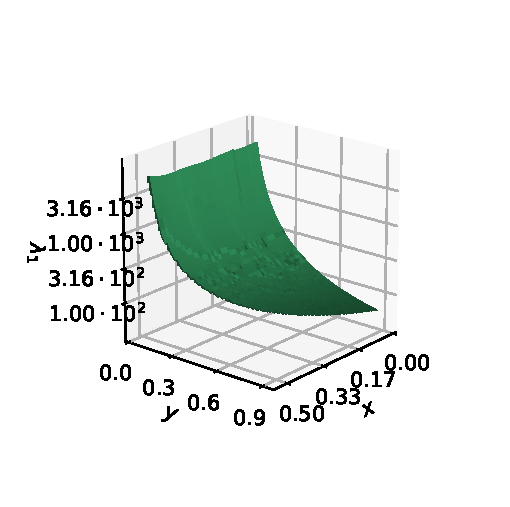
\includegraphics[width = 64.5mm]{figures/eigenvalues_3D.pdf}
        \caption{Prostorni pogled}
        \label{fig:triangles_eigenvalues_spatial}
    \end{subfigure}
    \begin{subfigure}{74mm}
        \centering
        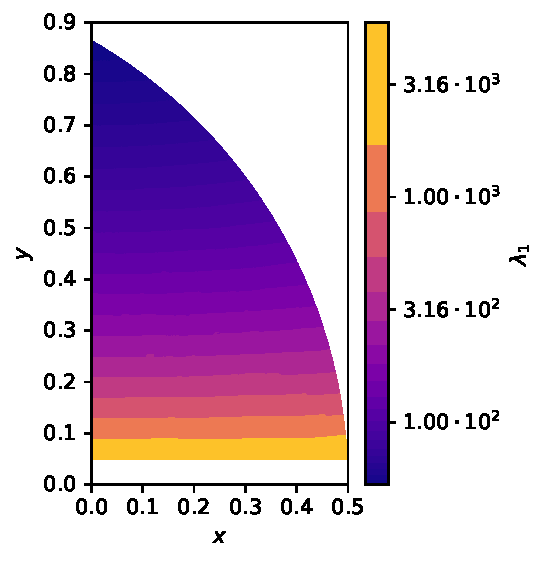
\includegraphics[width = 69mm]{figures/eigenvalues.pdf}
        \caption{Tlocrtni pogled}
        \label{fig:triangles_eigenvalues_contour}
    \end{subfigure}
    \caption[Najmanje svojstvene vrijednosti Laplaceovog operatora na trokutima]{Najmanje svojstvene vrijednosti Laplaceovog operatora na trokutima. Slike prikazuju funkciju koja točki \ensuremath{V \in D_{{\bigtriangleup}}}, gdje je \ensuremath{D_{{\bigtriangleup}}} skup iz propozicije~\ref{prop:triangle_characteristic_bijective}, pridružuje najmanju svojstvenu vrijednost Laplaceovog operatora na otvorenom trokutu čiji su vrhovi \ensuremath{\left( \frac{\numprint{1}}{\numprint{2}} , \numprint{0} \right) , V , \left( {- \frac{\numprint{1}}{\numprint{2}}} , \numprint{0} \right)}. Iz tehničkih razloga svojstvene vrijednosti na točkama \emph{ispod} pravca \ensuremath{y = \numprint{0.05}} nije bilo moguće izračunati, ali vrijednosti neograničeno rastu kada vrijednost ordinate teži u \ensuremath{\numprint{0}}. Najmanja prikazana vrijednost iznosi \ensuremath{\numprint{52.7248}}, a najveća \ensuremath{\numprint{5938.1931}} (vrijednosti su na dijagramima prikazane u logaritamskoj skali).}
    \label{fig:triangles_eigenvalues}
\end{figure}

\par%
\clearpage%
\newpage

Originalni skup trokuta nije pogodan za konstrukciju modela. Naime, kao što je vidljivo iz slike~\ref{fig:triangles_eigenvalues}, rast najmanje svojstvene vrijednosti vrlo je brz s obzirom na pad vrijednosti ordinate trećeg vrha trokuta pa je zbog ekvidistantnosti mreže neproporcionalno više točaka u skupu $ D_{{\bigtriangleup}} $ generirano s \emph{većom} najmanjom svojstvenom vrijednosti. Skup podataka stoga je potrebno prvo \emph{uravnotežiti}\footnote{Zapravo, legitimno je tvrditi da je realna situacija da su \emph{ekstremno velike} najmanje svojstvene vrijednosti puno zastupljenije nego \emph{manje} jer, kada bi se uniformno slučajno birala točka u skupu $ D_{{\bigtriangleup}} $ iz propozicije~\ref{prop:triangle_characteristic_bijective}, veća je vjerojatnost da će najmanja svojstvena vrijednost Laplaceovog operatora na dobivenom trokutu biti \emph{velika} nego da će biti \emph{mala}. Međutim, za konstrukciju modela strojnog učenja poželjno je da se on ne \emph{pretrenira} na velikim vrijednostima, nego da dobro predviđa i manje vrijednosti. Relativno mala greška na \emph{ekstremno velikim} vrijednostima velika je greška na \emph{malim} vrijednostima, stoga bi neuravnotežena zastupljenost \emph{ekstremno velikih} vrijednosti mogla katastrofalno utjecati na uspješnost modela na \emph{malim} vrijednostima.}.

\par

\begin{remark} \label{rem:point_Laplacian_eigenvalue}
    U daljnjem tekstu, kada će se spominjati najmanja svojstvena vrijednost Laplaceovog operatora u kontekstu s jedinstvenom točkom odnosno njezinom vrijednosti apscise i/ili ordinate (na primjer, ovisnost najmanje svojstvene vrijednosti Laplaceovog operatora o vrijednosti ordinate), tada će se, zapravo, govoriti o preslikavanju sa slike~\ref{fig:triangles_eigenvalues}.
\end{remark}

\par

\subsection{Uravnoteženje podataka}

\par

Na slici~\ref{fig:triangles_eigenvalues} vidljivo je da je najmanja svojstvena vrijednost relativno konstantna za konstantnu vrijednost ordinate (za razliku od varijabilnosti s obzirom na fiksiranu vrijednost apscise). Stoga je generiran pomoćni skup trokuta, takav da je interval $ \intervalcc{\numprint{0}}{\frac{\sqrt{\numprint{3}}}{\numprint{2}}} $ diskretiziran opet istim točkama kao u prvom slučaju, a za svaku vrijednost $ y_{j} $ te diskretizacije dužina dobivena presjekom skupa $ D_{{\bigtriangleup}} $ i pravca $ y = y_{j} $ ekvidistantno je podijeljena na $ \numprint{5} $ točaka. Točnije, generirane su vrijednosti na krivuljama
\begin{equation*}
    x = p \left( {- \frac{\numprint{1}}{\numprint{2}}} + \sqrt{\numprint{1} - y^{\numprint{2}}} \right) , \quad p \in \left\{ \numprint{0} , \frac{\numprint{1}}{\numprint{4}} , \frac{\numprint{1}}{\numprint{2}} , \frac{\numprint{3}}{\numprint{4}} , \numprint{1} \right\}
\end{equation*}
(tako da je $ \left( p^{{- \numprint{1}}} x + \frac{\numprint{1}}{\numprint{2}} \right)^{\numprint{2}} + y^{\numprint{2}} = \numprint{1} $ ako je $ p \neq \numprint{0} $; inače je, očito, $ x = \numprint{0} $) u skupu $ D_{{\bigtriangleup}} $, u onim vrijednostima $ y \in \intervaloc{\numprint{0}}{\frac{\sqrt{\numprint{3}}}{\numprint{2}}} $ iz originalne ekvidistantne mreže. U tim su točkama (trokutima) ponovo izračunate najmanje svojstvene vrijednosti.

\par

Za svaki generirani trokut (u originalnom skupu podataka i u pomoćnom) izračunate su duljine stranica, veličine vanjskih kutova, singularne vrijednosti duljina stranica, singularne vrijednosti vanjskih kutova i, naravno, najmanja svojstvena vrijednost Laplaceovog operatora. \emph{Spojimo} te vrijednosti u vektor (redak tablice) i označimo skup takvih zapisa o trokutima (tablicu) na prvotnom skupu s $ A $, a na pomoćnom skupu s $ B $. Elemente skupova $ A $ i $ B $ označavat ćemo s $ \asvector{t} $---svaki takav element vektor je informacija o trokutu---a \emph{zapis} o najmanjoj svojstvenoj vrijednosti u vektoru $ \asvector{t} $ označavat ćemo s $ \asvector{t}{\text{\texttt{[}} \lambda \text{\texttt{]}}} $. Označimo i multiskupove
\begin{align*}
    A{\text{\texttt{[}} \lambda \text{\texttt{]}}} & \coloneqq \left\{ \asvector{t}{\text{\texttt{[}} \lambda \text{\texttt{]}}} : \asvector{t} \in A \right\} \text{,} \\
    B{\text{\texttt{[}} \lambda \text{\texttt{]}}} & \coloneqq \left\{ \asvector{t}{\text{\texttt{[}} \lambda \text{\texttt{]}}} : \asvector{t} \in B \right\} \text{.}
\end{align*}

\par

Tada su izračunate vrijednosti kvantila dvadesetina $ \lambda_{\numprint{0.00}} \leq \lambda_{\numprint{0.05}} \leq \lambda_{\numprint{0.10}} \leq \dotsb \leq \lambda_{\numprint{1.00}} $ skupa $ B{\text{\texttt{[}} \lambda \text{\texttt{]}}} $ (zapravo je, dodatno, uzeto $ \lambda_{\numprint{0.00}} = \min \left( A{\text{\texttt{[}} \lambda \text{\texttt{]}}} \cup B{\text{\texttt{[}} \lambda \text{\texttt{]}}} \right) - \varepsilon $ i $ \lambda_{\numprint{1.00}} = \max \left( A{\text{\texttt{[}} \lambda \text{\texttt{]}}} \cup B{\text{\texttt{[}} \lambda \text{\texttt{]}}} \right) + \varepsilon $ za neki $ \varepsilon > \numprint{0} $). S ovim vrijednostima skup $ A $ je particioniran na skupove $ A_{\numprint{0.05}} , A_{\numprint{0.10}} , \dotsc , A_{\numprint{1.00}} \subseteq A $ definirane s
\begin{equation*}
    A_{p} \coloneqq \left\{ \asvector{t} \in A : \lambda_{p - \numprint{0.05}} \leq \asvector{t}{\text{\texttt{[}} \lambda \text{\texttt{]}}} < \lambda \right\} \subseteq A , \quad \forall p \in \left\{ \numprint{0.05} , \numprint{0.10} , \dotsc , \numprint{1.00} \right\} \text{,}
\end{equation*}
Dobiveni skup $ A_{\numprint{0.95}} $ bio je najveći, i to više od $ \numprint{15} $ puta veći nego $ A_{\numprint{0.05}} $, koji je bio najmanji. S druge strane, kako su granice definiranih skupova zapravo granice jednako velikih kvantila multiskupa $ B{\text{\texttt{[}} \lambda \text{\texttt{]}}} $, tako definirani dijelovi skupa $ B $ bili bi podjednako veliki. Dijelovi skupa $ D_{{\bigtriangleup}} $ na slici~\ref{fig:triangles_eigenvalues_contour} zapravo su obojani s obzirom na najmanju svojstvenu vrijednost Laplaceovog operatora u $ \numprint{20} $ nijansi od kojih svaka pripada jednom od kvantilnih intervala $ \intervalco{\lambda_{p - \numprint{0.05}}}{\lambda_{p}} $.

\par

Konačno je, za zadani $ n \in \positives{\naturals} $, iz svakog od skupova $ A_{\numprint{0.05}} , A_{\numprint{0.10}} , \dotsc , A_{\numprint{1.00}} $ slučajnim odabirom uzeto po $ n $ različitih zapisa, čime je konstruiran treći, novi skup $ A ' \subseteq A $. Pritom se zahtijevalo da varijanca svake kategorije podataka u izabranom podskupu $ A_{p} ' $ skupa $ A_{p} \in \left\{ A_{\numprint{0.05}} , A_{\numprint{0.10}} , \dotsc , A_{\numprint{1.00}} \right\} $ ostane što sličnija varijanci te kategorije podataka u skupu $ A_{p} $.

\par

Na slici~\ref{fig:dataset_balanced_discretisation} prikazan je rezultat opisanog postupka za $ n = \numprint{50} $ (ukupno $ \numprint{1000} $ točaka, u odnosu na originalnih $ \numprint{1129741} $).

\par

\begin{figure}[htb!]
    \centering
    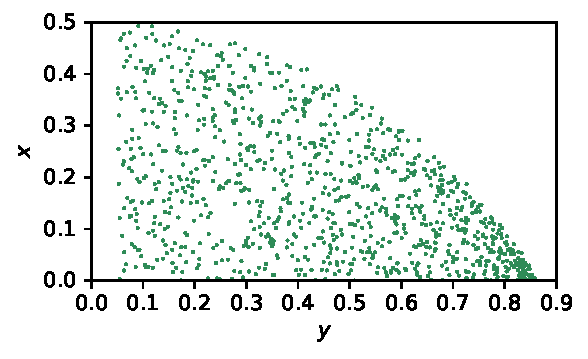
\includegraphics[width = 80mm]{figures/sample.pdf}
    \caption{\emph{Uravnotežena} diskretizacija skupa \ensuremath{D_{{\bigtriangleup}}} iz propozicije~\ref{prop:triangle_characteristic_bijective}}
    \label{fig:dataset_balanced_discretisation}
\end{figure}

\par

\section{Izrada skupa podataka za treniranje, validaciju i testiranje}
\label{sec:dataset_split}

Osnovna ideja bila je predodrediti $ {{\sim} \unit[\numprint{70}]{\%}} $ podataka za treniranje, $ {{\sim} \unit[\numprint{15}]{\%}} $ podataka za validaciju i $ {{\sim} \unit[\numprint{15}]{\%}} $ podataka za testiranje. Kod modela kod kojih validacija nije potrebna---zapravo, samo kod linearne regresije---podatci za validaciju spojeni su s podatcima za testiranje u veći skup podataka za testiranje, koji čini $ {{\sim} \unit[\numprint{30}]{\%}} $ svih podataka.

\par

\subsection{Izrada skupa podataka za treniranje, validaciju i testiranje za modele s isključivo numeričkim ulaznim podatcima}

\par

Kako sva korištena numerička obilježja trokuta (poligona) ne ovise o položaju, orijentaciji i rotaciji trokuta u ravnini, kod izrade skupova podataka za modele koji primaju isključivo numeričke podatke nije bilo potrebno generirati više reprezentanata sličnih trokuta (zapravo, sukladnih jer su svi trokuti istog dijametra). Stoga je za takve modele bilo moguće s istim brojem podataka obuhvatiti veći broj slučajeva.

\par

Opisanom metodom za uravnoteženje podataka ukupni skup podataka za ove modele dobiven je tako da se iz skupa $ A_{p} $ biralo $ \min \left( \left\{ \card \left( A_{\numprint{0.00}} \right) , \card \left( A_{\numprint{0.05}} \right) , \dotsc , \card \left( A_{\numprint{1.00}} \right) \right\} \right) $ podataka, za svaki $ p \in \left\{ \numprint{0.00} , \numprint{0.05} , \dotsc , \numprint{1.00} \right\} $. Tada je na dobivenom skupu $ A ' $ ponovljen postupak tako da se dobije skup $ A '' $ čiji je kardinalitet otprilike $ \unit[\numprint{30}]{\%} $ kardinaliteta skupa $ A ' $, ali ovdje se što vjernija varijanca (što sličnija varijanci na $ A_{p} ' $, a ne prvotnoj na $ A_{p} $) pokušala zadržati ne samo na $ A_{p} '' $, nego i na $ A_{p} ' \setminus A_{p} '' $. Na kraju se na skupu $ A '' $ isti postupak ponovio generirajući skup $ A ''' $ kardinaliteta upola manjeg nego $ A '' $, pri čemu se i ovdje originalna varijanca (varijanca iz skupa $ A_{p} '' $, a ne iz $ A_{p} ' $ ili $ A_{p} $) zadržavala na biranim dijelovima i na njihovim komplementima. Tako dobiveni skupovi su
\begin{enumerate}
    \item skup podataka za treniranje: $ A ' \setminus A '' $---ukupno $ \numprint{76280} $ trokuta,
    \item skup podataka za validaciju: $ A '' \setminus A ''' $---ukupno $ \numprint{16340} $ trokuta,
    \item skup podataka za testiranje: $ A ''' $---ukupno $ \numprint{16340} $ trokuta.
\end{enumerate}

\par

\subsection{Izrada skupa podataka za treniranje, validaciju i testiranje za modele s vizualnim ulaznim podatcima}

Budući da vizualna karakterizacija poligona ovisi o njegovu položaju, rotaciji i orijentaciji, za generiranje reprezentativnog skupa podataka s vizualnim karakterizacijama bilo je potrebno uključiti pojedine perturbacije trokuta. Tako je originalni skup podataka prvo povećan dodavanjem refleksija oko ordinate svih trokuta (uključujući i jednakokračnih i jednakostraničnog, iako su oni simetrični), a zatim rotiranjem svakog trokuta $ \numprint{10} $ puta za pseudoslučajno izabrani kut. Trokuti su bili rotirani neovisno jedan o drugme, štoviše, svaka od $ \numprint{10} $ rotacija svakog trokuta bila je neovisna o drugim rotacijama. Kut rotacije birao se uniformno pseudoslučajno iz skupa $ \intervalco{\numprint{0}}{\numprint{2} \pi} $. Konačno je opisanim postupkom dobiveno $ \numprint{22594820} $ trokuta. Ovi su trokuti zatim translatirani tako da im središte upisane kružnice bude u ishodištu (u točki $ \left( 0 , 0 \right) $).

\par

Dobiveni je skup tada bio reduciran do uravnoteženog skupa $ A ' $ od \emph{svega} $ \numprint{100000} $ trokuta (zbog ograničenih resursa varijanca se računala samo na singularnim vrijednostima duljina stranica i vanjskih kutova i na najmanjim svojstvenim vrijednostima Laplaceovog operatora). Zatim su, analognim postupkom kao kod generiranja skupa podataka za modele s isključivo numeričkim ulaznim podatcima, ekstrahirani skupovi za validaciju $ A '' \setminus A ''' $ i testiranje $ A ''' $ (ovdje su se uzimale u obzir varijance svih obilježja i ciljne varijable). Konačni kardinaliteti skupova iznosili su
\begin{enumerate}
    \item skup podataka za treniranje: $ A ' \setminus A '' $---ukupno $ \numprint{70000} $ trokuta,
    \item skup podataka za validaciju: $ A '' \setminus A ''' $---ukupno $ \numprint{15000} $ trokuta,
    \item skup podataka za testiranje: $ A ''' $---ukupno $ \numprint{15000} $ trokuta.
\end{enumerate}

\par

\section{Eksploratorna analiza numeričkih podataka}
\label{sec:dataset_exploratory_analysis}

U eksploratornoj analizi podataka postupkom uravnotežavanja podataka iz numeričkog skupa podataka za treniranje ekstrahirano je $ \numprint{1000} $ točaka (po $ \numprint{50} $ iz svakog dijela) za vizualizaciju komentiranih zavisnosti radi bolje preglednosti. Kako su dijagrami bili gotovo isti pri svakom novom generiranju takvog podskupa, rezultati koji su predstavljeni vizualno su reprezentativni. Ipak, osim vizualizacije predstavljene su i numeričke vrijednosti koje su izračunate na cijelom skupu podataka za treniranje.

\par

Iako stvarna najmanja svojstvena vrijednost ima \emph{jako} konveksan oblik i brz rast s obzirom na pad ordinate (\seetxt~sliku~\ref{fig:triangles_eigenvalues}), njezin multiplikativni inverz gotovo pa je linearan s obzirom na vrijednost ordinate---Pearsonov koeficijent korelacije iznosi čak $ \unit[\numprint{99.8239}]{\%} $, što je najveći opaženi koeficijent korelacije (po apsolutnoj vrijednosti). S druge strane, za \emph{relativno fiksnu} vrijednost ordinate (zadanu da bude u nekom \emph{užem} intervalu), multiplikativni inverz najmanje svojstvene vrijednosti opada u blagom luku s porastom vrijednosti apscise. Ove su ovisnosti prikazane na slici~\ref{fig:x_y_eigenvalue}.

\par%
\clearpage%
\newpage

\begin{figure}[htb!]
    \centering
    \begin{subfigure}{51.4mm}
        \centering
        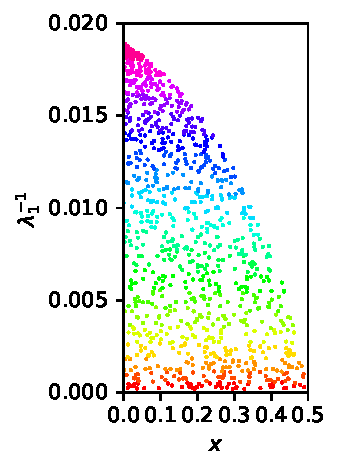
\includegraphics[width = 46.4mm]{figures/x-lambda.pdf}
        \caption{Apscisa}
        \label{fig:x_y_eigenvalues_abscissa}
    \end{subfigure}
    \begin{subfigure}{76.2mm}
        \centering
        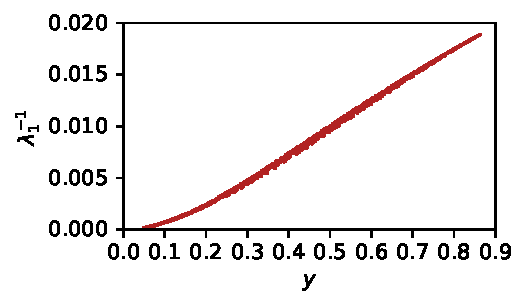
\includegraphics[width = 71.2mm]{figures/y-lambda.pdf}
        \caption{Ordinata}
        \label{fig:x_y_eigenvalues_ordinate}
    \end{subfigure}
    \caption[Ovisnosti multiplikativnog inverza najmanje svojstvene vrijednosti Laplaceovog operatora na trokutima dijametra \ensuremath{\numprint{1}} u odnosu na koordinate karakterističnih točaka iz propozicije~\ref{prop:triangle_characteristic_bijective}]{Ovisnosti multiplikativnog inverza najmanje svojstvene vrijednosti Laplaceovog operatora na trokutima dijametra \ensuremath{\numprint{1}} u odnosu na koordinate karakterističnih točaka iz propozicije~\ref{prop:triangle_characteristic_bijective}. Na slici~\ref{fig:x_y_eigenvalues_abscissa} točke su obojane s obzirom na vrijednosti ordinate po kvantilima zastupljenosti u skupu podataka za treniranje.}
    \label{fig:x_y_eigenvalue}
\end{figure}

\par

Kao što je vidljivo na slici~\ref{fig:triangles_eigenvalues}, na bilo kojoj kružnici sa središtem u točki $ \left( {- \frac{\numprint{1}}{\numprint{2}} } , \numprint{0} \right) $, koja sa skupom $ D_{{\bigtriangleup}} $ ima zajedničkih točaka, svojstvene vrijednosti pojavljuju se u nekom samo slijeva ograničenom intervalu. Radijus takvih kružnica zapravo je duljina druge najdulje stranice trokuta koje te točke u skupu $ D_{{\bigtriangleup}} $ predstavljaju, stoga je jasno da najmanja svojstvena vrijednost Laplaceovog operatora nema izraženu korelaciju s drugom najduljom stranicom trokuta. Isto tako, svim trokutima najdulja je stranica duljine $ \numprint{1} $ pa korelacija najmanje svojstvene vrijednosti i duljine najdulje stranice (za trokute fisknog dijametra) uopće ne postoji. Tek je postojeća korelacija s duljinom najkraće stranice, kao što je vidljivo na slici~\ref{fig:edge_angle_eigenvalue}, a čiji Pearsonov koeficijent korelacije iznosi $ \unit[\numprint{94.8912}]{\%} $. Na toj su slici prikazane i ovisnosti o vanjskim kutovima, od čijih korelacija valja spomenuti korelaciju s najvećim vanjskim kutom (suplementom najmanjeg unutarnjeg kuta), čiji Pearsonov koeficijent korelacije iznosi $ {- \unit[\numprint{97.8601}]{\%}} $.

\par%
\clearpage%
\newpage

\begin{figure}[htb!]
    \centering
    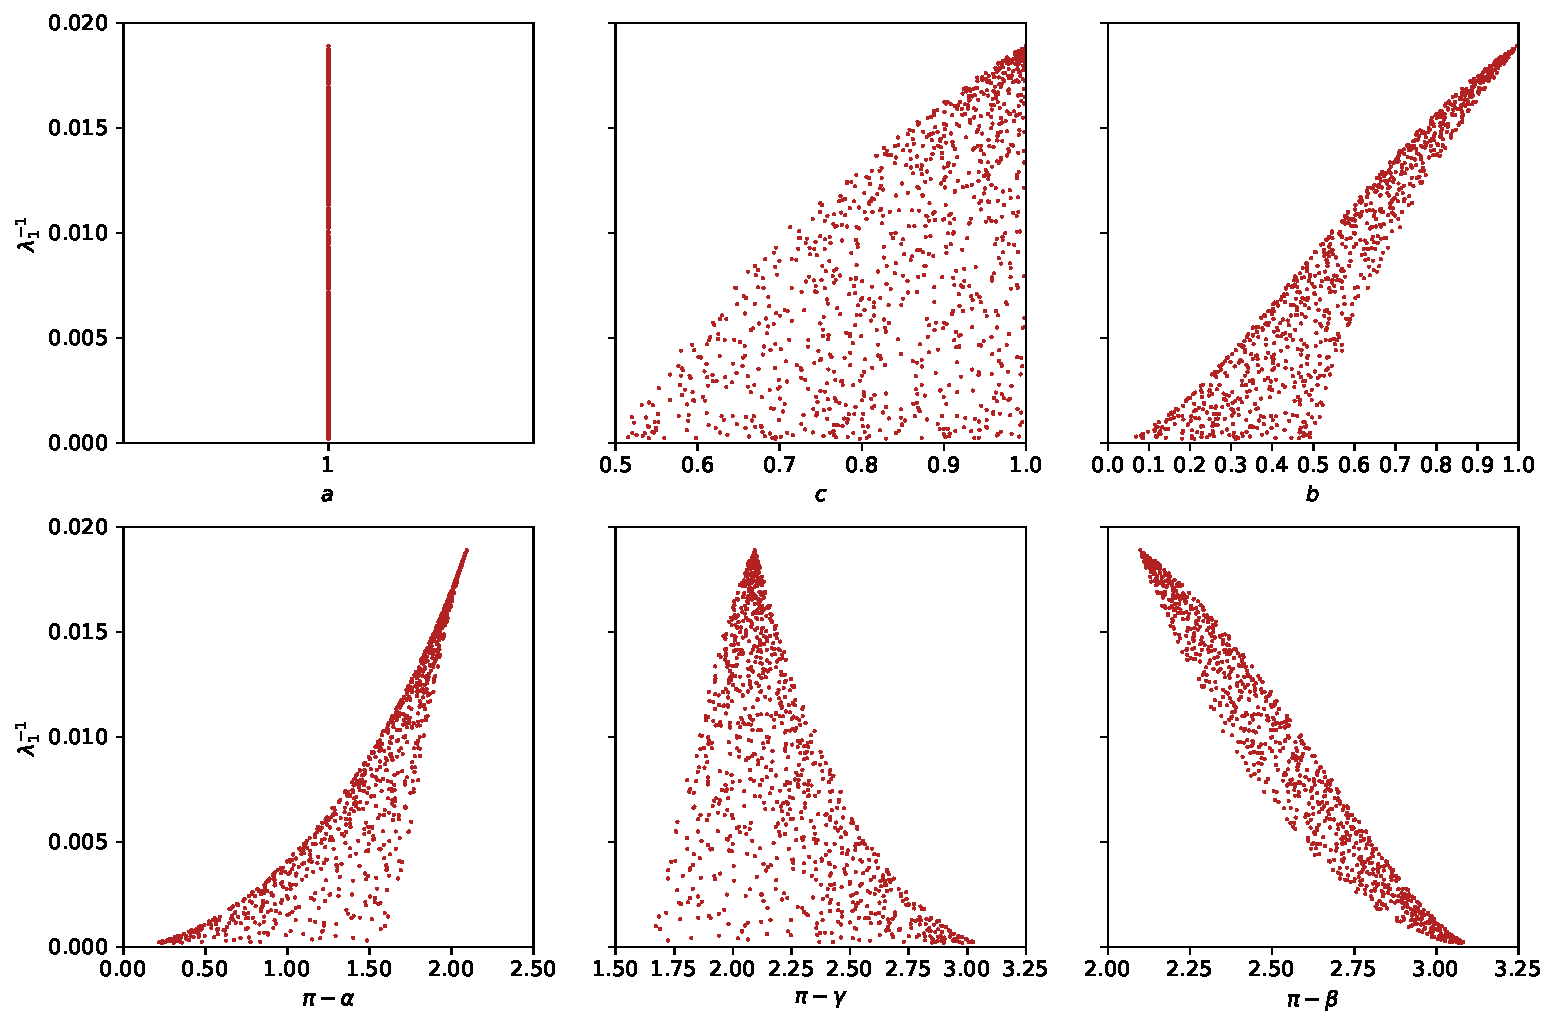
\includegraphics[width = 132mm]{figures/edge_angle-lambda.pdf}
    \caption[Ovisnosti multiplikativnog inverza najmanje svojstvene vrijednosti Laplaceovog operatora na trokutima dijametra \ensuremath{\numprint{1}} u odnosu na duljine stranica i veličine vanjskih kutova]{Ovisnosti multiplikativnog inverza najmanje svojstvene vrijednosti Laplaceovog operatora na trokutima dijametra \ensuremath{\numprint{1}} u odnosu na duljine stranica i veličine vanjskih kutova. Duljine stranica trokuta označene su tako da je \ensuremath{a \geq c \geq b}, a unutarnji kutovi tako da je \ensuremath{\alpha \geq \gamma \geq \beta} (vanjski kutovi su tada \ensuremath{\pi - \alpha \leq \pi - \gamma \leq \pi - \beta}).}
    \label{fig:edge_angle_eigenvalue}
\end{figure}

\par

Slično kao što je korelacija najmanje svojstvene vrijednosti s duljinom najdulje stranice nepostojeća zbog fiksne duljine najdulje stranice, uzimajući u obzir slutnju~\ref{conj:polygon_characteristic_angle_fixed} za očekivati je i da je nepostojeća korelacija s najvećom singularnom vrijednosti vanjskih kutova. Međutim, ovdje je ta korelacija nepostojeća čak i ako dijametar trokuta nije fiksan jer vanjski kutovi ne ovise o dijametru poligona. Također, zbog slutnje~\ref{conj:polygon_characteristic_number_of_values} za očekivati je da je dovoljno proučavati samo dvije najveće singularne vrijednosti duljina stranica i vanjskih kutova, a ne sve tri (ako uopće ima smisla proučavati najveću singularnu vrijednosti vanjskih kutova). Ovisnosti najmanje svojstvene vrijednosti o ovim singularnim vrijednostima prikazane su na slici~\ref{fig:singular_value_eigenvalue}.

\par

Osim najveće singularne vrijednosti vanjskih kutova, sve ostale singularne vrijednosti s multiplikativnim inverzom najmanje svojstvene vrijednosti Laplaceovog operatora imaju Pearsonov koeficijent korelacije po apsolutnoj vrijednosti veći od $ \unit[\numprint{90}]{\%} $. Koeficijenti iznose: $ \unit[\numprint{99.1195}]{\%} $ za najveću singularnu vrijednost duljina stranica---što je najveća korelacija (po apsolutnoj vrijednosti) izuzev korelacije vrijednosti ordinate i korelacija kasnije spomenutih složenih značajki---$ {- \unit[\numprint{93.3544}]{\%}} $ za drugu i treću najveću singularnu vrijednost duljina stranica i $ {- \unit[\numprint{94.6484}]{\%}} $ za drugu i treću najveću singularnu vrijednost vanjskih kutova.

\par

\begin{figure}[htb!]
    \centering
    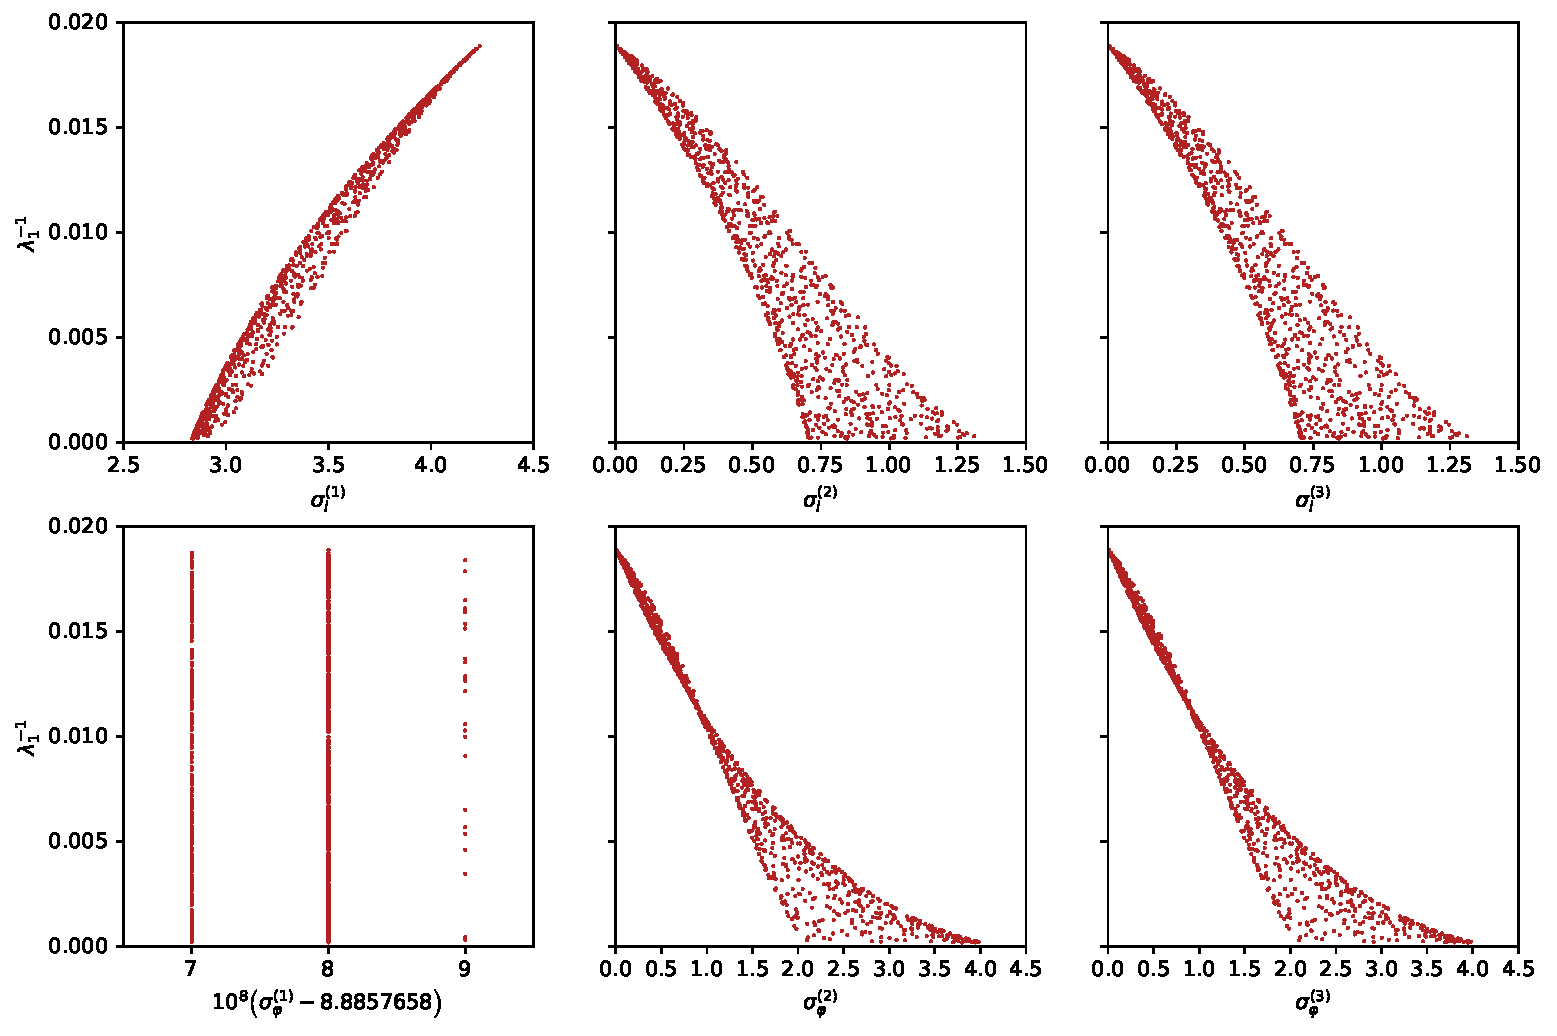
\includegraphics[width = 132mm]{figures/sv-lambda.pdf}
    \caption[Ovisnosti multiplikativnog inverza najmanje svojstvene vrijednosti Laplaceovog operatora na trokutima dijametra \ensuremath{\numprint{1}} u odnosu na singularne vrijednosti duljina stranica i vanjskih kutova]{Ovisnosti multiplikativnog inverza najmanje svojstvene vrijednosti Laplaceovog operatora na trokutima dijametra \ensuremath{\numprint{1}} u odnosu na singularne vrijednosti duljina stranica i vanjskih kutova. Vektor \ensuremath{\sigma_{l} = \left( \sigma_{l}^{\left( \numprint{1} \right)} , \sigma_{l}^{\left( \numprint{2} \right)} , \sigma_{l}^{\left( \numprint{3} \right)} \right) \in \intervalco{\numprint{0}}{{+ \infty}}^{\numprint{3}}} vektor je singularnih vrijednosti duljina stranica, a vektor \ensuremath{\sigma_{\varphi} = \left( \sigma_{\varphi}^{\left( \numprint{1} \right)} , \sigma_{\varphi}^{\left( \numprint{2} \right)} , \sigma_{\varphi}^{\left( \numprint{3} \right)} \right) \in \intervalco{\numprint{0}}{{+ \infty}}^{\numprint{3}}} vektor je singularnih vrijednosti vanjskih kutova (uređeni su silazno tako da se svaka singularna vrijednost pojavljuje onoliko puta kolika joj je kratnost).}
    \label{fig:singular_value_eigenvalue}
\end{figure}

\par

Slika~\ref{fig:singular_value_eigenvalue} i izračunati koeficijenti korelacije daju naslutiti da je vrlo čvrsta korelacija najmanje svojstvene vrijednosti s najvećom singularnom vrijednosti duljina stranica. Varijabilnost najveće singularne vrijednosti vanjskih kutova, koja je \emph{širine} $ \numprint{2} \cdot \numprint{10}^{{- \numprint{8}}} $, vidljiva na toj slici lako je moguće rezultat greške numeričkog računa, a ne da ona stvarno varira (\seetxt~slutnju~\ref{conj:polygon_characteristic_angle_fixed}).

\par

Na slici~\ref{fig:singular_value_eigenvalue} dodatno se vidi da druga i treća singularna vrijednost duljina stranica odnosno vanjskih kutova ima istu korelaciju s najmanjom svojstvenom vrijednosti Laplaceovog operatora. Ova pojava još je jasnija kada proučimo korelaciju druge i treće singularne vrijednosti, koja je prikazana na slici~\ref{fig:2_3_singular_value}---te su singularne vrijednosti zapravo jednake. Ovaj je fenomen već bio najavljen slutnjom~\ref{conj:polygon_characteristic_number_of_values}.

\par%
\clearpage%
\newpage

\begin{figure}[htb!]
    \centering
    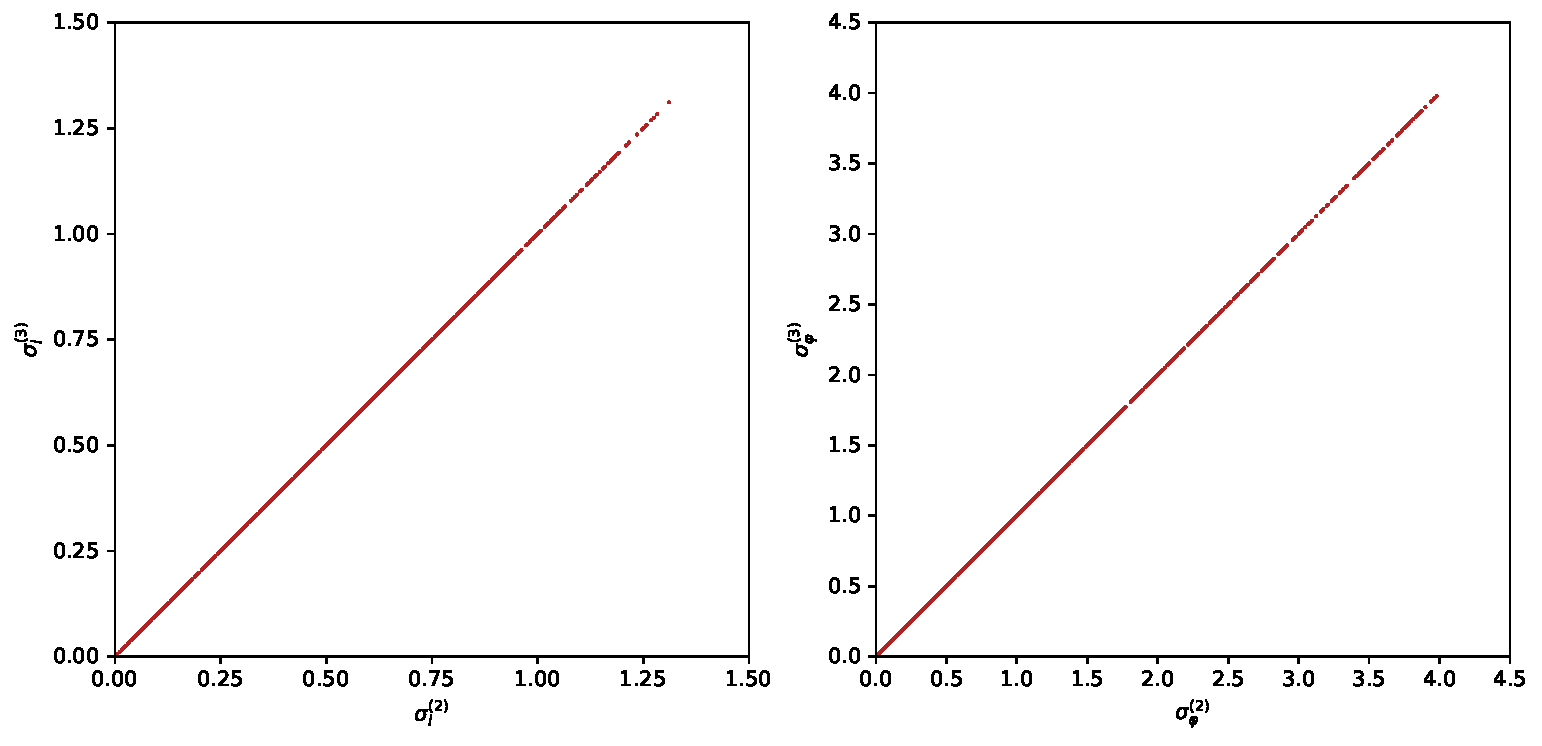
\includegraphics[width = 129.5mm]{figures/sv-sv.pdf}
    \caption[Ovisnosti druge i treće singularne vrijednosti duljina stranica odnosno vanjskih kutova na trokutima dijametra \ensuremath{\numprint{1}}]{Ovisnosti druge i treće singularne vrijednosti duljina stranica odnosno vanjskih kutova na trokutima dijametra \ensuremath{\numprint{1}}. Vektor \ensuremath{\sigma_{l} = \left( \sigma_{l}^{\left( \numprint{1} \right)} , \sigma_{l}^{\left( \numprint{2} \right)} , \sigma_{l}^{\left( \numprint{3} \right)} \right) \in \intervalco{\numprint{0}}{{+ \infty}}^{\numprint{3}}} vektor je singularnih vrijednosti duljina stranica, a vektor \ensuremath{\sigma_{\varphi} = \left( \sigma_{\varphi}^{\left( \numprint{1} \right)} , \sigma_{\varphi}^{\left( \numprint{2} \right)} , \sigma_{\varphi}^{\left( \numprint{3} \right)} \right) \in \intervalco{\numprint{0}}{{+ \infty}}^{\numprint{3}}} vektor je singularnih vrijednosti vanjskih kutova (uređeni su silazno tako da se svaka singularna vrijednost pojavljuje onoliko puta kolika joj je kratnost).}
    \label{fig:2_3_singular_value}
\end{figure}

\par

Osim spomenutih korelacija, proučavane su i \emph{složenije} korelacije tako da se od dvije značajke izračuna nova, treća značajka i onda proučava njezina korelacija s najmanjom svojstvenom vrijednosti. Od takvih proučavanih korelacija najbolje rezultate imale su značajke definirane s
\begin{align*}
    f_{\numprint{1}} \left( a , b \right) & \coloneqq \sqrt{\left( \frac{a}{A} \right)^{\numprint{2}} + \left( \frac{b}{B} \right)^{\numprint{2}}} \text{,} \\
    f_{\numprint{2}} \left( a , b \right) & \coloneqq \sqrt{\left( \frac{a}{A} \right)^{\numprint{2}} + \left( \frac{B - b}{B} \right)^{\numprint{2}}} \text{,} \\
    f_{\numprint{3}} \left( a , b \right) & \coloneqq \sqrt{\left( \frac{A - a}{A} \right)^{\numprint{2}} + \left( \frac{b}{B} \right)^{\numprint{2}}} \text{,} \\
    f_{\numprint{4}} \left( a , b \right) & \coloneqq \sqrt{\left( \frac{A - a}{A} \right)^{\numprint{2}} + \left( \frac{B - b}{B} \right)^{\numprint{2}}} \text{,}
\end{align*}
gdje su $ a , b $ vrijednosti nekih originalnih značajki (na primjer, drugi najveći vanjski kut ili najveća singularna vrijednost duljina stranica), a $ A , B $ najveće opažene vrijednosti tih značajki u skupu podataka za treniranje (mogu biti teorijski izračunate vrijednosti ako je poznat maksimum ili supremum promatrane značajke, kao, na primjer, $ \pi $ za najveći vanjski kut). Definirane značajke možemo shvatiti kao euklidske norme točaka u ravnini čije su koordinate dane izrazima $ \frac{a}{A} $ ili $ \frac{A - a}{A} $ i $ \frac{b}{B} $ ili $ \frac{B - b}{B} $. Značajke su u tim izrazima normirane zato što različite značajke imaju različite raspone vrijednosti pa kvadriranjem veća od tih značajki još jače dominira u izrazu $ a^{\numprint{2}} + b^{\numprint{2}} $. Ovisnosti najmanje svojstvene vrijednosti Laplaceovog operatora o dvama ovakvim značajkama dobivenim od druge najveće singularne vrijednosti duljina stranica i druge najveće singularne vrijednosti vanjskih kutova prikazane su na slici~\ref{fig:norm_singular_value_singular_value_eigenvalue}.

\par

\begin{figure}[htb!]
    \centering
    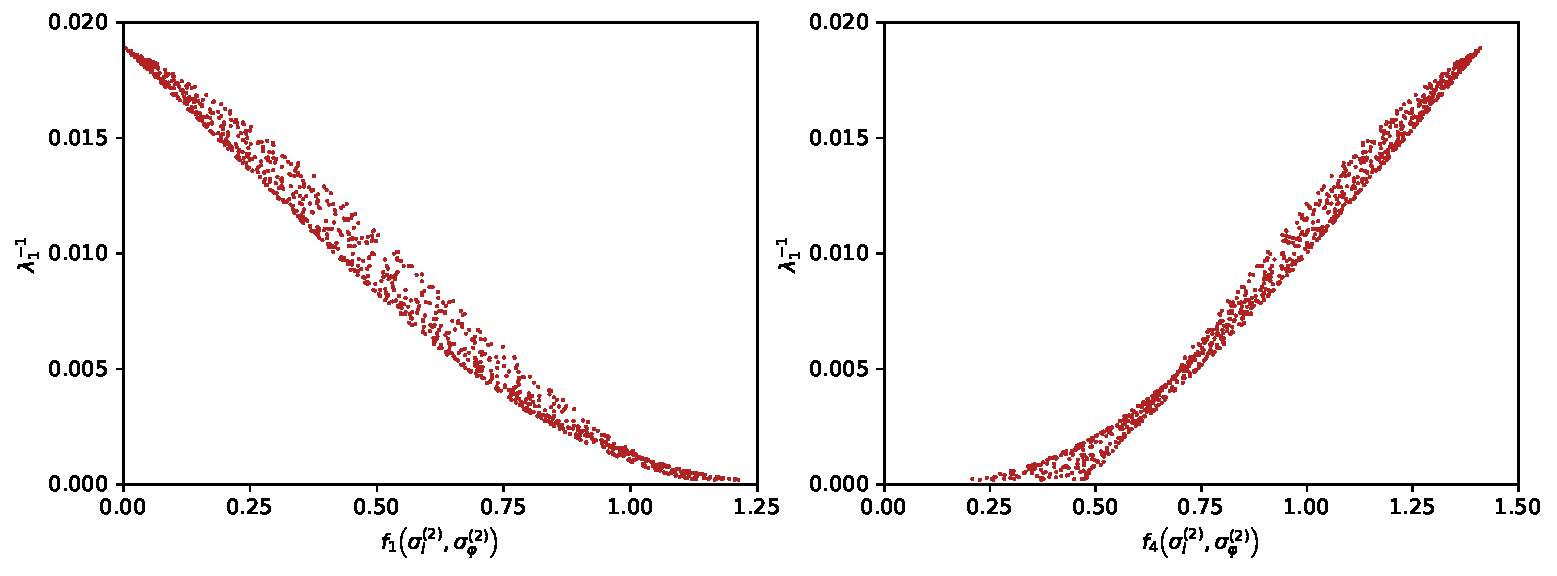
\includegraphics[width = 132mm]{figures/r(sv,sv)-lambda.pdf}
    \caption[Ovisnosti multiplikativnog inverza najmanje svojstvene vrijednosti Laplaceovog operatora na trokutima dijametra \ensuremath{\numprint{1}} u odnosu na dodatne složene značajke]{Ovisnosti multiplikativnog inverza najmanje svojstvene vrijednosti Laplaceovog operatora na trokutima dijametra \ensuremath{\numprint{1}} u odnosu na dodatne složene značajke \ensuremath{f_{\numprint{1}}} i \ensuremath{f_{\numprint{4}}} dobivene od druge najveće singularne vrijednosti duljina stranica i druge najveće singularne vrijednosti vanjskih kutova. Vektor \ensuremath{\sigma_{l} = \left( \sigma_{l}^{\left( \numprint{1} \right)} , \sigma_{l}^{\left( \numprint{2} \right)} , \sigma_{l}^{\left( \numprint{3} \right)} \right) \in \intervalco{\numprint{0}}{{+ \infty}}^{\numprint{3}}} vektor je singularnih vrijednosti duljina stranica, a vektor \ensuremath{\sigma_{\varphi} = \left( \sigma_{\varphi}^{\left( \numprint{1} \right)} , \sigma_{\varphi}^{\left( \numprint{2} \right)} , \sigma_{\varphi}^{\left( \numprint{3} \right)} \right) \in \intervalco{\numprint{0}}{{+ \infty}}^{\numprint{3}}} vektor je singularnih vrijednosti vanjskih kutova (uređeni su silazno tako da se svaka singularna vrijednost pojavljuje onoliko puta kolika joj je kratnost).}
    \label{fig:norm_singular_value_singular_value_eigenvalue}
\end{figure}

\par

Od složenih značajki (ali proučavale su se samo one dobivene od duljina stranica, vanjskih kutova i singularnih vrijednosti, a bez koordinata točke u skupu $ D_{{\bigtriangleup}} $) čak $ \numprint{55} $ ih je imalo Pearsonov koeficijent korelacije s najmanjom svojstvenom vrijednosti Laplaceovog operatora po apsolutnoj vrijednosti veći od $ \unit[\numprint{90}]{\%} $, ali među njima su uglavnom dominirale iste originalne značajke koje i samostalno imaju apsolutno visoke koeficijente korelacije. Apsolutno veći od $ \unit[\numprint{95}]{\%} $ koeficijent korelacije imale su $ \numprint{34} $ značajke, apsolutno veći od $ \unit[\numprint{99}]{\%} $ njih $ \numprint{6} $, a najveći (po apsolutnoj vrijednosti) je koeficijent korelacije značajke $ f_{\numprint{3}} $ od najvećeg vanjskog kuta i najveće singularne vrijednosti duljina stranica, koji iznosi $ \unit[\numprint{99.4679}]{\%} $.

\par

Međutim, takve i složenije značajke u konačnom su se rješenju izbjegavale zato da dobiveni modeli budu što interpretativniji, generalizabilniji i neartificijelniji. Za rješavanje drugačijeg problema, ali također diferencijalne jednadžbe, Mills i dr.\ u~\cite{bib:Mills17} uopće nisu koristili vlastite izabrane numeričke značajke, nego su konstruirali uspješni model koji sam pronalazi značajke iz vizualnog prikaza dvodimenzionalnih elektrostatskih potencijala.

\par


    % Pregled razvijenih modela.
    \chapter{Razvijeni modeli}
\label{chp:models}

U sklopu ovog rada razvijeno je nekoliko modela strojnog učenja za predviđanju najmanje svojstvene vrijednosti Laplaceovog operatora na trokutima dijametra $ \numprint{1} $. Te modele možemo svrstati u tri skupine: linearna regresija, neuronske mreže i konvolucijske neuronske mreže. U ovom poglavlju objašnjene su arhitekture eksperimentalno pronađenih najboljih modela u svakoj skupini, a sami rezultati bit će predstavljeni tek u sljedećem poglavlju (u poglavlju~\ref{chp:results}).

\par

Osim pretprocesiranja \emph{golih} koordinata vrhova---u što ulaze računanje duljina stranica, veličina vanjskih kutova i singularnih vrijednosti duljina stranica i vanjskih kutova, koje je bilo realizirano u programskom jeziku \href{https://en.cppreference.com/w/c/header}{\emph{C}} sa standardnom bibliotekom, a za \emph{SVD} korištene su i biblioteke \href{http://www.netlib.org/blas/}{\emph{BLAS}} i \href{http://www.netlib.org/lapack/}{\emph{LAPACK}}---modeli su razvijani u programskom jeziku \href{https://docs.python.org/3/}{\emph{Python}} inačice $ \numprint{3} $ uz biblioteke \href{https://www.scipy.org/docs.html}{\emph{SciPy}} paketa (\href{https://numpy.org/}{\emph{NumPy}} i \href{https://pandas.pydata.org/}{\emph{Pandas}}). Kao platforma korištena je besplatna usluga \href{https://colab.research.google.com/}{\emph{Google Colab}} s ubrzanjem preko \emph{GPU}.

\par

\section{Linearna regresija}
\label{sec:linear_regression}

Jedna od ideja kod razvijanja modela bila je pronaći što jednostavniji model koji bi mogao dobro predviđati traženu vrijednost. Zbog neprekidnosti spektra iz teorema~\ref{thm:Laplace_eigenvalue_continuity} i karakterizacije trokuta pomoću jedinstvene točke u ograničenom povezanom skupu u ravnini iz propozicije~\ref{prop:triangle_characteristic_bijective} problem pronalaska najmanje svojstvene vrijednosti možemo pokušati aproksimirati polinomom u dvije varijable (koordinate karakteristične točke iz propozicije~\ref{prop:triangle_characteristic_bijective}).

\par

Polinom najviše $ n $-tog stupnja (ne navodimo ograničenje da je barem jedan od koeficijenata $ a_{\numprint{0} , n} , a_{\numprint{1} , n - \numprint{1}} , \dotsc , a_{n , \numprint{0}} $ različit od $ \numprint{0} $), za $ n \in \naturals $, linearna je kombinacija
\begin{multline*}
    P \left( x , y \right) = a_{\numprint{0} , \numprint{0}} + a_{\numprint{0} , \numprint{1}} y + a_{\numprint{1} , \numprint{0}} x + a_{\numprint{0} , \numprint{2}} y^{\numprint{2}} + a_{\numprint{1} , \numprint{1}} x y + a_{\numprint{2} , \numprint{0}} x^{\numprint{2}} + \dotsb + {} \\
    {} + a_{\numprint{0} , n} y^{n} + a_{\numprint{1} , n - \numprint{1}} x y^{n - \numprint{1}} + \dotsb + a_{n - \numprint{1} , \numprint{1}} x^{n - \numprint{1}} y + a_{n , \numprint{0}} x^{n} \text{,}
\end{multline*}
to jest, u kompaktnijem obliku
\begin{equation*}
    P \left( x , y \right) = \sum_{k = \numprint{0}}^{n} \sum_{i = \numprint{0}}^{k} a_{i , k - i} x^{i} y^{k - i}
\end{equation*}
(gdje, jednostavnosti zapisa radi, uzimamo $ \numprint{0}^{\numprint{0}} = \numprint{1} $ u slučaju da je $ x = \numprint{0} $ i/ili $ y = \numprint{0} $) za neke koeficijente $ a_{i j} $. Za poznati uzorak $ \left( \left( x_{i} , y_{i} , z_{i} \right) \right)_{i = \numprint{1}}^{N} $, gdje je $ N \in \naturals $ dovoljno velik, pronalazak polinoma stupnja najviše $ n $ koji najbolje aproksimira $ P \left( x , y \right) = z $ svodi se na linearnu regresiju.

\par

Najbolje rezultate s obzirom na kompleksnost modela lučili su polinomi stupnjeva $ \numprint{4} $ i $ \numprint{5} $ koji su predviđali multiplikativni inverz najmanje svojstvene vrijednosti Laplaceovog operatora. To jest, ako za proizvoljni otvoreni trokut dijametra $ \numprint{1} $ označimo s $ V = \left( x , y \right) \in \reals^{\numprint{2}} $ njegovu karakterističnu točku iz propozicije~\ref{prop:triangle_characteristic_bijective}, a s $ \lambda_{\numprint{1}} \in \intervaloo{\numprint{0}}{{+ \infty}} $ najmanju svojstvenu vrijednost Laplaceovog operatora na tom trokutu, onda su najbolji dobiveni polinomni modeli linearne regresije
\begin{equation*}
    \lambda_{\numprint{1}}^{{- \numprint{1}}} \approx \sum_{k = \numprint{0}}^{n} \sum_{i = \numprint{0}}^{k} a_{i , k - i}^{\left( n \right)} x^{i} y^{k - i} \text{,}
\end{equation*}
gdje je $ n \in \left\{ \numprint{4} , \numprint{5} \right\} $, a $ a_{i j}^{\left( n \right)} $ koeficijenti dobiveni linearnom regresijom za odgovarajući polinom.

\par

Nešto je bolje rezultate lučio model polinoma stupnja $ \numprint{11} $ koji je također predviđao multiplikativni inverz najmanje svojstvene vrijednosti, ali ta je razlika zanemariva s obzirom na činjenicu da taj model ima $ \numprint{78} $ koeficijenata. Uspredbe radi, polinom stupnja $ \numprint{5} $ ima $ \numprint{21} $ koeficijent, dok polinom stupnja $ \numprint{4} $ njih $ \numprint{15} $.

\par

Spomenuti polinomi izračunati linearnom regresijom razvijeni su pomoću paketa \href{https://scikit-learn.org/stable/}{\emph{Scikit-learn}}. Sami modeli bili su instance klase \href{https://scikit-learn.org/stable/modules/generated/sklearn.linear_model.LinearRegression.html}{\lstinline[language = Python, style = program]{scikit.linear_model.LinearRegression}}.

\par

\section{Neuronske mreže}
\label{sec:neural_networks}

Osim polinomnih rješenja, razmatrano je i rješenje koje u obzir uzima samo numeričke vrijednosti vezane uz oblik trokuta, a ne koordinate njegovih vrhova. Te su vrijednosti---značajke---bile duljine stranica trokuta u padajućem poretku, veličine vanjskih kutova u rastućem poretku, singularne vrijednosti duljina stranica u padajućem poretku i singularne vrijednosti vanjskih kutova u padajućem poretku. Zbog obilježja uočenih u eksploratornoj analizi ovih značajki (\seetxt~dio~\ref{sec:dataset_exploratory_analysis}) iz tih su značajki izbačene duljina najdulje stranice, treća najveća singularna vrijednost duljina stranica i prva i treća najveća singularna vrijednost vanjskih kutova. Ovime je skup značajki reduciran na svega $ \numprint{8} $, koje su tada normalizirane oduzimanjem srednje vrijednosti i dijeljenjem sa standardnom devijacijom na uzorku značajki u skupu podataka za treniranje.

\par

Budući da je ulaz male dimenzionalnosti (manje od polinomnih rješenja i od konvolucijske neuronske mreže), model se mogao konstruirati s više ne suviše velikih skrivenih slojeva bez ekstremno velikih zahtjeva za resursima. Tako je pronađeno rješenje neuronske mreže s $ \numprint{5} $ skrivenih slojeva, čija arhitektura je bila
\begin{enumerate}
    \item ulazni sloj s $ \numprint{8} $ čvorova,
    \item prvi prednji skriveni sloj sa $ \numprint{16} $ čvorova---aktivacijska funkcija \emph{ReLU},
    \item drugi prednji skriveni sloj s $ \numprint{32} $ čvora---aktivacijska funkcija \emph{ReLU},
    \item treći prednji skriveni sloj sa $ \numprint{64} $ čvora---aktivacijska funkcija \emph{ReLU},
    \item srednji skriveni sloj s $ \numprint{4} $ čvora---aktivacijska funkcija $ \text{\emph{ReLU}} \circ x \mapsto x^{{- \numprint{1}}} $,
    \item stražnji skriveni sloj s $ \numprint{256} $ čvorova---aktivacijska funkcija \emph{ReLU},
    \item izlazni sloj s $ \numprint{1} $ čvorom.
\end{enumerate}
Korištene aktivacijske funkcije odabrane su zbog uočenih korelacija u eksploratornoj analizi (\seetxt~dio~\ref{sec:dataset_exploratory_analysis}). Pritom je odabrana aktivacijska funkcija \emph{ReLU} umjesto obične linearne identitete tako da se omogući \emph{selektivno aktiviranje} neurona s obzirom na dolazne impulse.

\par

Za optimizaciju je odabran \emph{adadelta} algoritam s inicijalnom brzinom učenja veličine $ \numprint{1} $. Originalno je ovaj algoritam bio izabran po uzoru na rješenje Millsa i dr.\ u~\cite{bib:Mills17}, ali je kroz pokušaje i promašaje bilo potvrđeno da taj algoritam (u ovom rješenju) osigurava najbržu i najbolju optimizaciju. Minimizirajuća funkcija greške (hiperparametar \emph{loss}) bila je srednja kvadratna greška (\emph{MSE}). Mreža se trenirala u $ \numprint{2000} $ epoha, a za konačni model uzete su težine iz one epohe s najmanjom greškom na validacijskom skupu.

\par

Neuronska mreža razvijena je uz paket \href{https://keras.io/}{\emph{Keras}} s podrškom u \href{https://www.tensorflow.org/}{\emph{TensorFlowu}}. Model neuronske mreže realiziran je kao instanca klase \href{https://keras.io/models/sequential/}{\lstinline[language = Python, style = program]{keras.models.Sequential}}.

\par

\section{Konvolucijske neuronske mreže}
\label{sec:convolutional_neural_network}

U već spomenutom radu~\cite{bib:Mills17} Mills i dr.\ problem diferencijalne zadaće riješili su konvolucijskom neuronskom mrežom koja kao ulazne podatke uzima vizualizirani prikaz elektrostatskog potencijala vezanog uz ciljnu varijablu. Njihovo je rješenje bilo uspješno do na kemijsku točnost, a pokazuju i da je takvo rješenje imalo bolje rezultate od nekih ranijih rješenja baziranih na izabranim numeričkim značajkama. Između ostalog, navode kako rješenja u kojima se numeričke značajke kao ulazni podatci \emph{ručno} biraju nisu generalizabilna (na druge probleme slične prirode) i kako su točnosti takvih modela ograničeni reprezentativnošću ciljnih varijabli pomoću odabranih značajki.

\par

Jedna je od ideja, stoga, bila pokušati iskoristiti takav model na problemu računanja najmanje svojstvene vrijednosti Laplaceovog operatora, bez odabranih numeričkih značajki. Međutim, zbog ograničenih resursa, model je djelomično pojednostavljen. Naime, ulazni podatci bili su rezolucije $ \numprint{128} \times \numprint{128} $ (iako nije eksplicitno navedeno, po autorovom shvaćanju ulazni su podatci u~\cite{bib:Mills17} bili rezolucije $ \numprint{256} \times \numprint{256} $), a broj redukcijskih slojeva smanjen je na $ \numprint{6} $ s originalnih $ \numprint{7} $. Osim prvog redukcijskog sloja, izbačeni su i dva neredukcijska sloja koji su u~\cite{bib:Mills17} postavljeni između prvog i drugog redukcijskog sloja. Ostatak arhitekture prati originalni model iz~\cite{bib:Mills17}.

\par

Za ulazne podatke odabrana je vizualna reprezentacija trokuta funkcijom dubine (\seetxt~definiciju~\ref{def:set_deepness}) na kvadratu $ \intervalcc{{- \numprint{1}}}{\numprint{1}} \times \intervalcc{{- \numprint{1}}}{\numprint{1}} $, normirana tako da na jednakostraničnom trokutu njezin maksimum iznosi $ \numprint{1} $ (kako su ulazni podatci trokuti dijametra $ \numprint{1} $, to znači da je dubinu bilo potrebno podijeliti s $ \frac{\sqrt{\numprint{3}}}{\numprint{6}} $). Ova reprezentacija, za razliku od vizualizacije kao na slici~\ref{fig:triangle_mesh}, poprima \emph{različitije} vrijednosti na istom trokutu zbog čega, vjerojatno, konvolucijska neuronska mreža brže pronalazi bitne značajke. Naime, pokušaji modela koji su računali s vizualizacijom sa slike~\ref{fig:triangle_mesh} nisu pokazivali obećavajuće rezultate. S druge strane, \emph{kompliciranije} vizualizacije izbjegavale su se zato što one ne predstavljaju pojednostavljenje originalnog problema---kada bi, na primjer, vizualizacija bila dana svojstvenom funkcijom pripadnom najmanjoj svojstvenoj vrijednosti Laplaceovog operatora, aproksimativnom formulom derivacije $ f ' \left( x \right) \approx \frac{f \left( x + h \right) - f \left( x \right)}{h} $ za neki dovoljno mali $ h \neq 0 $ svojstvenu je vrijednost jednostavnije izračunati nego kroz duboku konvolucijsku neuronsku mrežu.

\par

Također, zbog ograničenih resursa broj epoha smanjen je s $ \numprint{1000} $ na svega $ \numprint{50} $, ali je minimizirajuća funkcija greške bila isto \emph{MSE} kao u~\cite{bib:Mills17}. I kod ovog modela za konačno rješenje uzete su težine iz one epohe u kojoj je greška na validacijskom skupu bila najmanja. Iako je broj epoha znatno smanjen, inicijalna brzina učenja \emph{adadelta} algoritma optimizacije također je $ \numprint{10}^{{- \numprint{3}}} $, kao u~\cite{bib:Mills17}. S tom je brzinom model postizao bolje rezultate nego s većim brzinama, kao, na primjer, $ \numprint{10}^{{- \numprint{2}}} $.

\par

Kao i obična neuronska mreža, konvolucijska neuronska mreža također je bila reprezentirana kao instanca klase \href{https://keras.io/models/sequential/}{\lstinline[language = Python, style = program]{keras.models.Sequential}}. U originalnom radu~\cite{bib:Mills17} autori su konvolucijsku neuronsku mrežu sami isprogramirali u \href{https://www.tensorflow.org/}{\emph{TensorFlowu}}, što je još jedna razlika između tog modela i modela razvijenog u ovom radu.

\par


    % Pregled rezultata.
    \chapter{Pregled rezultata}
\label{chp:results}

Najmanje svojstvene vrijednosti trokuta numerički su izračunate metodom konačnih elemenata. Izvorni k\^{o}d programa za računanje tih vrijednosti vlastiti je rukopis napisan u programskom jeziku \href{https://freefem.org/}{\emph{FreeFem++}}, a inspiriran je primjerom za računanje svojstvenih vrijednosti i funkcija Laplaceovog operatora danim u~\cite{bib:Hecht19}. Metodu konačnih elemenata koristili su i Laugesen i Siudeja u~\cite{bib:Laugesen10}, stoga se takva metoda numeričkog računa svojstvenih vrijednosti Laplaceovog operatora u ovom radu smatra referentnim, klasičnim numeričkim računom (na njezinim rezultatima modeli su trenirani, a s njezinom brzinom i njom izračunatim vrijednostima uspoređuju se dobiveni modeli i njihova predviđanja).

\par

\section{Uspješnost modela}
\label{sec:models_success}

Uspješnost modela mjerila se dvama vrijednostima: korijenom srednje kvadratne greške (\emph{RMSE}) i srednjom postotnom apsolutnom greškom (\emph{MAPE}). Naime, budući da je najveća izmjerena svojstvena vrijednost više od $ \numprint{100} $ puta veća od najmanje, autor ovog rada smatra da \emph{RMSE} ne daje potpun uvid u uspješnost modela jer greška od $ {\pm \numprint{10}} $ nije jednako loša kod predviđanja stvarne vrijednosti $ \numprint{5000} $ i stvarne vrijednosti $ \numprint{50} $. No, svakako i \emph{MAPE} ne daje potpun uvid jer on ne pokazuje apsolutnu grešku. Vrijednosti \emph{RMSE} predviđanja modela na testnim skupovima podataka prikazani su u tablici~\ref{tab:models_rmse}, a \emph{MAPE} u tablici~\ref{tab:models_mape}.

\par%
\clearpage%
\newpage

\begin{table}[htb!]
    \centering
    \caption[Vrijednosti \emph{RMSE} predviđanja modela na testnim skupovima podataka]{Vrijednosti \emph{RMSE} predviđanja modela na testnim skupovima podataka. Polinom stupnja $ \numprint{4} $ označen je s $ P_{\numprint{4}} $, polinom stupnja $ \numprint{5} $ s $ P_{\numprint{5}} $, neuronska mreža s \emph{NN} i konvolucijska neuronska mreža s \emph{CNN}. Greške su posebno računate na $ \unit[\numprint{5}]{\%} $-tnim kvantilima ciljne varijable i na cijelom skupu. Svakom modelu crvenom bojom označena je najveća greška na kvantilima, a zelenom bojom najmanja.}
    \label{tab:models_rmse}
    \begin{tabular}{| r | c | r r r r |}
        \hline
        \multicolumn{2}{| c |}{$ \boldmath{\lambda}_{\numprint{1}} $} & \multicolumn{1}{c}{$ P_{\numprint{4}} $} & \multicolumn{1}{c}{$ P_{\numprint{5}} $} & \multicolumn{1}{c}{\emph{NN}} & \multicolumn{1}{c |}{\emph{CNN}} \\
        \hline
        $ \numprint{1} $. & $ \intervalco{\numprint{52.72}}{\numprint{55.41}} $ & $ \numprint{0.0329} $ & {\color{SeaGreen} $ \numprint{0.0229} $} & $ \numprint{1.6715} $ & {\color{SeaGreen} $ \numprint{0.9921} $} \\
        $ \numprint{2} $. & $ \intervalco{\numprint{55.41}}{\numprint{58.46}} $ & {\color{SeaGreen} $ \numprint{0.0317} $} & $ \numprint{0.0250} $ & {\color{SeaGreen} $ \numprint{0.4584} $} & $ \numprint{1.1883} $ \\
        $ \numprint{3} $. & $ \intervalco{\numprint{58.46}}{\numprint{62.06}} $ & $ \numprint{0.0405} $ & $ \numprint{0.0325} $ & $ \numprint{0.8638} $ & $ \numprint{1.1286} $ \\
        $ \numprint{4} $. & $ \intervalco{\numprint{62.06}}{\numprint{66.20}} $ & $ \numprint{0.0341} $ & $ \numprint{0.0322} $ & $ \numprint{1.0950} $ & $ \numprint{1.2021} $ \\
        $ \numprint{5} $. & $ \intervalco{\numprint{66.20}}{\numprint{71.01}} $ & $ \numprint{0.0459} $ & $ \numprint{0.0427} $ & $ \numprint{1.0259} $ & $ \numprint{1.4149} $ \\
        $ \numprint{6} $. & $ \intervalco{\numprint{71.01}}{\numprint{76.74}} $ & $ \numprint{0.0623} $ & $ \numprint{0.0536} $ & $ \numprint{0.5566} $ & $ \numprint{1.2677} $ \\
        $ \numprint{7} $. & $ \intervalco{\numprint{76.74}}{\numprint{83.51}} $ & $ \numprint{0.0671} $ & $ \numprint{0.0569} $ & $ \numprint{0.8077} $ & $ \numprint{1.4521} $ \\
        $ \numprint{8} $. & $ \intervalco{\numprint{83.51}}{\numprint{91.80}} $ & $ \numprint{0.0742} $ & $ \numprint{0.0801} $ & $ \numprint{0.6197} $ & $ \numprint{1.8222} $ \\
        $ \numprint{9} $. & $ \intervalco{\numprint{91.80}}{\numprint{102.00}} $ & $ \numprint{0.1042} $ & $ \numprint{0.1119} $ & $ \numprint{1.4973} $ & $ \numprint{2.0770} $ \\
        $ \numprint{10} $. & $ \intervalco{\numprint{102.00}}{\numprint{114.76}} $ & $ \numprint{0.1894} $ & $ \numprint{0.1794} $ & $ \numprint{0.5281} $ & $ \numprint{2.4864} $ \\
        $ \numprint{11} $. & $ \intervalco{\numprint{114.76}}{\numprint{130.69}} $ & $ \numprint{0.2551} $ & $ \numprint{0.2296} $ & $ \numprint{0.7137} $ & $ \numprint{3.2092} $ \\
        $ \numprint{12} $. & $ \intervalco{\numprint{130.69}}{\numprint{152.54}} $ & $ \numprint{0.6292} $ & $ \numprint{0.6233} $ & $ \numprint{0.8131} $ & $ \numprint{4.0720} $ \\
        $ \numprint{13} $. & $ \intervalco{\numprint{152.54}}{\numprint{181.99}} $ & $ \numprint{1.0101} $ & $ \numprint{1.0006} $ & $ \numprint{1.1977} $ & $ \numprint{4.7786} $ \\
        $ \numprint{14} $. & $ \intervalco{\numprint{181.99}}{\numprint{221.86}} $ & $ \numprint{1.4744} $ & $ \numprint{1.4844} $ & $ \numprint{1.6966} $ & $ \numprint{5.4182} $ \\
        $ \numprint{15} $. & $ \intervalco{\numprint{221.86}}{\numprint{282.86}} $ & $ \numprint{1.5497} $ & $ \numprint{1.4995} $ & $ \numprint{1.6110} $ & $ \numprint{6.4026} $ \\
        $ \numprint{16} $. & $ \intervalco{\numprint{282.86}}{\numprint{381.22}} $ & $ \numprint{4.1479} $ & $ \numprint{3.9177} $ & $ \numprint{3.4231} $ & $ \numprint{8.8674} $ \\
        $ \numprint{17} $. & $ \intervalco{\numprint{381.22}}{\numprint{541.76}} $ & $ \numprint{5.5007} $ & $ \numprint{4.6252} $ & $ \numprint{3.3480} $ & $ \numprint{13.4791} $ \\
        $ \numprint{18} $. & $ \intervalco{\numprint{541.76}}{\numprint{861.51}} $ & $ \numprint{6.0323} $ & $ \numprint{6.9183} $ & $ \numprint{5.5581} $ & $ \numprint{18.2880} $ \\
        $ \numprint{19} $. & $ \intervalco{\numprint{861.51}}{\numprint{1714.84}} $ & $ \numprint{20.8065} $ & $ \numprint{20.7103} $ & $ \numprint{10.6677} $ & $ \numprint{22.9396} $ \\
        $ \numprint{20} $. & $ \intervalcc{\numprint{1714.84}}{\numprint{5942.29}} $ & {\color{FireBrick} $ \numprint{161.7162} $} & {\color{FireBrick} $ \numprint{130.3451} $} & {\color{FireBrick} $ \numprint{32.1044} $} & {\color{FireBrick} $ \numprint{79.7745} $} \\
        \hline
        \multicolumn{2}{| c |}{Ukupno} & $ \numprint{36.5206} $ & $ \numprint{29.5883} $ & $ \numprint{7.7983} $ & $ \numprint{19.5316} $ \\
        \hline
    \end{tabular}
\end{table}

\par

Svi modeli najveći \emph{RMSE} postižu na gornjih $ \unit[\numprint{5}]{\%} $ vrijednosti ciljne varijable, a najmanji na prvih ili drugih najmanjih $ \unit[\numprint{5}]{\%} $. Polinomni modeli na najviše kvantila postižu \emph{RMSE} strogo manji od $ \numprint{1} $, a čak na $ \numprint{8} $ kvantila postižu \emph{RMSE} strogo manji i od $ \numprint{0.1} $. S druge strane, najmanji kvantilni \emph{RMSE} koji neuronska mreža postiže veći je od $ \numprint{0.4} $, dok kod konvolucijske neuronske mreže on iznosi gotovo $ \numprint{1} $. Ipak, neuronska mreža, uspoređujući \emph{RMSE}, osjetno prednjači u posljednja dva kvantila, kao i na cijelom testnom skupu podataka. Polinomni modeli, iako točniji na nižim kvantilima, u posljednjem su kvantilu i na cijelom testnom skupu vidno najlošiji po vrijednostima \emph{RMSE}.

\par%
\clearpage%
\newpage

\begin{table}[htb!]
    \centering
    \caption[Vrijednosti \emph{MAPE} predviđanja modela na testnim skupovima podataka]{Vrijednosti \emph{MAPE} predviđanja modela na testnim skupovima podataka. Polinom stupnja $ \numprint{4} $ označen je s $ P_{\numprint{4}} $, polinom stupnja $ \numprint{5} $ s $ P_{\numprint{5}} $, neuronska mreža s \emph{NN} i konvolucijska neuronska mreža s \emph{CNN}. Greške su posebno računate na $ \unit[\numprint{5}]{\%} $-tnim kvantilima ciljne varijable i na cijelom skupu. Svakom modelu crvenom bojom označena je najveća greška na kvantilima, a zelenom bojom najmanja.}
    \label{tab:models_mape}
    \begin{tabular}{| r | c | r r r r |}
        \hline
        \multicolumn{2}{| c |}{$ \lambda_{\numprint{1}} $} & \multicolumn{1}{c}{$ P_{\numprint{4}} $} & \multicolumn{1}{c}{$ P_{\numprint{5}} $} & \multicolumn{1}{c}{\emph{NN}} & \multicolumn{1}{c |}{\emph{CNN}} \\
        \hline
        $ \numprint{1} $. & $ \intervalco{\numprint{52.72}}{\numprint{55.41}} $ & $ \unit[\numprint{0.0487}]{\%} $ & {\color{SeaGreen} $ \unit[\numprint{0.0314}]{\%} $} & {\color{FireBrick} $ \unit[\numprint{2.9542}]{\%} $} & $ \unit[\numprint{1.5331}]{\%} $ \\
        $ \numprint{2} $. & $ \intervalco{\numprint{55.41}}{\numprint{58.46}} $ & $ \unit[\numprint{0.0454}]{\%} $ & $ \unit[\numprint{0.0373}]{\%} $ & $ \unit[\numprint{0.6750}]{\%} $ & $ \unit[\numprint{1.6503}]{\%} $ \\
        $ \numprint{3} $. & $ \intervalco{\numprint{58.46}}{\numprint{62.06}} $ & $ \unit[\numprint{0.0575}]{\%} $ & $ \unit[\numprint{0.0445}]{\%} $ & $ \unit[\numprint{1.2708}]{\%} $ & $ \unit[\numprint{1.5000}]{\%} $ \\
        $ \numprint{4} $. & $ \intervalco{\numprint{62.06}}{\numprint{66.20}} $ & {\color{SeaGreen} $ \unit[\numprint{0.0425}]{\%} $} & $ \unit[\numprint{0.0380}]{\%} $ & $ \unit[\numprint{1.4100}]{\%} $ & $ \unit[\numprint{1.4998}]{\%} $ \\
        $ \numprint{5} $. & $ \intervalco{\numprint{66.20}}{\numprint{71.01}} $ & $ \unit[\numprint{0.0508}]{\%} $ & $ \unit[\numprint{0.0500}]{\%} $ & $ \unit[\numprint{1.3413}]{\%} $ & $ \unit[\numprint{1.6866}]{\%} $ \\
        $ \numprint{6} $. & $ \intervalco{\numprint{71.01}}{\numprint{76.74}} $ & $ \unit[\numprint{0.0673}]{\%} $ & $ \unit[\numprint{0.0586}]{\%} $ & $ \unit[\numprint{0.5972}]{\%} $ & $ \unit[\numprint{1.4042}]{\%} $ \\
        $ \numprint{7} $. & $ \intervalco{\numprint{76.74}}{\numprint{83.51}} $ & $ \unit[\numprint{0.0624}]{\%} $ & $ \unit[\numprint{0.0512}]{\%} $ & $ \unit[\numprint{0.8469}]{\%} $ & $ \unit[\numprint{1.4894}]{\%} $ \\
        $ \numprint{8} $. & $ \intervalco{\numprint{83.51}}{\numprint{91.80}} $ & $ \unit[\numprint{0.0674}]{\%} $ & $ \unit[\numprint{0.0745}]{\%} $ & $ \unit[\numprint{0.6177}]{\%} $ & $ \unit[\numprint{1.5475}]{\%} $ \\
        $ \numprint{9} $. & $ \intervalco{\numprint{91.80}}{\numprint{102.00}} $ & $ \unit[\numprint{0.0801}]{\%} $ & $ \unit[\numprint{0.0875}]{\%} $ & $ \unit[\numprint{1.4076}]{\%} $ & $ \unit[\numprint{1.6737}]{\%} $ \\
        $ \numprint{10} $. & $ \intervalco{\numprint{102.00}}{\numprint{114.76}} $ & $ \unit[\numprint{0.1338}]{\%} $ & $ \unit[\numprint{0.1349}]{\%} $ & {\color{SeaGreen} $ \unit[\numprint{0.3902}]{\%} $} & $ \unit[\numprint{1.8423}]{\%} $ \\
        $ \numprint{11} $. & $ \intervalco{\numprint{114.76}}{\numprint{130.69}} $ & $ \unit[\numprint{0.1589}]{\%} $ & $ \unit[\numprint{0.1465}]{\%} $ & $ \unit[\numprint{0.4826}]{\%} $ & $ \unit[\numprint{2.1209}]{\%} $ \\
        $ \numprint{12} $. & $ \intervalco{\numprint{130.69}}{\numprint{152.54}} $ & $ \unit[\numprint{0.3794}]{\%} $ & $ \unit[\numprint{0.3659}]{\%} $ & $ \unit[\numprint{0.4706}]{\%} $ & {\color{FireBrick} $ \unit[\numprint{2.4063}]{\%} $} \\
        $ \numprint{13} $. & $ \intervalco{\numprint{152.54}}{\numprint{181.99}} $ & $ \unit[\numprint{0.5090}]{\%} $ & $ \unit[\numprint{0.5031}]{\%} $ & $ \unit[\numprint{0.5713}]{\%} $ & $ \unit[\numprint{2.3786}]{\%} $ \\
        $ \numprint{14} $. & $ \intervalco{\numprint{181.99}}{\numprint{221.86}} $ & $ \unit[\numprint{0.5008}]{\%} $ & $ \unit[\numprint{0.5048}]{\%} $ & $ \unit[\numprint{0.6333}]{\%} $ & $ \unit[\numprint{2.1816}]{\%} $ \\
        $ \numprint{15} $. & $ \intervalco{\numprint{221.86}}{\numprint{282.86}} $ & $ \unit[\numprint{0.4969}]{\%} $ & $ \unit[\numprint{0.4712}]{\%} $ & $ \unit[\numprint{0.4650}]{\%} $ & $ \unit[\numprint{2.0293}]{\%} $ \\
        $ \numprint{16} $. & $ \intervalco{\numprint{282.86}}{\numprint{381.22}} $ & $ \unit[\numprint{1.0267}]{\%} $ & $ \unit[\numprint{0.9752}]{\%} $ & $ \unit[\numprint{0.7985}]{\%} $ & $ \unit[\numprint{2.1396}]{\%} $ \\
        $ \numprint{17} $. & $ \intervalco{\numprint{381.22}}{\numprint{541.76}} $ & $ \unit[\numprint{0.9959}]{\%} $ & $ \unit[\numprint{0.8211}]{\%} $ & $ \unit[\numprint{0.5761}]{\%} $ & $ \unit[\numprint{2.4052}]{\%} $ \\
        $ \numprint{18} $. & $ \intervalco{\numprint{541.76}}{\numprint{861.51}} $ & $ \unit[\numprint{0.7094}]{\%} $ & $ \unit[\numprint{0.8147}]{\%} $ & $ \unit[\numprint{0.6398}]{\%} $ & $ \unit[\numprint{2.1040}]{\%} $ \\
        $ \numprint{19} $. & $ \intervalco{\numprint{861.51}}{\numprint{1714.84}} $ & $ \unit[\numprint{1.0326}]{\%} $ & $ \unit[\numprint{1.3081}]{\%} $ & $ \unit[\numprint{0.6738}]{\%} $ & {\color{SeaGreen} $ \unit[\numprint{1.3769}]{\%} $} \\
        $ \numprint{20} $. & $ \intervalcc{\numprint{1714.84}}{\numprint{5942.29}} $ & {\color{FireBrick} $ \unit[\numprint{3.4702}]{\%} $} & {\color{FireBrick} $ \unit[\numprint{2.5835}]{\%} $} & $ \unit[\numprint{0.7544}]{\%} $ & $ \unit[\numprint{1.7879}]{\%} $ \\
        \hline
        \multicolumn{2}{| c |}{Ukupno} & $ \unit[\numprint{0.4968}]{\%} $ & $ \unit[\numprint{0.4551}]{\%} $ & $ \unit[\numprint{0.8788}]{\%} $ & $ \unit[\numprint{1.8379}]{\%} $ \\
        \hline
    \end{tabular}
\end{table}

\par

Zanimljiva je pojava da neuronska mreža najveću vrijednost \emph{MAPE} postiže na najdonjem kvantilu ciljne varijable, dok, na primjer, na tom kvantilu polinom stupnja $ \numprint{5} $ postiže najmanju vrijednost \emph{MAPE}. Štoviše, vrijednost \emph{MAPE} neuronske mreže na najdonjem kvantilu druga je najveća vrijednost \emph{MAPE} svih modela, dok je vrijednost \emph{MAPE} polinoma stupnja $ \numprint{5} $ na tom kvantilu najmanja među svim modelima. I kod vrijednosti \emph{MAPE} polinomna rješenja prednjače po broju kvantila s najnižim greškama, ali, za razliku od \emph{RMSE}, po vrijednosti \emph{MAPE} od neuronske mreže i od konvolucijske neuronske mreže bolji su i na cijelom testnom skupu podataka. Promatrajući \emph{MAPE}, najlošije rezultate postiže konvolucijska neuronska mreža---na najviše kvantila postiže vrijednost \emph{MAPE} veću od $ \unit[\numprint{2}]{\%} $, ni na jednom kvantilu ne postiže vrijednost \emph{MAPE} strogo manju od $ \unit[\numprint{1}]{\%} $ i na cijelom testnom skupu podataka više je nego dvostruko lošija od ostalih modela. Ipak, najlošija vrijednost \emph{MAPE} konvolucijske neuronske mreže najmanja je najlošija vrijednost \emph{MAPE} svih modela.

\par

Vizualni prikazi predviđanja modela na svim vrijednostima dani su na slikama~\ref{fig:polynomial_predictions} i \ref{fig:networks_predictions}, a na donjih $ \unit[\numprint{90}]{\%} $ vrijednosti na slikama~\ref{fig:polynomial_predictions_90_percent} i \ref{fig:networks_predictions_90_percent}---potonje dvije slike posebno su izrađene zbog nesrazmjernih veličina kvantila (donjih $ \unit[\numprint{90}]{\%} $ u intervalu je širine manje od $ \numprint{1000} $, a gornjih $ \unit[\numprint{10}]{\%} $ u intervalu širem od $ \numprint{5000} $). Na tim je slikama za svaku vrijednost ciljne varijable $ \lambda_{\numprint{1}} $ u testnom skupu podataka prikazana predviđena vrijednost $ \text{\texttt{predicted value}} $ kao točka s koordinatama $ \left( \lambda_{1} , \text{\texttt{predicted value}} \right) $. Osim predviđanja, naznačena je linija identitete kao poželjni položaji predviđanja (točke predviđanja na tom pravcu predstavljale bi savršeno predviđanje s greškom $ \numprint{0} $). Kao što se iz tablice~\ref{tab:models_rmse} može i naslutiti, vizualno \emph{najstabilniji} je u predviđanju većih vrijednosti model neuronske mreže. Na slikama se, također, jasno vidi kako modeli (pogotovo polinomi) na većim vrijednostima počinju sve više griješiti, što sugeriraju tablice~\ref{tab:models_rmse} i \ref{tab:models_mape}. S druge strane, na manjim vrijednostima svi su modeli precizniji, a, kao što se iz tablica~\ref{tab:models_rmse} i \ref{tab:models_mape} već može naslutiti, polinomni modeli vrlo precizno predviđaju male vrijednosti ciljne varijable.

\par%
\clearpage%
\newpage

\begin{figure}[htb!]
    \centering
    \begin{subfigure}{57mm}
        \centering
        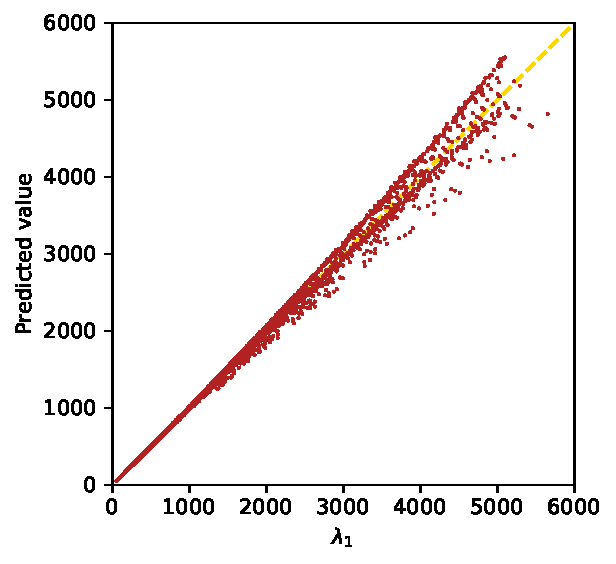
\includegraphics[width = 52mm]{figures/polynomial_4_prediction.pdf}
        \caption{Predviđanja \ensuremath{P_{\numprint{4}}}}
        \label{fig:polynomial_4_prediction}
    \end{subfigure}
    \begin{subfigure}{57mm}
        \centering
        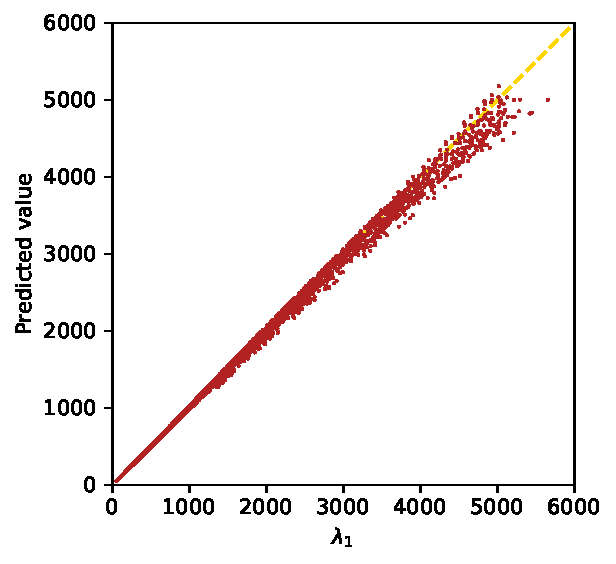
\includegraphics[width = 52mm]{figures/polynomial_5_prediction.pdf}
        \caption{Predviđanja \ensuremath{P_{\numprint{5}}}}
        \label{fig:polynomial_5_prediction}
    \end{subfigure}
    \caption[Predviđanja polinoma]{Predviđanja polinoma. Polinom stupnja $ \numprint{4} $ označen je s $ P_{\numprint{4}} $ i polinom stupnja $ \numprint{5} $ s $ P_{\numprint{5}} $.}
    \label{fig:polynomial_predictions}
\end{figure}

\par

\begin{figure}[htb!]
    \centering
    \begin{subfigure}{57mm}
        \centering
        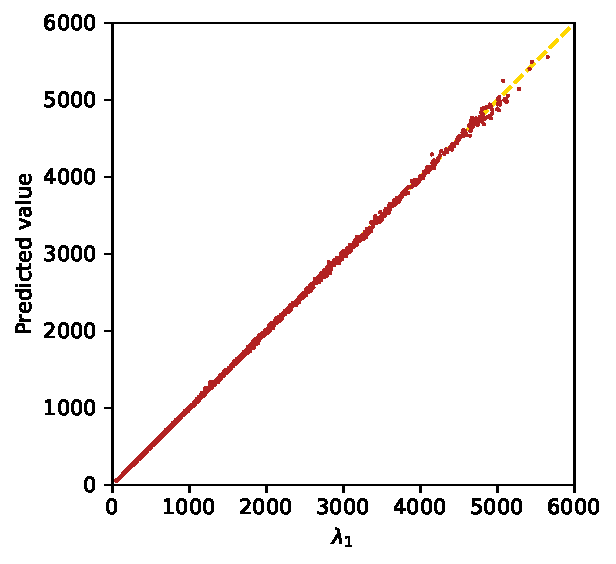
\includegraphics[width = 52mm]{figures/neural_network_prediction.pdf}
        \caption{Predviđanja \emph{NN}}
        \label{fig:neural_network_prediction}
    \end{subfigure}
    \begin{subfigure}{57mm}
        \centering
        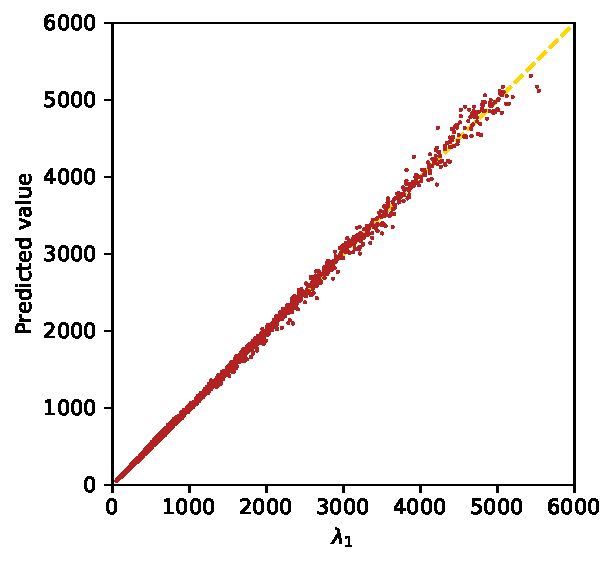
\includegraphics[width = 52mm]{figures/convolutional_neural_network_prediction.pdf}
        \caption{Predviđanja \emph{CNN}}
        \label{fig:convolutional_neural_network_prediction}
    \end{subfigure}
    \caption[Predviđanja neuronske mreže i konvolucijske neuronske mreže]{Predviđanja neuronske mreže i konvolucijske neuronske mreže. Neuronska mreža označena je s \emph{NN} i konvolucijska neuronska mreža s \emph{CNN}.}
    \label{fig:networks_predictions}
\end{figure}

\par%
\clearpage%
\newpage

\begin{figure}[htb!]
    \centering
    \begin{subfigure}{55.5mm}
        \centering
        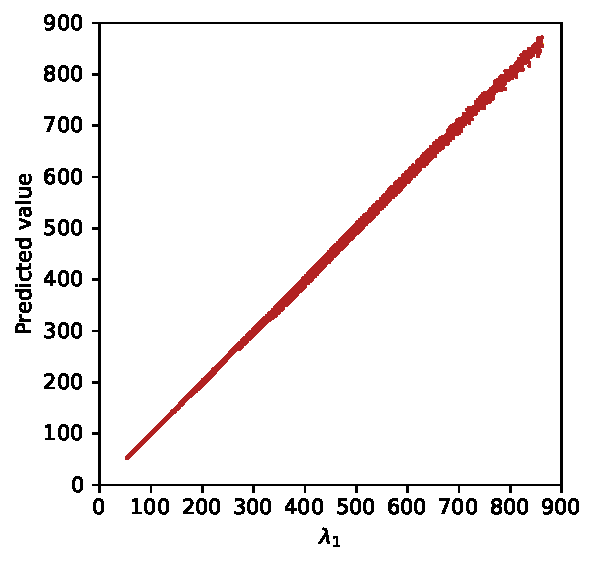
\includegraphics[width = 50.5mm]{figures/polynomial_4_prediction_90_percent.pdf}
        \caption{Predviđanja \ensuremath{P_{\numprint{4}}}}
        \label{fig:polynomial_4_prediction_90_percent}
    \end{subfigure}
    \begin{subfigure}{55.5mm}
        \centering
        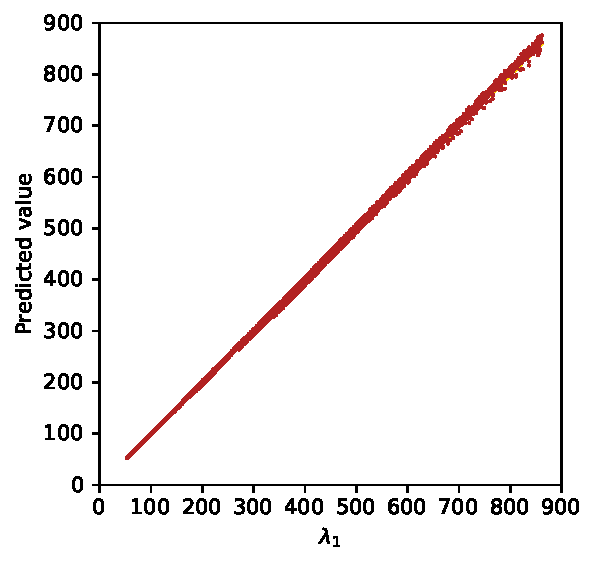
\includegraphics[width = 50.5mm]{figures/polynomial_5_prediction_90_percent.pdf}
        \caption{Predviđanja \ensuremath{P_{\numprint{5}}}}
        \label{fig:polynomial_5_prediction_90_percent}
    \end{subfigure}
    \caption[Predviđanja polinoma na donjih \ensuremath{\unit[\numprint{90}]{\%}} vrijednosti]{Predviđanja polinoma na donjih \ensuremath{\unit[\numprint{90}]{\%}} vrijednosti. Polinom stupnja $ \numprint{4} $ označen je s $ P_{\numprint{4}} $ i polinom stupnja $ \numprint{5} $ s $ P_{\numprint{5}} $.}
    \label{fig:polynomial_predictions_90_percent}
\end{figure}

\par

\begin{figure}[htb!]
    \centering
    \begin{subfigure}{55.5mm}
        \centering
        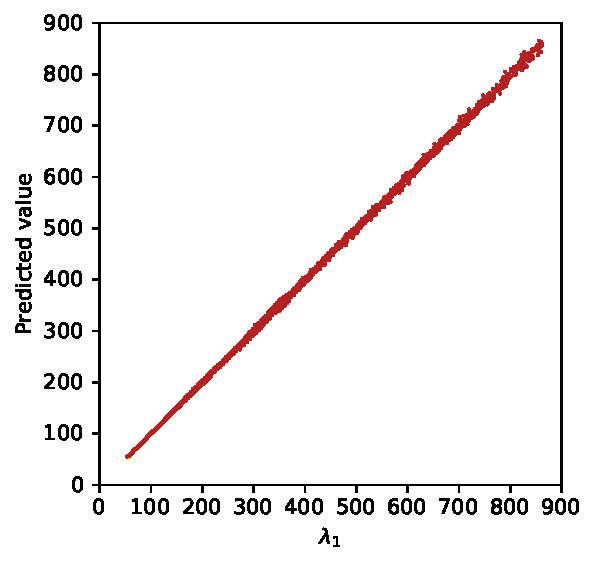
\includegraphics[width = 50.5mm]{figures/neural_network_prediction_90_percent.pdf}
        \caption{Predviđanja \emph{NN}}
        \label{fig:neural_network_prediction_90_percent}
    \end{subfigure}
    \begin{subfigure}{55.5mm}
        \centering
        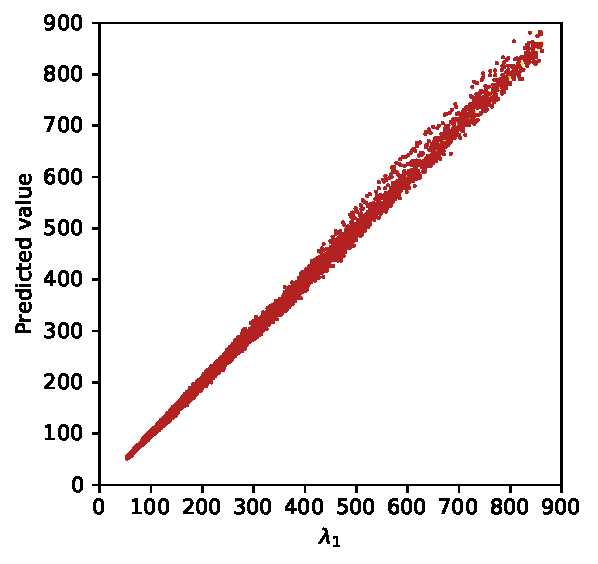
\includegraphics[width = 50.5mm]{figures/convolutional_neural_network_prediction_90_percent.pdf}
        \caption{Predviđanja \emph{CNN}}
        \label{fig:convolutional_neural_network_prediction_90_percent}
    \end{subfigure}
    \caption[Predviđanja neuronske mreže i konvolucijske neuronske mreže na donjih \ensuremath{\unit[\numprint{90}]{\%}} vrijednosti]{Predviđanja neuronske mreže i konvolucijske neuronske mreže na donjih \ensuremath{\unit[\numprint{90}]{\%}} vrijednosti. Neuronska mreža označena je s \emph{NN} i konvolucijska neuronska mreža s \emph{CNN}.}
    \label{fig:networks_predictions_90_percent}
\end{figure}

\par%
\clearpage%
\newpage

\section{Brzine modela}
\label{sec:models_time_consumption}

Za usporedbu brzina modela, modeli su provedeni na kompletnom skupu podataka od $ \numprint{1129741} $ trokuta iako su među njima i trokuti iz testnih i validacijskih skupova. Međutim, za računanje brzine modela točnosti tih predviđanja nisu se proučavale, a skup od više od $ \numprint{1000000} $ trokuta predstavljao je dovoljno velik skup za objektivno mjerenje vremena (više pokretanja iste metode vremenski je vrlo malo variralo). Metode su pokretane na osobnom prijenosnom računalu autora kao jedini korisnikovi pokrenuti procesi nakon pokretanja operacijskog sustava, a svaka metoda pokrenuta je $ \numprint{3} $ puta i kao konačno vrijeme uzeta je aritmetička sredina triju izmjerenih vremena.

\par

Referentno računalo opremljeno je procesorom \emph{\href{https://www.intel.co.uk/}{Intel{\textregistered}} Core{\texttrademark} i$ \numprint{5} $-$ \numprint{7200} $U $ \SI{2.5}{\giga \hertz} $} s \emph{Turbo Boost} ubrzanjem do $ \SI{3.1}{\giga \hertz} $, s $ \SI{8}{\giga \byte} $ \emph{DDR$ \numprint{4} $} radne memorije i s grafičkom karticom \emph{\href{https://www.nvidia.com/}{NVIDIA{\textregistered}} GeForce{\textregistered} GTX $ \numprint{950} $M} s $ \SI{2}{\giga \byte} $ \emph{VRAM}-a. Korišteni operacijski sustav je \href{https://www.linux.org/}{\emph{Linux}} distribucija \emph{\href{https://lubuntu.net/}{Lubuntu} $ \numprint{18} $.$ \numprint{04} $}, prevoditelj programskog jezika \href{https://en.cppreference.com/w/c/header}{\emph{C}} je \emph{\href{https://gcc.gnu.org/}{GCC} $ \numprint{7} $.$ \numprint{4} $.$ \numprint{0} $} i inačica programskog jezika \href{https://docs.python.org/3/}{\emph{Python}} je $ \numprint{3} $.$ \numprint{6} $.$ \numprint{9} $. Inačica paketa \href{https://numpy.org/}{\emph{NumPy}} je $ \numprint{1} $.$ \numprint{17} $.$ \numprint{4} $, paketa \href{https://pandas.pydata.org/}{\emph{Pandas}} $ \numprint{0} $.$ \numprint{25} $.$ \numprint{3} $, paketa \href{https://scikit-learn.org/stable/}{\emph{Scikit-learn}} $ \numprint{0} $.$ \numprint{22} $, paketa \href{https://www.tensorflow.org/}{\emph{TensorFlow}} $ \numprint{1} $.$ \numprint{14} $.$ \numprint{0} $ i paketa \href{https://keras.io/}{\emph{Keras}} $ \numprint{2} $.$ \numprint{3} $.$ \numprint{1} $. Inačica platforme \href{https://developer.nvidia.com/cuda-zone}{\emph{CUDA}} je $ \numprint{10} $.$ \numprint{2} $.$ \numprint{89} $. Interpreter programskog jezika \href{https://freefem.org/}{\emph{FreeFem++}} inačice je $ \numprint{4} $.$ \numprint{400003} $.

\par

Rezultati mjerenja vremena prikazani su u tablici~\ref{tab:computation_times}. Brzina modela konvolucijske neuronske mreže nije izračunata zbog nedostatka resursa, ali i zbog nedovoljno optimiziranog algoritma generiranja vizualizacija trokuta. Naime, na platformi \href{https://colab.research.google.com/}{\emph{Google Colab}} generiranje vizualizacija trokuta, koje bi se smatralo pretprocesiranjem za model konvolucijske neuronske mreže (osnovnim ulaznim podatcima svih modela smatraju se koordinate vrhova trokuta), na $ \numprint{100000} $ trokuta trajalo je dulje od, na primjer, računanja svojstvenih vrijednosti metodom konačnih elemenata na referentnom računalu, koje je slabijih specifikacija.

\par%
\clearpage%
\newpage

\begin{table}[htb!]
    \centering
    \caption[Usporedba vremena metoda računanja]{Usporedba vremena metoda računanja. \emph{FEM} je numerički račun metodom konačnih elemenata, \emph{deskripcija} je računanje duljina stranica i veličina vanjskih kutova, \emph{uređenje} je poredanje duljina stranica u padajući poredak i veličina vanjskih kutova u rastući, \emph{karakterizacija} je računanje koordinata karakteristične točke (\seetxt~propoziciju~\ref{prop:triangle_characteristic_bijective}) iz rezultata \emph{deskripcije}, a \emph{SVD} je računanje singularnih vrijednosti duljina stranica i vanjskih kutova iz rezultata \emph{deskripcije}.}
    \label{tab:computation_times}
    \begin{tabular}{| c | l | r  r |}
        \hline
        \multicolumn{1}{| c |}{Područje} & \multicolumn{1}{c |}{Opis} & \multicolumn{1}{c}{Apsolutno vrijeme} & \multicolumn{1}{c |}{Relativno vrijeme} \\
        \hline
        \multirow{1}{*}{Numerički račun} & \emph{FEM} & $ \SI{948.754328}{\second} $ & $ \numprint{1.000000} $ \\
        \hline
        \multirow{4}{*}{Pretprocesiranje} & Deskripcija & $ \SI{0.180276}{\second} $ & $ \numprint{0.000190} $ \\
         & Uređenje & $ \SI{0.080183}{\second} $ & $ \numprint{0.000085} $ \\
         & Karakterizacija & $ \SI{0.054539}{\second} $ & $ \numprint{0.000057} $ \\
         & \emph{SVD} & $ \SI{4.821884}{\second} $ & $ \numprint{0.005082} $ \\
        \hline
        \multirow{3}{*}{Predviđanje} & Polinom stupnja $ \numprint{4} $ & $ \SI{0.433055}{\second} $ & $ \numprint{0.000456} $ \\
         & Polinom stupnja $ \numprint{5} $ & $ \SI{0.690426}{\second} $ & $ \numprint{0.000728} $ \\
         & Neuronska mreža & $ \SI{1.014543}{\second} $ & $ \numprint{0.001069} $ \\
        \hline
    \end{tabular}
\end{table}

\par

Iz tablice~\ref{tab:computation_times} možemo zaključiti da je, i ako ubrojimo odgovarajuće pretprocesiranje, polinom stupnja $ \numprint{4} $ od klasičnog numeričkog računa brži čak više od $ \numprint{1422} $ puta, a polinom stupnja $ \numprint{5} $ brži je više od $ \numprint{1025} $ puta. Neuronska mreža brža je više od $ \numprint{155} $ puta, pri čemu skoro $ \unit[80]{\%} $ vremena za model neuronske mreže zauzima \emph{SVD}. Ako se \emph{SVD} trokuta može vremenski optimizirati, takvo bi poboljšanje moglo bitno ubrzati ovaj model.

\par

\section{Minimizacija najmanje svojstvene vrijednosti Laplaceovog operatora}
\label{sec:minimal_Laplace_eigenvalue_minimisation}

Osim po globalnoj uspješnosti i brzini, modeli su testirani i u simuliranom primjeru stvarne primjene. U tu je svrhu uzet problem minimizacije najmanje svojstvene vrijednosti na trokutima fiksnog opsega. Najmanja svojstvena vrijednost Laplaceovog operatora morala bi se postizati na jednakostraničnom trokutu, što proizlazi iz nejednakosti vezanih uz površinu skupa koje je Siudeja naveo u~\cite{bib:Siudeja08} i Heronove formule za površinu trokuta. Laugesen i Siudeja u~\cite{bib:Laugesen10} također su iskazali da, osim među trokutima fiksnog opsega ili fiksne površine, jednakostranični trokut najmanju svojstvenu vrijednost minimizira i među trokutima fiksnog dijametra, što se može i naslutiti iz slike~\ref{fig:triangles_eigenvalues}.

\par

Proučavana su dva problema minimizacije. Jedan je u $ \numprint{6} $-dimenzionalnom prostoru, to jest, pronalazak (nekih) vrijednosti $ x_{\numprint{1}} , y_{\numprint{1}} , x_{\numprint{2}} , y_{\numprint{2}} , x_{\numprint{3}} , y_{\numprint{3}} \in \reals $ takvih da je trokut čiji su vrhovi dani koordinatama $ \left( x_{\numprint{1}} , y_{\numprint{1}} \right) , \left( x_{\numprint{2}} , y_{\numprint{2}} \right) , \left( x_{\numprint{3}} , y_{\numprint{3}} \right) \in \reals^{\numprint{2}} $ u standardnoj bazi opsega $ \numprint{3} $ i da među takvim trokutima on postiže najnižu najmanju svojstvenu vrijednost Laplaceovog operatora---teorem~\ref{thm:Laplacian_eigenvalue_similar_domains} odnosno korolar~\ref{cor:spectrum_similar_domains} pokazuju da takvih (jednakostraničnih) trokuta ima neprebrojivo beskonačno mnogo, ali su svi oni jednaki do na izometrične transformacije. Drugi je problem u $ \numprint{1} $-dimenzionalnom prostoru, to jest, pronaći vrijednost $ \varphi \in \intervaloo{\numprint{0}}{\pi} $ takvu da trokut čiji su vrhovi dani koordinatama $ \left( \frac{\numprint{1}}{\numprint{2}} , \numprint{0} \right) , \left( \cos \varphi , \frac{\sqrt{\numprint{3}}}{\numprint{2}} \sin \varphi \right) , \left( {- \frac{\numprint{1}}{\numprint{2}}} , \numprint{0} \right) \in \reals^{\numprint{2}} $ u standardnoj bazi među takvim trokutima postiže najnižu najmanju svojstvenu vrijednost---ovdje je rješenje jedinstveno i iznosi $ \varphi = \frac{\pi}{\numprint{2}} $ (uz uvjet $ \varphi \in \intervaloo{{- \pi}}{\pi} \setminus \left\{ \numprint{0} \right\} $ rješenja bi bila $ \varphi = {\pm \frac{\pi}{\numprint{2}}} $, a za $ \varphi \in \reals \setminus \left\{ k \pi \in \reals : k \in \integers \right\} $ sva su rješenja od ovih udaljena za višekratnike broja $ \numprint{2} \pi $). U oba slučaja optimalni trokut bio bi onakav trokut čije su sve stranice duljine $ \numprint{1} $, stoga su u daljnjem tekstu navedene apsolutne greške ujedno i relativne greške.

\par

Minimizacije su vršene funkcijom \href{https://docs.scipy.org/doc/scipy/reference/generated/scipy.optimize.minimize.html}{\lstinline[language = Python, style = program]{scipy.optimize.minimize}} s odgovarajućim ograničenjima: stranice ne smiju biti duljine $ \numprint{0} $, vanjski kutovi moraju biti u intervalu $ \intervaloo{\numprint{0}}{\pi} $, opseg mora biti jednak $ \numprint{3} $, parametar $ \varphi $ mora biti u intervalu $ \intervaloo{\numprint{0}}{\pi} $. Inicijalni pokušaji generirani su pseudoslučajno.

\par

Polinom stupnja $ \numprint{4} $ u oba problema minimizacije uvijek je konvergirao k jednakostraničnom trokutu. Greške su kod tog polinoma po duljinama stranica bile reda $ \numprint{10}^{{- \numprint{3}}} $ u prvom problemu odnosno $ \numprint{10}^{{- \numprint{9}}} $ u drugom problemu. Polinom stupnja $ \numprint{5} $ također je konvergirao k jednakostraničnom trokutu, a njegove su greške po duljinama stranica bile reda $ \numprint{10}^{{- 4}} $ u prvom problemu odnosno $ \numprint{10}^{{- \numprint{9}}} $ u drugom problemu. Neuronska mreža i konvolucijska neuronska mreža u oba problema ponekad konvergiraju k jednakostraničnom trokutu s točnostima reda $ \numprint{10}^{{- \numprint{2}}} $ ili boljim, međutim, ponekad (možda čak i češće) ne konvergiraju k takvom trokutu. Uzajamne pravilnosti kod neuronske mreže i konvolucijske neuronske mreže nisu uočene: ponekad nijedna ne konvergira, ponekad samo jedna od njih konvergira, a ponekad obje konvergiraju i to čak i ako inicijalni pokušaj nije \emph{blizu} rješenja. Jedan proces minimizacije u $ \numprint{1} $-dimenzionalnom prostoru prikazan je na slikama od~\ref{fig:polynomial_4_minimisation} do~\ref{fig:convolutional_neural_network_minimisation}.

\par%
\clearpage%
\newpage

\begin{figure}[htb!]
    \centering
    \begin{subfigure}{53mm}
        \centering
        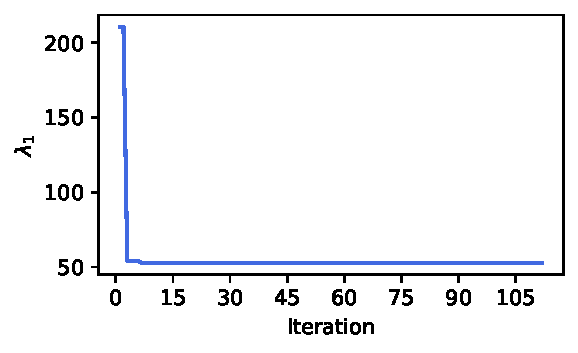
\includegraphics[width = 48mm]{figures/polynomial_4_minimisation_values.pdf}
        \caption{Konvergencija predviđene vrijednosti}
        \label{fig:polynomial_4_minimisation_values}
    \end{subfigure}
    \begin{subfigure}{52mm}
        \centering
        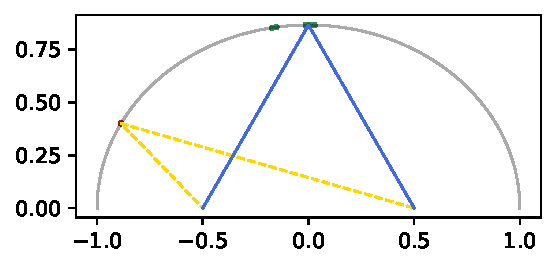
\includegraphics[width = 47mm]{figures/polynomial_4_minimisation_vertices.pdf}
        \caption{Konvergencija vrha}
        \label{fig:polynomial_4_minimisation_vertices}
    \end{subfigure}
    \caption[Minimizacija najmanje svojstvene vrijednosti Laplaceovog operatora polinomom stupnja \ensuremath{\numprint{4}}]{Minimizacija najmanje svojstvene vrijednosti Laplaceovog operatora polinomom stupnja \ensuremath{\numprint{4}}. Na slici~\ref{fig:polynomial_4_minimisation_vertices} vrhovi su obojani s obzirom na predviđenu vrijednost: u crvenim vrhovima je predviđena viša, a u zelinima niža vrijednost. Inicijalni trokut označen je iscrtkanom žutom linijom dok je rezultantni trokut označen punom plavom linijom.}
    \label{fig:polynomial_4_minimisation}
\end{figure}

\par

\begin{figure}[htb!]
    \centering
    \begin{subfigure}{53mm}
        \centering
        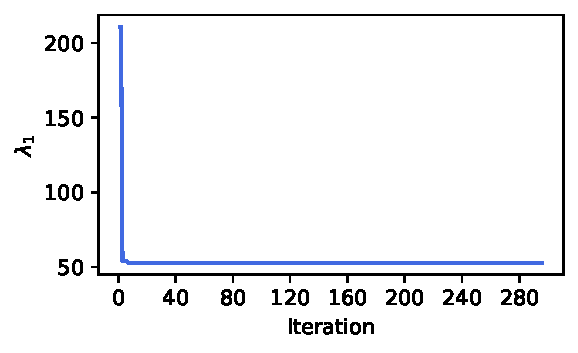
\includegraphics[width = 48mm]{figures/polynomial_5_minimisation_values.pdf}
        \caption{Konvergencija predviđene vrijednosti}
        \label{fig:polynomial_5_minimisation_values}
    \end{subfigure}
    \begin{subfigure}{52mm}
        \centering
        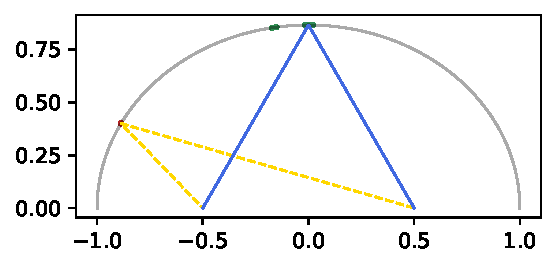
\includegraphics[width = 47mm]{figures/polynomial_5_minimisation_vertices.pdf}
        \caption{Konvergencija vrha}
        \label{fig:polynomial_5_minimisation_vertices}
    \end{subfigure}
    \caption[Minimizacija najmanje svojstvene vrijednosti Laplaceovog operatora polinomom stupnja \ensuremath{\numprint{5}}]{Minimizacija najmanje svojstvene vrijednosti Laplaceovog operatora polinomom stupnja \ensuremath{\numprint{5}}. Na slici~\ref{fig:polynomial_5_minimisation_vertices} vrhovi su obojani s obzirom na predviđenu vrijednost: u crvenim vrhovima je predviđena viša, a u zelinima niža vrijednost. Inicijalni trokut označen je iscrtkanom žutom linijom dok je rezultantni trokut označen punom plavom linijom.}
    \label{fig:polynomial_5_minimisation}
\end{figure}

\par%
\clearpage%
\newpage

\begin{figure}[htb!]
    \centering
    \begin{subfigure}{53mm}
        \centering
        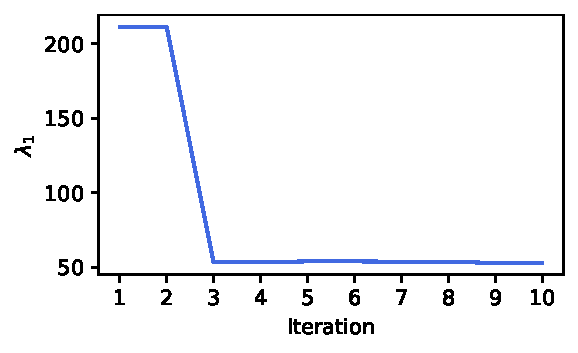
\includegraphics[width = 48mm]{figures/neural_network_minimisation_values.pdf}
        \caption{Konvergencija predviđene vrijednosti}
        \label{fig:neural_network_minimisation_values}
    \end{subfigure}
    \begin{subfigure}{52mm}
        \centering
        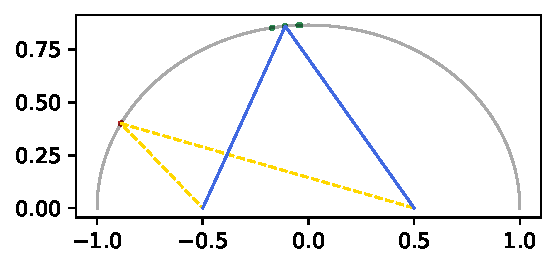
\includegraphics[width = 47mm]{figures/neural_network_minimisation_vertices.pdf}
        \caption{Konvergencija vrha}
        \label{fig:neural_network_minimisation_vertices}
    \end{subfigure}
    \caption[Minimizacija najmanje svojstvene vrijednosti Laplaceovog operatora neuronskom mrežom]{Minimizacija najmanje svojstvene vrijednosti Laplaceovog operatora neuronskom mrežom. Na slici~\ref{fig:neural_network_minimisation_vertices} vrhovi su obojani s obzirom na predviđenu vrijednost: u crvenim vrhovima je predviđena viša, a u zelinima niža vrijednost. Inicijalni trokut označen je iscrtkanom žutom linijom dok je rezultantni trokut označen punom plavom linijom.}
    \label{fig:neural_network_minimisation}
\end{figure}

\par

\begin{figure}[htb!]
    \centering
    \begin{subfigure}{53mm}
        \centering
        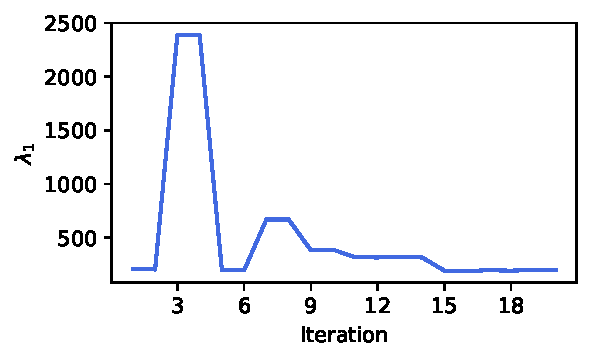
\includegraphics[width = 48mm]{figures/convolutional_neural_network_minimisation_values.pdf}
        \caption{Konvergencija predviđene vrijednosti}
        \label{fig:convolutional_neural_network_minimisation_values}
    \end{subfigure}
    \begin{subfigure}{52mm}
        \centering
        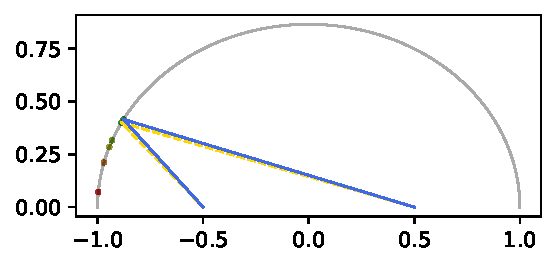
\includegraphics[width = 47mm]{figures/convolutional_neural_network_minimisation_vertices.pdf}
        \caption{Konvergencija vrha}
        \label{fig:convolutional_neural_network_minimisation_vertices}
    \end{subfigure}
    \caption[Minimizacija najmanje svojstvene vrijednosti Laplaceovog operatora konvolucijskom neuronskom mrežom]{Minimizacija najmanje svojstvene vrijednosti Laplaceovog operatora konvolucijskom neuronskom mrežom. Na slici~\ref{fig:convolutional_neural_network_minimisation_vertices} vrhovi su obojani s obzirom na predviđenu vrijednost: u crvenim vrhovima je predviđena viša, a u zelinima niža vrijednost. Inicijalni trokut označen je iscrtkanom žutom linijom dok je rezultantni trokut označen punom plavom linijom.}
    \label{fig:convolutional_neural_network_minimisation}
\end{figure}

\par

Pojava da polinomni modeli uspijevaju minimizirati najmanju svojstvenu vrijednost Laplaceovog operatora mogla se pretpostaviti s obzirom na to da su vrlo uspješni u predviđanju niskih vrijednosti (\seetxt~tablice~\ref{tab:models_rmse} i \ref{tab:models_mape}). Autor ovog rada, doduše, nije uspio objasniti zašto modeli neuronske mreže i konvolucijske neuronske mreže nisu pouzdani modeli u proučavanim problemima minimizacije. Štoviše, ostalo je neobjašnjeno zašto se minimizacija tim modelima izvršava u osjetno manjem broju iteracija, pri čemu neuronska mreža nerijetko izvrši svega $ \numprint{4} $ -- $ \numprint{6} $ iteracija nakon čega se postiže \emph{prividna konvergencija} i minimizacija završava.

\par


    % Zakljucak.
    \addchap{Zaključak}

Od razvijenih modela, za male vrijednosti najmanje svojstvene vrijednosti Laplaceovog operatora (ispod $ \numprint{200} $) najbolju alternativu klasičnom numeričkom računu predstavljaju polinomni modeli kao najbrži i najtočniji. Štoviše, za vrijednosti ispod $ \numprint{100} $ njihova točnost je $ {\pm \numprint{0.1}} $. Međutim, na višim vrijednostima njihova uspješnost znantno opada i postaju vrlo nepouzdani predviditelji. S druge strane, model neuronske mreže najtočniji je na većim vrijednostima, iako i njegova točnost na većim vrijednostima također počinje opadati. Model konvolucijske neuronske mreže među svim je modelima najlošiji na manjim vrijednostima, ali njegova točnost relativno sporije opada s porastom ciljne varijable.

\par

Razlog zašto su svi modeli znatno lošiji na većim vrijednostima mogao bi biti rijetkost zastupljenosti primjera u tim kvantilima---najviših $ \unit[\numprint{5}]{\%} $ vrijednosti u intervalu je širine više od $ \numprint{4000} $, a preostalih $ \unit[\numprint{95}]{\%} $ u intervalu je širine manje od $ \numprint{2000} $. Osim manjkavosti metodologije, moguće je i da je ciljna varijabla u tom području \emph{jako} različita za trokute koji se \emph{malo} razlikuju---ovo, uostalom, sugerira slika~\ref{fig:triangles_eigenvalues}---čime je njezinu vrijednost teže predvidjeti ako je ona jako visoka. Ipak, prije kritiziranja modela zbog nepouzdanosti na tako velikom intervalu treba uzeti u obzir sliku~\ref{fig:triangles_eigenvalues}, na kojoj se vidi da trokutima na kojima najmanja svojstvena vrijednost upada u gornjih $ \unit[\numprint{10}]{\%} $ proučavanih vrijednosti (donja granica tog kvantila iznosi otprilike $ \numprint{861.51} $, dok je minimum oko $ \numprint{52.72} $ i maksimum oko $ \numprint{5938.19} $)---\emph{najžutije}/\emph{najnarančastije} dvije zone na slici~\ref{fig:triangles_eigenvalues_contour}---vrijednost ordinate karakteristične točke iz propozicije~\ref{prop:triangle_characteristic_bijective} ne postiže ni $ \numprint{0.15} $. Preostalih $ \unit[\numprint{90}]{\%} $ trokuta, na kojima su modeli znatno uspješniji, zauzima puno veći dio skupa $ D_{{\bigtriangleup}} $ iz propozicije~\ref{prop:triangle_characteristic_bijective}.

\par

Valja uočiti da su tri kategorije modela, osim što se kategorički razlikuju, razvijene iz tri različita aspekta: linearne regresije u obzir uzimaju samo koordinate karakteristične točke iz propozicije~\ref{prop:triangle_characteristic_bijective}, neuronska mreža u obzir uzima duljine stranica, veličine vanjskih kutova i singularne vrijednosti duljina stranica i vanjskih kutova, a konvolucijska neuronska mreža u obzir uzima samo vizualizaciju trokuta. Kombinacije modela, to jest, pristupa predviđanju također predstavljaju moguće poboljšanje njihove uspješnosti. Rezultati razvijenih modela, kao i eksploratorna analiza numeričkih podataka, sugeriraju da bi takve kombinacije mogle biti uspješne.

\par%
\clearpage%
\newpage

Nastavak istraživanja predstavlja i generalizacija modela na ostale poligone. Najveći potencijal u tome ima konvolucijska neuronska mreža, a najmanji polinomna rješenja. Naime, kompleksnost konvolucijske neuronske mreže ne ovisi o broju kutova odnosno stranica tako da je na slici iste veličine moguće prikazati bilo koji oblik (i to ne nužno samo poligonalni). Doduše, pregruba rezolucija prikaza mogla bi \emph{skrivati} neke eventualno ključne informacije, ali funkcija dubine iz definicije~\ref{def:set_deepness} donekle osigurava da se oblik vizualiziranog skupa može rekonstruirati i u slučaju pregrube rezolucije. S druge strane, broj članova polinoma stupnja $ d \in \naturals $ u $ \numprint{2} k $ varijabli (koliko bi bilo koordinata karakteristične točke $ \left( k + \numprint{2} \right) $-gona), za $ k \in \naturals $, $ k \geq \numprint{3} $, iznosi $ \binom{\numprint{2} k + d}{d} $, što znači da kompleksnost polinomnih rješenja raste brzinom reda $ \bigO \left( n^{d} \right) $ s porastom broja vrhova. Iako je neuronska mreža možda \emph{prekompleksna} s obzirom na veličinu ulaza i korištene aktivacijske funkcije, jednostavnije arhitekture lučile su bitno lošije rezultate, a ovakva neuronska mreža možda bi, samo uz podešavanje veličine ulaza ili još uz eventualno malu izmjenu skrivenih slojeva, mogla predstavljati dobar model i za druge poligone. Ipak, sam ulaz s porastom broja kutova raste brzinom reda $ \bigO \left( n \right) $, stoga ni takav model nije dobar kandidat za poligone s velikim brojem vrhova.

\par

Osim rasta kompleksnosti modela, polinomni modeli i neuronska mreža ograničeni su i time da mogu predviđati nužno na jednoj klasi poligona---svi poligoni moraju imati isti broj vrhova. Da bismo konstruirali model koji bi mogao predviđati ciljnu varijablu na svim $ k $-gonima za $ k \leq m $, gdje je $ m \in \naturals $, $ m \geq \numprint{3} $, unaprijed zadan, za te modele bilo bi potrebno definirati konvenciju kojom se, na primjer, trokut prikazuje kao peterokut---to bi moglo biti tako da najdulju stranicu \emph{raspolovimo} (kao novi vrh postavljamo njezino polovište) i tako činimo dok broj vrhova nije zadovoljen---ili bi se broj primjera kod treniranja morao znatno povećati tako da se u obzir uzme što više mogućih izbora nepravih vrhova. Potonja opcija povećava kompleksnost treniranja, ali se zbog neprekidnosti spektra (\seetxt~teorem~\ref{thm:Laplace_eigenvalue_continuity}) čini boljom opcijom jer, na primjer, niz pravih osmerokuta može konvergirati k pravom sedmerokutu čak i ako nijedan vrh osmerokuta ne konvergira k polovištu neke stranice sedmerokuta.

\par

Konvolucijska neuronska mreže možda bi mogla biti uspješnija kada bi bili dostupni veći resursi, čime bi se mogla i \emph{vratiti} izostavljena $ \numprint{3} $ sloja ($ \numprint{1} $ redukcijski i $ \numprint{2} $ neredukcijska) i čime bi se mreža mogla dulje trenirati. S obzirom na mali broj epoha, a s druge strane kompleksnost ulaza i veličinu njezine arhitekture, postignuti rezultati iznenađujuće su dobri. Ionako je takva konvolucijska neuronska mreža na drugom problemu vezanom uz diferencijalne jednadžbe postizala odlične rezultate, kako su objasnili Mills i dr.\ u~\cite{bib:Mills17}, gdje su je predstavili, tako da bi valjalo daljnje istraživanje usmjeriti i prema njezinom poboljšanju.

\par%
\clearpage%
\newpage

Poboljšanja modela konvolucijske neuronske mreže mogu biti i izmjene vizualizacije---možda je izbor vizualizacije trokuta funkcijom dubine neadekvatan za ovaj problem, što bi moglo negativno utjecati na uspješnost ovog modela. Na primjer, problem bi kod odabrane vizualizacije mogao biti što rub poligona (trokuta) nije jasno vidljiv, nego vrijednosti postepeno padaju u $ \numprint{0} $ (\seetxt~sliku~\ref{fig:triangle_deepness}). Ovo bi se moglo riješiti polovičnim normiranjem funkcije dubine tako da na jednakostraničnom trokutu ona poprima $ \frac{\numprint{1}}{\numprint{2}} $ i da se takva vizualizacijska matrica tada zbroji s $ \frac{\numprint{1}}{\numprint{2}} $ vizualizacijske matrice sa slike~\ref{fig:triangle_mesh}.

\par

Međutim, s obzirom na brzine polinomnih modela i neuronske mreže, ali i njihovih točnosti barem na nekim trokutima, isplativo bi bilo baviti se i njihovim daljnjim razvoje. Na poligonima s manjim brojem vrhova, ako je ove modele moguće generalizirati i eventualno poboljšati, takvi modeli predstavljaju brzu alternativu klasičnom numeričkom računu, a pogotovo egzaktnom računu. Možda je i računanje najmanje svojstvene vrijednosti Laplaceovog operatora metodom konačnih elemenata na promatranim trokutima usporeno načinom na koji je taj program napisan i/ili kvalitetama odabranog programskog jezika \href{https://freefem.org/}{\emph{FreeFem++}}, ali tablica~\ref{tab:computation_times} sugerira da se konkurentno brzi rezultati tom metodom vjerojatno ne mogu postići.

\par

Osim teme ovog rada, s obzirom na dobivene rezultate na ovom području potencijalnim nastavkom istraživanja čine se i definirane singularne vrijednosti duljina stranica i vanjskih kutova poligona. Autor ovog rada tako definirane ni tako nazvane vrijednosti nije pronašao u literaturi, ali kroz eksploratornu analizu i dobivene rezultate, barem na trokutima, čini se da su one vrlo informativne o obliku poligona. Naime, u poglavlju~\ref{chp:Dirichlet_Laplacian} već je navedeno kako su Reuter i dr.\ objasnili u~\cite{bib:Reuter09} da je u praksi dovoljno poznavati najmanjih konačno mnogo vrijednosti spektra skupa da bi se moglo zaključivati o njegovu obliku, stoga je najmanja svojstvena vrijednost Laplaceovog operatora uvjetovana oblikom poligona. S druge strane, slika~\ref{fig:singular_value_eigenvalue}, izračunati koeficijenti korelacije i rezultati modela neuronske mreže sugeriraju da su i definirane singularne vrijednosti relativno ovisne o toj vrijednosti odnosno da postoji ovisnost u obratnom smjeru.

\par


    %%  KRAJNJI DIO

    % Bibliografija.
%   \nocite{*}%
    \printbibliography[heading = master]%
%   \printbibliography[title = {Primjer bibliografije}, heading = master, keyword = example]

    \backmatter

    % Sazetak na hrvatskom jeziku.
    \begin{sazetak}
    Proučavajući teorijski svojstvene vrijednosti i svojstvene funkcije Laplaceovog operatora uočena su obilježja kojima se njihovo računanje može pojednostaviti. Prvenstveno, one ne ovise o afinim izometričnim transformacijama skupova (osim što se domena svojstvenih funkcija, očito, izometrično transformira). Također, skaliranjem skupa svojstvene se vrijednosti skaliraju multiplikativnim inverzom kvadrata skalara, dok se svojstvene funkcije komponiraju zdesna sa skalarom. Nadalje, one neprekidno ovise o domeni i svojstvene su vrijednosti padajuće s obzirom na relaciju inkluzije. Iz svega se navedenog zaključeno je da se određene domene u svrhu numeričkog računanja svojstvenih vrijednosti i svojstvenih funkcija Laplaceovog operatora (to jest, najmanje svojstvene vrijednosti u slučaju ovog rada) mogu aproksimirati \emph{jednostavnijim}, \emph{dovoljno sličnim} i normaliziranim domenama.

    \par

    Kao jedan tip jednostavnijih domena koje mogu poprimiti \emph{razne} oblike odabrani su poligoni. Zbog opaženih obilježja svojstvenih vrijednosti i svojstvenih funkcija Laplaceovog operatora, u svrhu njihova računanja modelom strojnog učenja bilo je poželjno poligone opisati karakterizacijama koje su dovoljno diskriminirajuće, ali i robusne na određene transformacije. U radu su ponuđene nude tri različite karakterizacije poligona, a u praktičnom nastavku rada proučavani su samo trokuti kao prototipi poligona.

    \par

    Za svaku od karakterizacija, nakon proučavanja literature i eksploratorne analize izrađenog skupa podataka, odabrana je jedna pogodna metoda strojnog učenja za početni problem. Tako su konstruirani dva modela linearne regresije, neuronska mreža i konvolucijska neuronska mreža. Nakon treniranja modela njihove su uspješnosti ispitane na testnim skupovima podataka i modeli su uspoređeni s obzirom na uspješnosti i brzine. Rezultati su u većini slučajeva bili obećavajući, ali generalizabilnost modela na složenije poligone nije potvrđena jer model koji se najjednostavnije može generalizirati---konvolucijska neuronska mreža---luči najlošije rezultate.

    \par
\end{sazetak}


    % Sazetak na engleskom jeziku.
    \begin{summary}
    Studying the theory behind the eigenvalues and the eigenfunctions of Dirichlet Laplacian it was observed that they possess some characteristics that allow us to simplify calculations to find them. First of all, they are independent of affine isometric transformations of sets (except that the domain of the eigenfunctions is obviously isometrically transformed). Also, scaling a set scales its eigenvalues by the factor of the square of the multiplicative inverse of the scaling factor, and the resulting eigenfunctions are compositions of the original eigenfunctions on the left and the scaling factor on the right. Furthermore, they depend continuously on the domain and the eigenvalues are monotonically decreasing in regard to the order of inclusion of sets. Considering all this it was then concluded that some domains can be approximated by other, \emph{simpler} yet \emph{similar enough}, normalised domains to numerically find the eigenvalues and the eigenfunctions of Dirichelt Laplacian (i.\ e.\ the minimal eigenvalue, as is the case in this paper) on them.

    \par

    Polygons were then chosen as an example of \emph{simple} domains with \emph{many} different shapes. Because of the observed characteristics of the eigenvalues and the eigenfunctions, to predict them on polygons using a machine learning model, polygons should be characterised in a way that discriminates them but is also resistant to specific transformations. In this paper three distinct characterisations were proposed, and then in the following part of the paper, the practical part, only triangles were observed as they can be considered prototypes of polygons.

    \par

    After studying the sources and conducting exploratory analysis of the generated dataset, a suitable machine learning method was chosen for each of the characterisations to solve the original problem. Subsequently two linear regression models, a neural network, and a convolutional neural network were designed. After the training their success was measured on testing datasets and they were compared for their successfulness and time consumption. In most cases the results were promising, although generalisability of the models to more complex polygons was not confirmed since the model that could be generalised most easily---the convolutional neural network---yeilds the worst results.

    \par
\end{summary}


    % Curriculum vitae.
    \begin{cv}
    Davor Penzar rođen je \DTMdate{1995-11-13} u Zagrebu. Od $ \numprint{2010} $.\ do $ \numprint{2014} $.\ godine pohađao je \href{http://www.gimnazija-klasicna-zg.skole.hr/}{\emph{Klasičnu gimnaziju}} u Zagrebu po nastavljačkom programu učenja latinskog i antičkoga helenskog jezika, a \href{https://www.ncvvo.hr/}{\emph{Državnu maturu}} položio je $ \numprint{2014} $.\ godine. Osim općeobrazovne srednje škole, od $ \numprint{2011} $.\ do $ \numprint{2015} $.\ godine pohađao je i srednju muzičku školu na \emph{Teorijskom odjelu} \href{http://www.ellybasic.hr/}{\emph{Glazbenog učilišta Elly Bašić}} u Zagrebu, koju je maturirao $ \numprint{2015} $.\ godine obranivši završni rad \emph{\emph{Glazbeno učilište Elly Bašić}: $ \numprint{1965} $.\ -- $ \numprint{2015} $.}\ pod voditeljstvom Nataše Perak-Lovričević, prof.

    \par

    Penzar je preddiplomski sveučilišni studij \href{https://www.math.pmf.unizg.hr/hr/preddiplomski-sveu\%C4\%8Dili\%C5\%A1ni-studij-matematika}{\emph{Matematika}} pohađao od $ \numprint{2014} $.\ do $ \numprint{2017} $.\ godine na \href{https://www.math.pmf.unizg.hr/hr}{\emph{Matematičkom odsjeku}} \href{https://www.pmf.unizg.hr/}{\emph{Prirodoslovno-matematičkog fakulteta}} \href{http://www.unizg.hr/}{\emph{Sveučilišta u Zagrebu}}. Na istom je fakultetu $ \numprint{2017} $.\ godine, položivši te godine spomenuti preddiplomski studij i stekavši titulu \emph{sveučilišnog prvostupnika matematike} (\emph{univ.\ bacc.\ math.}), upisao i sveučilišni diplomski studij \href{https://www.math.pmf.unizg.hr/hr/diplomski-sveu\%C4\%8Dili\%C5\%A1ni-studij-ra\%C4\%8Dunarstvo-i-matematika-0}{\emph{Računarstvo i matematika}}.% Na drugoj godini diplomskog studija, godine $ \numprint{2018} $., postao je stipendist \emph{Hrvatske lutrije}.

    \par

    Godine $ \numprint{2017} $.\ Penzar je položio \href{https://www.ets.org/toefl/ibt/about}{\emph{TOEFL iBT}} s ukupno $ \numprint{110} $ bodova od maksimalno mogućih $ \numprint{120} $ bodova. Osim engleskog jezika, tečan je i u komunikaciji na svom materinskom, hrvatskom jeziku.

    \par
\end{cv}

\end{document}
